% Options for packages loaded elsewhere
\PassOptionsToPackage{unicode}{hyperref}
\PassOptionsToPackage{hyphens}{url}
%
\documentclass[
]{article}
\usepackage{amsmath,amssymb}
\usepackage{lmodern}
\usepackage{iftex}
\ifPDFTeX
  \usepackage[T1]{fontenc}
  \usepackage[utf8]{inputenc}
  \usepackage{textcomp} % provide euro and other symbols
\else % if luatex or xetex
  \usepackage{unicode-math}
  \defaultfontfeatures{Scale=MatchLowercase}
  \defaultfontfeatures[\rmfamily]{Ligatures=TeX,Scale=1}
\fi
% Use upquote if available, for straight quotes in verbatim environments
\IfFileExists{upquote.sty}{\usepackage{upquote}}{}
\IfFileExists{microtype.sty}{% use microtype if available
  \usepackage[]{microtype}
  \UseMicrotypeSet[protrusion]{basicmath} % disable protrusion for tt fonts
}{}
\makeatletter
\@ifundefined{KOMAClassName}{% if non-KOMA class
  \IfFileExists{parskip.sty}{%
    \usepackage{parskip}
  }{% else
    \setlength{\parindent}{0pt}
    \setlength{\parskip}{6pt plus 2pt minus 1pt}}
}{% if KOMA class
  \KOMAoptions{parskip=half}}
\makeatother
\usepackage{xcolor}
\usepackage[margin=1in]{geometry}
\usepackage{color}
\usepackage{fancyvrb}
\newcommand{\VerbBar}{|}
\newcommand{\VERB}{\Verb[commandchars=\\\{\}]}
\DefineVerbatimEnvironment{Highlighting}{Verbatim}{commandchars=\\\{\}}
% Add ',fontsize=\small' for more characters per line
\usepackage{framed}
\definecolor{shadecolor}{RGB}{248,248,248}
\newenvironment{Shaded}{\begin{snugshade}}{\end{snugshade}}
\newcommand{\AlertTok}[1]{\textcolor[rgb]{0.94,0.16,0.16}{#1}}
\newcommand{\AnnotationTok}[1]{\textcolor[rgb]{0.56,0.35,0.01}{\textbf{\textit{#1}}}}
\newcommand{\AttributeTok}[1]{\textcolor[rgb]{0.77,0.63,0.00}{#1}}
\newcommand{\BaseNTok}[1]{\textcolor[rgb]{0.00,0.00,0.81}{#1}}
\newcommand{\BuiltInTok}[1]{#1}
\newcommand{\CharTok}[1]{\textcolor[rgb]{0.31,0.60,0.02}{#1}}
\newcommand{\CommentTok}[1]{\textcolor[rgb]{0.56,0.35,0.01}{\textit{#1}}}
\newcommand{\CommentVarTok}[1]{\textcolor[rgb]{0.56,0.35,0.01}{\textbf{\textit{#1}}}}
\newcommand{\ConstantTok}[1]{\textcolor[rgb]{0.00,0.00,0.00}{#1}}
\newcommand{\ControlFlowTok}[1]{\textcolor[rgb]{0.13,0.29,0.53}{\textbf{#1}}}
\newcommand{\DataTypeTok}[1]{\textcolor[rgb]{0.13,0.29,0.53}{#1}}
\newcommand{\DecValTok}[1]{\textcolor[rgb]{0.00,0.00,0.81}{#1}}
\newcommand{\DocumentationTok}[1]{\textcolor[rgb]{0.56,0.35,0.01}{\textbf{\textit{#1}}}}
\newcommand{\ErrorTok}[1]{\textcolor[rgb]{0.64,0.00,0.00}{\textbf{#1}}}
\newcommand{\ExtensionTok}[1]{#1}
\newcommand{\FloatTok}[1]{\textcolor[rgb]{0.00,0.00,0.81}{#1}}
\newcommand{\FunctionTok}[1]{\textcolor[rgb]{0.00,0.00,0.00}{#1}}
\newcommand{\ImportTok}[1]{#1}
\newcommand{\InformationTok}[1]{\textcolor[rgb]{0.56,0.35,0.01}{\textbf{\textit{#1}}}}
\newcommand{\KeywordTok}[1]{\textcolor[rgb]{0.13,0.29,0.53}{\textbf{#1}}}
\newcommand{\NormalTok}[1]{#1}
\newcommand{\OperatorTok}[1]{\textcolor[rgb]{0.81,0.36,0.00}{\textbf{#1}}}
\newcommand{\OtherTok}[1]{\textcolor[rgb]{0.56,0.35,0.01}{#1}}
\newcommand{\PreprocessorTok}[1]{\textcolor[rgb]{0.56,0.35,0.01}{\textit{#1}}}
\newcommand{\RegionMarkerTok}[1]{#1}
\newcommand{\SpecialCharTok}[1]{\textcolor[rgb]{0.00,0.00,0.00}{#1}}
\newcommand{\SpecialStringTok}[1]{\textcolor[rgb]{0.31,0.60,0.02}{#1}}
\newcommand{\StringTok}[1]{\textcolor[rgb]{0.31,0.60,0.02}{#1}}
\newcommand{\VariableTok}[1]{\textcolor[rgb]{0.00,0.00,0.00}{#1}}
\newcommand{\VerbatimStringTok}[1]{\textcolor[rgb]{0.31,0.60,0.02}{#1}}
\newcommand{\WarningTok}[1]{\textcolor[rgb]{0.56,0.35,0.01}{\textbf{\textit{#1}}}}
\usepackage{graphicx}
\makeatletter
\def\maxwidth{\ifdim\Gin@nat@width>\linewidth\linewidth\else\Gin@nat@width\fi}
\def\maxheight{\ifdim\Gin@nat@height>\textheight\textheight\else\Gin@nat@height\fi}
\makeatother
% Scale images if necessary, so that they will not overflow the page
% margins by default, and it is still possible to overwrite the defaults
% using explicit options in \includegraphics[width, height, ...]{}
\setkeys{Gin}{width=\maxwidth,height=\maxheight,keepaspectratio}
% Set default figure placement to htbp
\makeatletter
\def\fps@figure{htbp}
\makeatother
\setlength{\emergencystretch}{3em} % prevent overfull lines
\providecommand{\tightlist}{%
  \setlength{\itemsep}{0pt}\setlength{\parskip}{0pt}}
\setcounter{secnumdepth}{-\maxdimen} % remove section numbering
\ifLuaTeX
  \usepackage{selnolig}  % disable illegal ligatures
\fi
\IfFileExists{bookmark.sty}{\usepackage{bookmark}}{\usepackage{hyperref}}
\IfFileExists{xurl.sty}{\usepackage{xurl}}{} % add URL line breaks if available
\urlstyle{same} % disable monospaced font for URLs
\hypersetup{
  pdftitle={Root endophyte analysis},
  hidelinks,
  pdfcreator={LaTeX via pandoc}}

\title{Root endophyte analysis}
\author{}
\date{\vspace{-2.5em}}

\begin{document}
\maketitle

\hypertarget{setup}{%
\section{Setup}\label{setup}}

\hypertarget{libraries}{%
\subsection{Libraries}\label{libraries}}

\begin{Shaded}
\begin{Highlighting}[]
\FunctionTok{library}\NormalTok{(DESeq2)}
\FunctionTok{library}\NormalTok{(tidyverse)}
\FunctionTok{library}\NormalTok{(data.table)}
\FunctionTok{library}\NormalTok{(vegan)}
\FunctionTok{library}\NormalTok{(lmPerm)}
\FunctionTok{library}\NormalTok{(viridis)}
\FunctionTok{library}\NormalTok{(grid)}
\FunctionTok{library}\NormalTok{(gridExtra)}
\FunctionTok{library}\NormalTok{(cowplot)}
\FunctionTok{library}\NormalTok{(iNEXT)}

\CommentTok{\# library(devtools)}
\CommentTok{\# install\_github("eastmallingresearch/Metabarcoding\_pipeline/scripts")}
\FunctionTok{library}\NormalTok{(metafuncs)}
\end{Highlighting}
\end{Shaded}

\hypertarget{functions-and-constants}{%
\subsection{Functions and constants}\label{functions-and-constants}}

\begin{Shaded}
\begin{Highlighting}[]
\NormalTok{ALPHA }\OtherTok{=}      \FloatTok{0.1}   \CommentTok{\# DESeq2 alpha value}
\NormalTok{OTUFILTER }\OtherTok{=}  \FloatTok{0.01}  \CommentTok{\# Remove OTUs with proportion of total reads below value}
\NormalTok{READFILTER }\OtherTok{=} \FloatTok{0.05}  \CommentTok{\# Will remove samples with read sum below sample\_median\_reads*READFILTER }
\NormalTok{PAIREDONLY }\OtherTok{=}\NormalTok{ F     }\CommentTok{\# Will remove the pair of samples which fail the readfilter {-} probably only useful for DESeq separated by type }\AlertTok{NOTE}\CommentTok{ removes pairs before DESeq object is created   }
\NormalTok{TAXCONF }\OtherTok{=}    \FloatTok{0.80}  \CommentTok{\# Sets the taxonomy confidence level to get "rank" in taxonomy files}
\NormalTok{TOPOTU }\OtherTok{=}     \DecValTok{10}    \CommentTok{\# Number of Top OTUs for summary information}
\NormalTok{DIFFOTU }\OtherTok{=}    \DecValTok{200}    \CommentTok{\# Number of Top OTUs for correlation analysis}

\NormalTok{DNORM }\OtherTok{=}\NormalTok{      F     }\CommentTok{\# Boolean for DeSeq2 normalisation}

\CommentTok{\# graphics}
\NormalTok{DEVICE }\OtherTok{=}     \StringTok{"png"}
\NormalTok{DPI }\OtherTok{=}        \DecValTok{1200}
\NormalTok{WIDTH }\OtherTok{=}      \DecValTok{9}
\NormalTok{HEIGHT }\OtherTok{=}     \DecValTok{9}

\CommentTok{\# Model design}
\NormalTok{Factor1 }\OtherTok{=} \StringTok{"trial"}
\NormalTok{Factor2 }\OtherTok{=} \StringTok{"cultivar"}
\NormalTok{DESIGN }\OtherTok{=}\NormalTok{ y }\SpecialCharTok{\textasciitilde{}}\NormalTok{ trial }\SpecialCharTok{+}\NormalTok{ planting\_season }\SpecialCharTok{+}\NormalTok{ cultivar}
\end{Highlighting}
\end{Shaded}

\begin{Shaded}
\begin{Highlighting}[]
\CommentTok{\# colour blind palette}
\NormalTok{cbPalette }\OtherTok{\textless{}{-}} \FunctionTok{c}\NormalTok{(}
  \StringTok{"\#000000"}\NormalTok{, }\StringTok{"\#E69F00"}\NormalTok{, }\StringTok{"\#56B4E9"}\NormalTok{, }\StringTok{"\#009E73"}\NormalTok{, }
  \StringTok{"\#F0E442"}\NormalTok{, }\StringTok{"\#0072B2"}\NormalTok{, }\StringTok{"\#D55E00"}\NormalTok{, }\StringTok{"\#CC79A7"}
\NormalTok{)}

\CommentTok{\# source("functions/rarefaction.R")}
\FunctionTok{source}\NormalTok{(}\StringTok{"functions/metabarcoding.R"}\NormalTok{)}
\FunctionTok{source}\NormalTok{(}\StringTok{"functions/loadme.R"}\NormalTok{)}
\end{Highlighting}
\end{Shaded}

\hypertarget{load-data}{%
\section{Load data}\label{load-data}}

Bacterial and fungal ASV (ZOTU) tables, sample metadata, and taxonomy
files are loaded into named lists using the \texttt{loadData} function
from Greg's \texttt{metafuncs} package.

\begin{Shaded}
\begin{Highlighting}[]
\NormalTok{metadata }\OtherTok{\textless{}{-}} \StringTok{"sample\_metadata.txt"}

\CommentTok{\# Load data}
\NormalTok{ubiome\_BAC }\OtherTok{\textless{}{-}} \FunctionTok{loadData}\NormalTok{(}\StringTok{"data/BAC.zotu\_table.txt"}\NormalTok{,metadata,}\StringTok{"data/zBAC.sintax.taxa"}\NormalTok{,}\AttributeTok{RHB=}\StringTok{"BAC"}\NormalTok{)}
\NormalTok{ubiome\_FUN }\OtherTok{\textless{}{-}} \FunctionTok{loadData}\NormalTok{(}\StringTok{"data/FUN.zotu\_table.txt"}\NormalTok{,metadata,}\StringTok{"data/zFUN.sintax.taxa"}\NormalTok{,}\AttributeTok{RHB=}\StringTok{"FUN"}\NormalTok{)}

\CommentTok{\# Correct for planting date month variability.}
\CommentTok{\# March and April are replaced by spring, December by winter.}
\NormalTok{ubiome\_BAC}\SpecialCharTok{$}\NormalTok{colData }\OtherTok{\textless{}{-}}\NormalTok{ ubiome\_BAC}\SpecialCharTok{$}\NormalTok{colData }\SpecialCharTok{\%\textgreater{}\%}
  \FunctionTok{mutate}\NormalTok{(}
    \AttributeTok{planting\_season =} \FunctionTok{case\_when}\NormalTok{(}
\NormalTok{      planting\_date }\SpecialCharTok{\%in\%} \FunctionTok{c}\NormalTok{(}\StringTok{"march"}\NormalTok{, }\StringTok{"april"}\NormalTok{) }\SpecialCharTok{\textasciitilde{}} \StringTok{"spring"}\NormalTok{,}
\NormalTok{      planting\_date }\SpecialCharTok{\%in\%} \FunctionTok{c}\NormalTok{(}\StringTok{"dec"}\NormalTok{) }\SpecialCharTok{\textasciitilde{}} \StringTok{"winter"}
\NormalTok{    )}
\NormalTok{  )}

\NormalTok{ubiome\_FUN}\SpecialCharTok{$}\NormalTok{colData }\OtherTok{\textless{}{-}}\NormalTok{ ubiome\_FUN}\SpecialCharTok{$}\NormalTok{colData }\SpecialCharTok{\%\textgreater{}\%}
  \FunctionTok{mutate}\NormalTok{(}
    \AttributeTok{planting\_season =} \FunctionTok{case\_when}\NormalTok{(}
\NormalTok{      planting\_date }\SpecialCharTok{\%in\%} \FunctionTok{c}\NormalTok{(}\StringTok{"march"}\NormalTok{, }\StringTok{"april"}\NormalTok{) }\SpecialCharTok{\textasciitilde{}} \StringTok{"spring"}\NormalTok{,}
\NormalTok{      planting\_date }\SpecialCharTok{\%in\%} \FunctionTok{c}\NormalTok{(}\StringTok{"dec"}\NormalTok{) }\SpecialCharTok{\textasciitilde{}} \StringTok{"winter"}
\NormalTok{    )}
\NormalTok{  )}
\end{Highlighting}
\end{Shaded}

\hypertarget{global-removals}{%
\subsection{Global removals}\label{global-removals}}

\begin{Shaded}
\begin{Highlighting}[]
\CommentTok{\# Sample "A2{-}7" removed due to missampling.}
\NormalTok{ubiome\_BAC}\SpecialCharTok{$}\NormalTok{colData }\OtherTok{\textless{}{-}}\NormalTok{ ubiome\_BAC}\SpecialCharTok{$}\NormalTok{colData[}\SpecialCharTok{!}\FunctionTok{rownames}\NormalTok{(ubiome\_BAC}\SpecialCharTok{$}\NormalTok{colData) }\SpecialCharTok{\%in\%} \StringTok{"HMA27"}\NormalTok{, ]}
\NormalTok{ubiome\_BAC}\SpecialCharTok{$}\NormalTok{countData }\OtherTok{\textless{}{-}}\NormalTok{ ubiome\_BAC}\SpecialCharTok{$}\NormalTok{countData[, }\SpecialCharTok{!}\FunctionTok{colnames}\NormalTok{(ubiome\_BAC}\SpecialCharTok{$}\NormalTok{countData) }\SpecialCharTok{\%in\%} \StringTok{"HMA27"}\NormalTok{]}
\NormalTok{ubiome\_FUN}\SpecialCharTok{$}\NormalTok{colData }\OtherTok{\textless{}{-}}\NormalTok{ ubiome\_FUN}\SpecialCharTok{$}\NormalTok{colData[}\SpecialCharTok{!}\FunctionTok{rownames}\NormalTok{(ubiome\_FUN}\SpecialCharTok{$}\NormalTok{colData) }\SpecialCharTok{\%in\%} \StringTok{"HMA27"}\NormalTok{, ]}
\NormalTok{ubiome\_FUN}\SpecialCharTok{$}\NormalTok{countData }\OtherTok{\textless{}{-}}\NormalTok{ ubiome\_FUN}\SpecialCharTok{$}\NormalTok{countData[, }\SpecialCharTok{!}\FunctionTok{colnames}\NormalTok{(ubiome\_FUN}\SpecialCharTok{$}\NormalTok{countData) }\SpecialCharTok{\%in\%} \StringTok{"HMA27"}\NormalTok{]}
\end{Highlighting}
\end{Shaded}

\hypertarget{filter-samples-and-otus}{%
\section{Filter samples and OTUs}\label{filter-samples-and-otus}}

\hypertarget{filtering-taxa}{%
\subsection{Filtering taxa}\label{filtering-taxa}}

Plantae taxa are filtered from fungal \texttt{taxData}. Chloroplast and
Eukaryote taxa are filtered from bacterial \texttt{taxData}.
Corresponding OTUs are removed from \texttt{countData}.

\begin{Shaded}
\begin{Highlighting}[]
\CommentTok{\# Filter Plant, Chloroplast, and Eukaryote OTUs}

\CommentTok{\# Fungi: Plantae OTUs}
\FunctionTok{cat}\NormalTok{(}\StringTok{"Fungi:"}\NormalTok{, }\FunctionTok{length}\NormalTok{(}\FunctionTok{grep}\NormalTok{(}\StringTok{"Plantae"}\NormalTok{, ubiome\_FUN}\SpecialCharTok{$}\NormalTok{taxData}\SpecialCharTok{$}\NormalTok{kingdom)), }\StringTok{"Plantae OTUs}\SpecialCharTok{\textbackslash{}n}\StringTok{"}\NormalTok{)}
\end{Highlighting}
\end{Shaded}

\begin{verbatim}
# Fungi: 0 Plantae OTUs
\end{verbatim}

\begin{Shaded}
\begin{Highlighting}[]
\CommentTok{\# Bacteria: Chloroplast (Streptophyta) and Eukaryote OTUs}
\FunctionTok{cat}\NormalTok{(}
  \StringTok{"Bacteria:"}\NormalTok{, }\FunctionTok{length}\NormalTok{(}\FunctionTok{grep}\NormalTok{(}\StringTok{"Streptophyta"}\NormalTok{, ubiome\_BAC}\SpecialCharTok{$}\NormalTok{taxData}\SpecialCharTok{$}\NormalTok{genus)), }\StringTok{"Chloroplast OTUs;"}\NormalTok{, }
  \FunctionTok{length}\NormalTok{(}\FunctionTok{grep}\NormalTok{(}\StringTok{"Eukaryota"}\NormalTok{, ubiome\_BAC}\SpecialCharTok{$}\NormalTok{taxData}\SpecialCharTok{$}\NormalTok{kingdom)), }\StringTok{"Eukaryote OTUs}\SpecialCharTok{\textbackslash{}n}\StringTok{"}
\NormalTok{)}
\end{Highlighting}
\end{Shaded}

\begin{verbatim}
# Bacteria: 37 Chloroplast OTUs; 188 Eukaryote OTUs
\end{verbatim}

\begin{Shaded}
\begin{Highlighting}[]
\CommentTok{\# Filter Chloroplast and Eukaryote}
\NormalTok{filt }\OtherTok{\textless{}{-}} \FunctionTok{rownames}\NormalTok{(}
\NormalTok{  ubiome\_BAC}\SpecialCharTok{$}\NormalTok{taxData[}
    \FunctionTok{grepl}\NormalTok{(}\StringTok{"Streptophyta"}\NormalTok{, ubiome\_BAC}\SpecialCharTok{$}\NormalTok{taxData}\SpecialCharTok{$}\NormalTok{genus) }\SpecialCharTok{\&} 
    \FunctionTok{as.numeric}\NormalTok{(ubiome\_BAC}\SpecialCharTok{$}\NormalTok{taxData}\SpecialCharTok{$}\NormalTok{g\_conf) }\SpecialCharTok{\textgreater{}=}\NormalTok{ TAXCONF,}
\NormalTok{  ]}
\NormalTok{)}

\NormalTok{filt }\OtherTok{\textless{}{-}} \FunctionTok{c}\NormalTok{(filt, }\FunctionTok{rownames}\NormalTok{(ubiome\_BAC}\SpecialCharTok{$}\NormalTok{taxData[}\FunctionTok{grep}\NormalTok{(}\StringTok{"Eukaryota"}\NormalTok{, ubiome\_BAC}\SpecialCharTok{$}\NormalTok{taxData}\SpecialCharTok{$}\NormalTok{kingdom), ]))}

\FunctionTok{cat}\NormalTok{(}\StringTok{"Bacteria: removing"}\NormalTok{, }\FunctionTok{length}\NormalTok{(filt), }\StringTok{"OTUs"}\NormalTok{)}
\end{Highlighting}
\end{Shaded}

\begin{verbatim}
# Bacteria: removing 198 OTUs
\end{verbatim}

\begin{Shaded}
\begin{Highlighting}[]
\NormalTok{ubiome\_BAC}\SpecialCharTok{$}\NormalTok{taxData }\OtherTok{\textless{}{-}}\NormalTok{ ubiome\_BAC}\SpecialCharTok{$}\NormalTok{taxData[}\SpecialCharTok{!}\FunctionTok{rownames}\NormalTok{(ubiome\_BAC}\SpecialCharTok{$}\NormalTok{taxData) }\SpecialCharTok{\%in\%}\NormalTok{ filt, ]}
\NormalTok{ubiome\_BAC}\SpecialCharTok{$}\NormalTok{countData }\OtherTok{\textless{}{-}}\NormalTok{ ubiome\_BAC}\SpecialCharTok{$}\NormalTok{countData[}\SpecialCharTok{!}\FunctionTok{rownames}\NormalTok{(ubiome\_BAC}\SpecialCharTok{$}\NormalTok{countData) }\SpecialCharTok{\%in\%}\NormalTok{ filt, ]}
\end{Highlighting}
\end{Shaded}

\hypertarget{filtering-samples}{%
\subsection{Filtering samples}\label{filtering-samples}}

Plot rarefaction curves.

Remove samples with read count below 5 \% of median.

\begin{Shaded}
\begin{Highlighting}[]
\FunctionTok{invisible}\NormalTok{(}\FunctionTok{mapply}\NormalTok{(assign, }\FunctionTok{names}\NormalTok{(ubiome\_BAC), ubiome\_BAC, }\AttributeTok{MoreArgs =} \FunctionTok{list}\NormalTok{(}\AttributeTok{envir =} \FunctionTok{globalenv}\NormalTok{())))}
\NormalTok{rare\_bac }\OtherTok{\textless{}{-}} \FunctionTok{gfunc}\NormalTok{(countData, colData, }\StringTok{"Bacteria"}\NormalTok{)}
\CommentTok{\# rare\_bac \textless{}{-} gfunc(as.data.frame(counts(dds)), as.data.frame(colData(dds)), "Bacteria ZOTU")}
\FunctionTok{invisible}\NormalTok{(}\FunctionTok{mapply}\NormalTok{(assign, }\FunctionTok{names}\NormalTok{(ubiome\_FUN), ubiome\_FUN, }\AttributeTok{MoreArgs =} \FunctionTok{list}\NormalTok{(}\AttributeTok{envir =} \FunctionTok{globalenv}\NormalTok{())))}
\NormalTok{rare\_fun }\OtherTok{\textless{}{-}} \FunctionTok{gfunc}\NormalTok{(countData, colData, }\StringTok{"Fungi"}\NormalTok{)}
\CommentTok{\# rare\_fun \textless{}{-} gfunc(as.data.frame(counts(dds)), as.data.frame(colData(dds)), "Fungi ZOTU")}

\NormalTok{rarefaction\_plots }\OtherTok{\textless{}{-}} \FunctionTok{grid.arrange}\NormalTok{(}
\NormalTok{  rare\_bac, rare\_fun,}
  \AttributeTok{left =} \FunctionTok{textGrob}\NormalTok{(}\AttributeTok{label =} \FunctionTok{expression}\NormalTok{(}\StringTok{"log"}\NormalTok{[}\DecValTok{10}\NormalTok{] }\SpecialCharTok{*} \StringTok{" aligned sequenecs"}\NormalTok{), }\AttributeTok{rot =} \DecValTok{90}\NormalTok{),}
  \AttributeTok{bottom =} \StringTok{"ASV count"}\NormalTok{, }\AttributeTok{nrow =} \DecValTok{2}
\NormalTok{)}
\end{Highlighting}
\end{Shaded}

\includegraphics{root_endophytes_files/figure-latex/filter_samples-1.pdf}

\begin{Shaded}
\begin{Highlighting}[]
\FunctionTok{ggsave}\NormalTok{(}\AttributeTok{filename =} \StringTok{"rarefaction\_plots.png"}\NormalTok{, }\AttributeTok{plot =}\NormalTok{ rarefaction\_plots, }\AttributeTok{path =} \StringTok{"figures/"}\NormalTok{)}

\NormalTok{rarefaction\_plots}
\end{Highlighting}
\end{Shaded}

\begin{verbatim}
# TableGrob (3 x 2) "arrange": 4 grobs
#   z     cells    name                  grob
# 1 1 (1-1,2-2) arrange        gtable[layout]
# 2 2 (2-2,2-2) arrange        gtable[layout]
# 3 3 (3-3,2-2) arrange text[GRID.text.12869]
# 4 4 (1-3,1-1) arrange text[GRID.text.12870]
\end{verbatim}

\begin{Shaded}
\begin{Highlighting}[]
\CommentTok{\# Fungi}
\NormalTok{med }\OtherTok{\textless{}{-}} \FunctionTok{median}\NormalTok{(}\FunctionTok{colSums}\NormalTok{(ubiome\_FUN}\SpecialCharTok{$}\NormalTok{countData))}
\NormalTok{filt }\OtherTok{\textless{}{-}} \SpecialCharTok{!}\FunctionTok{colSums}\NormalTok{(ubiome\_FUN}\SpecialCharTok{$}\NormalTok{countData) }\SpecialCharTok{\textgreater{}}\NormalTok{ med }\SpecialCharTok{*}\NormalTok{ READFILTER}
\FunctionTok{cat}\NormalTok{(}\StringTok{"Fungi: "}\NormalTok{,}\FunctionTok{sum}\NormalTok{(filt),}\StringTok{"sample(s) removed}\SpecialCharTok{\textbackslash{}n}\StringTok{"}\NormalTok{)}
\end{Highlighting}
\end{Shaded}

\begin{verbatim}
# Fungi:  0 sample(s) removed
\end{verbatim}

\begin{Shaded}
\begin{Highlighting}[]
\CommentTok{\# Bacteria}
\NormalTok{med }\OtherTok{\textless{}{-}} \FunctionTok{median}\NormalTok{(}\FunctionTok{colSums}\NormalTok{(ubiome\_BAC}\SpecialCharTok{$}\NormalTok{countData))}
\NormalTok{filt }\OtherTok{\textless{}{-}} \SpecialCharTok{!}\FunctionTok{colSums}\NormalTok{(ubiome\_BAC}\SpecialCharTok{$}\NormalTok{countData) }\SpecialCharTok{\textgreater{}}\NormalTok{ med }\SpecialCharTok{*}\NormalTok{ READFILTER}
\FunctionTok{cat}\NormalTok{(}\StringTok{"Bacteria: "}\NormalTok{,}\FunctionTok{sum}\NormalTok{(filt),}\StringTok{"sample(s) removed}\SpecialCharTok{\textbackslash{}n}\StringTok{"}\NormalTok{)}
\end{Highlighting}
\end{Shaded}

\begin{verbatim}
# Bacteria:  0 sample(s) removed
\end{verbatim}

\hypertarget{filter-asvs}{%
\subsection{Filter ASVs}\label{filter-asvs}}

\hypertarget{asv-read-count}{%
\subsubsection{ASV read count}\label{asv-read-count}}

Number of ASVs which account for 50 \%, 80 \%, and 99 \% of total reads.

\begin{Shaded}
\begin{Highlighting}[]
\NormalTok{asv\_propotions }\OtherTok{\textless{}{-}} \ControlFlowTok{function}\NormalTok{(countData, proportion)\{}
\NormalTok{  i }\OtherTok{\textless{}{-}} \FunctionTok{sum}\NormalTok{(countData)}
\NormalTok{  y }\OtherTok{\textless{}{-}} \FunctionTok{rowSums}\NormalTok{(countData)}
\NormalTok{  y }\OtherTok{\textless{}{-}}\NormalTok{ y[}\FunctionTok{order}\NormalTok{(y, }\AttributeTok{decreasing =}\NormalTok{ T)]}
\NormalTok{  asvs }\OtherTok{\textless{}{-}} \FunctionTok{length}\NormalTok{(y[(}\FunctionTok{cumsum}\NormalTok{(y) }\SpecialCharTok{/}\NormalTok{ i }\SpecialCharTok{\textless{}=}\NormalTok{ proportion)])}
  \FunctionTok{return}\NormalTok{(asvs)}
\NormalTok{\}}

\NormalTok{proportions }\OtherTok{\textless{}{-}} \FunctionTok{c}\NormalTok{(}\FloatTok{0.5}\NormalTok{, }\FloatTok{0.9}\NormalTok{, }\FloatTok{0.99}\NormalTok{, }\DecValTok{1}\NormalTok{)}

\NormalTok{top\_asvs }\OtherTok{\textless{}{-}} \FunctionTok{data.table}\NormalTok{(}
  \StringTok{"proportion"} \OtherTok{=}\NormalTok{ proportions,}
  \StringTok{"Fungi"} \OtherTok{=} \FunctionTok{lapply}\NormalTok{(proportions, }\ControlFlowTok{function}\NormalTok{(x) }\FunctionTok{asv\_propotions}\NormalTok{(ubiome\_FUN}\SpecialCharTok{$}\NormalTok{countData, x)),}
  \StringTok{"Bacteria"} \OtherTok{=} \FunctionTok{lapply}\NormalTok{(proportions, }\ControlFlowTok{function}\NormalTok{(x) }\FunctionTok{asv\_propotions}\NormalTok{(ubiome\_BAC}\SpecialCharTok{$}\NormalTok{countData, x))}
\NormalTok{)}

\NormalTok{top\_asvs}
\end{Highlighting}
\end{Shaded}

\begin{verbatim}
#    proportion Fungi Bacteria
# 1:       0.50    10      169
# 2:       0.90   171     2186
# 3:       0.99   995     5883
# 4:       1.00  2401     7265
\end{verbatim}

\hypertarget{filter-asvs-1}{%
\subsubsection{Filter ASVs}\label{filter-asvs-1}}

Remove ASVs with read count below 1 \% of total reads.

\begin{Shaded}
\begin{Highlighting}[]
\CommentTok{\# Fungi}
\NormalTok{keep }\OtherTok{\textless{}{-}} \FunctionTok{filter\_otus}\NormalTok{(ubiome\_FUN}\SpecialCharTok{$}\NormalTok{countData, OTUFILTER)}
\FunctionTok{cat}\NormalTok{(}\StringTok{"Fungi: removing"}\NormalTok{, }\FunctionTok{nrow}\NormalTok{(ubiome\_FUN}\SpecialCharTok{$}\NormalTok{countData) }\SpecialCharTok{{-}} \FunctionTok{length}\NormalTok{(keep), }\StringTok{"OTUs}\SpecialCharTok{\textbackslash{}n}\StringTok{"}\NormalTok{)}
\end{Highlighting}
\end{Shaded}

\begin{verbatim}
# Fungi: removing 1406 OTUs
\end{verbatim}

\begin{Shaded}
\begin{Highlighting}[]
\NormalTok{ubiome\_FUN}\SpecialCharTok{$}\NormalTok{taxData }\OtherTok{\textless{}{-}}\NormalTok{ ubiome\_FUN}\SpecialCharTok{$}\NormalTok{taxData[}\FunctionTok{rownames}\NormalTok{(ubiome\_FUN}\SpecialCharTok{$}\NormalTok{taxData) }\SpecialCharTok{\%in\%}\NormalTok{ keep,]}
\NormalTok{ubiome\_FUN}\SpecialCharTok{$}\NormalTok{countData }\OtherTok{\textless{}{-}}\NormalTok{ ubiome\_FUN}\SpecialCharTok{$}\NormalTok{countData[}\FunctionTok{rownames}\NormalTok{(ubiome\_FUN}\SpecialCharTok{$}\NormalTok{countData) }\SpecialCharTok{\%in\%}\NormalTok{ keep,]}

\CommentTok{\# Bacteria}
\NormalTok{keep }\OtherTok{\textless{}{-}}  \FunctionTok{filter\_otus}\NormalTok{(ubiome\_BAC}\SpecialCharTok{$}\NormalTok{countData, OTUFILTER)}
\FunctionTok{cat}\NormalTok{(}\StringTok{"Bacteria: removing"}\NormalTok{, }\FunctionTok{nrow}\NormalTok{(ubiome\_BAC}\SpecialCharTok{$}\NormalTok{countData) }\SpecialCharTok{{-}} \FunctionTok{length}\NormalTok{(keep), }\StringTok{"OTUs"}\NormalTok{)}
\end{Highlighting}
\end{Shaded}

\begin{verbatim}
# Bacteria: removing 1382 OTUs
\end{verbatim}

\begin{Shaded}
\begin{Highlighting}[]
\NormalTok{ubiome\_BAC}\SpecialCharTok{$}\NormalTok{taxData }\OtherTok{\textless{}{-}}\NormalTok{ ubiome\_BAC}\SpecialCharTok{$}\NormalTok{taxData[}\FunctionTok{rownames}\NormalTok{(ubiome\_BAC}\SpecialCharTok{$}\NormalTok{taxData) }\SpecialCharTok{\%in\%}\NormalTok{ keep,]}
\NormalTok{ubiome\_BAC}\SpecialCharTok{$}\NormalTok{countData }\OtherTok{\textless{}{-}}\NormalTok{ ubiome\_BAC}\SpecialCharTok{$}\NormalTok{countData[}\FunctionTok{rownames}\NormalTok{(ubiome\_BAC}\SpecialCharTok{$}\NormalTok{countData) }\SpecialCharTok{\%in\%}\NormalTok{ keep,]}
\end{Highlighting}
\end{Shaded}

\hypertarget{absolute-abundance-normalisation}{%
\section{Absolute abundance
normalisation}\label{absolute-abundance-normalisation}}

OTU normalisation is performed using qPCR theoretical copy number data.
Copy number is calculated per mg of root sample from the qPCR data.

\hypertarget{prepare-qpcr-abundance-data}{%
\subsection{Prepare qPCR abundance
data}\label{prepare-qpcr-abundance-data}}

\begin{Shaded}
\begin{Highlighting}[]
\NormalTok{abundance }\OtherTok{\textless{}{-}} \FunctionTok{fread}\NormalTok{(}\StringTok{"mean\_abundance.csv"}\NormalTok{)}

\CommentTok{\# Add sample ID to abundance data}
\NormalTok{abundance}\SpecialCharTok{$}\NormalTok{id }\OtherTok{\textless{}{-}} \FunctionTok{paste0}\NormalTok{(}\StringTok{"HM"}\NormalTok{, }\FunctionTok{gsub}\NormalTok{(}\StringTok{"{-}"}\NormalTok{, }\StringTok{""}\NormalTok{, abundance}\SpecialCharTok{$}\NormalTok{Sample))}
\CommentTok{\# abundance$id \textless{}{-} abundance$Sample}
\NormalTok{abundance}\SpecialCharTok{$}\NormalTok{copy\_number }\OtherTok{\textless{}{-}}\NormalTok{ abundance}\SpecialCharTok{$}\NormalTok{MeanAdjustedTCN\_mg}

\CommentTok{\# Add bacterial (16S) and fungal (ITS) abundance to ubiome BAC and FUN named lists}
\NormalTok{ubiome\_FUN}\SpecialCharTok{$}\NormalTok{abundance }\OtherTok{\textless{}{-}}\NormalTok{ abundance[abundance}\SpecialCharTok{$}\NormalTok{Target }\SpecialCharTok{==} \StringTok{"ITS"}\NormalTok{] }\SpecialCharTok{\%\textgreater{}\%}
  \FunctionTok{column\_to\_rownames}\NormalTok{(}\AttributeTok{var =} \StringTok{"id"}\NormalTok{)}
\NormalTok{ubiome\_BAC}\SpecialCharTok{$}\NormalTok{abundance }\OtherTok{\textless{}{-}}\NormalTok{ abundance[abundance}\SpecialCharTok{$}\NormalTok{Target }\SpecialCharTok{==} \StringTok{"16S"}\NormalTok{] }\SpecialCharTok{\%\textgreater{}\%}
  \FunctionTok{column\_to\_rownames}\NormalTok{(}\AttributeTok{var =} \StringTok{"id"}\NormalTok{)}

\CommentTok{\# Merge copy number from abundance with colData}
\NormalTok{ubiome\_FUN}\SpecialCharTok{$}\NormalTok{colData }\OtherTok{\textless{}{-}} \FunctionTok{merge}\NormalTok{(}
\NormalTok{  ubiome\_FUN}\SpecialCharTok{$}\NormalTok{colData, }
\NormalTok{  ubiome\_FUN}\SpecialCharTok{$}\NormalTok{abundance[, }\FunctionTok{c}\NormalTok{(}\StringTok{"Target"}\NormalTok{, }\StringTok{"copy\_number"}\NormalTok{)], }
  \AttributeTok{by =} \DecValTok{0}
\NormalTok{) }\SpecialCharTok{\%\textgreater{}\%} \FunctionTok{column\_to\_rownames}\NormalTok{(}\AttributeTok{var =} \StringTok{"Row.names"}\NormalTok{)}
\NormalTok{ubiome\_BAC}\SpecialCharTok{$}\NormalTok{colData }\OtherTok{\textless{}{-}} \FunctionTok{merge}\NormalTok{(}
\NormalTok{  ubiome\_BAC}\SpecialCharTok{$}\NormalTok{colData, }
\NormalTok{  ubiome\_BAC}\SpecialCharTok{$}\NormalTok{abundance[, }\FunctionTok{c}\NormalTok{(}\StringTok{"Target"}\NormalTok{, }\StringTok{"copy\_number"}\NormalTok{)], }
  \AttributeTok{by =} \DecValTok{0}
\NormalTok{) }\SpecialCharTok{\%\textgreater{}\%} \FunctionTok{column\_to\_rownames}\NormalTok{(}\AttributeTok{var =} \StringTok{"Row.names"}\NormalTok{)}
\end{Highlighting}
\end{Shaded}

\hypertarget{remove-outliers}{%
\subsubsection{Remove outliers}\label{remove-outliers}}

\begin{Shaded}
\begin{Highlighting}[]
\CommentTok{\# Detect outliers with std \textgreater{} threshold from the median}
\NormalTok{detect\_outliers }\OtherTok{\textless{}{-}} \ControlFlowTok{function}\NormalTok{(x, val, threshold, }\AttributeTok{na.rm =} \ConstantTok{TRUE}\NormalTok{) \{}
\NormalTok{  med\_x }\OtherTok{\textless{}{-}} \FunctionTok{median}\NormalTok{(x[[val]], }\AttributeTok{na.rm =}\NormalTok{ na.rm)}
\NormalTok{  sd\_x }\OtherTok{\textless{}{-}} \FunctionTok{sd}\NormalTok{(x[[val]], }\AttributeTok{na.rm =}\NormalTok{ na.rm)}
\NormalTok{  outliers }\OtherTok{\textless{}{-}}\NormalTok{ x[x[[val]] }\SpecialCharTok{\textgreater{}}\NormalTok{ (med\_x }\SpecialCharTok{+}\NormalTok{ threshold }\SpecialCharTok{*}\NormalTok{ sd\_x) }\SpecialCharTok{|}\NormalTok{ x[[val]] }\SpecialCharTok{\textless{}}\NormalTok{ (med\_x }\SpecialCharTok{{-}}\NormalTok{ threshold }\SpecialCharTok{*}\NormalTok{ sd\_x), ]}
  \FunctionTok{return}\NormalTok{(outliers)}
\NormalTok{\}}

\NormalTok{outliers\_FUN }\OtherTok{\textless{}{-}} \FunctionTok{detect\_outliers}\NormalTok{(ubiome\_FUN}\SpecialCharTok{$}\NormalTok{abundance, }\StringTok{"MeanAdjustedTCN\_mg"}\NormalTok{, }\DecValTok{3}\NormalTok{)}
\NormalTok{outliers\_BAC }\OtherTok{\textless{}{-}} \FunctionTok{detect\_outliers}\NormalTok{(ubiome\_BAC}\SpecialCharTok{$}\NormalTok{abundance, }\StringTok{"MeanAdjustedTCN\_mg"}\NormalTok{, }\DecValTok{3}\NormalTok{)}

\CommentTok{\# Remove samples with copy number \textgreater{} 3 std from the median}
\NormalTok{outliers }\OtherTok{\textless{}{-}} \FunctionTok{rownames}\NormalTok{(outliers\_FUN)}
\NormalTok{ubiome\_FUN}\SpecialCharTok{$}\NormalTok{abundance }\OtherTok{\textless{}{-}}\NormalTok{ ubiome\_FUN}\SpecialCharTok{$}\NormalTok{abundance[}\SpecialCharTok{!}\FunctionTok{rownames}\NormalTok{(ubiome\_FUN}\SpecialCharTok{$}\NormalTok{abundance) }\SpecialCharTok{\%in\%}\NormalTok{ outliers, ]}
\NormalTok{ubiome\_FUN}\SpecialCharTok{$}\NormalTok{countData }\OtherTok{\textless{}{-}}\NormalTok{ ubiome\_FUN}\SpecialCharTok{$}\NormalTok{countData[, }\SpecialCharTok{!}\FunctionTok{colnames}\NormalTok{(ubiome\_FUN}\SpecialCharTok{$}\NormalTok{countData) }\SpecialCharTok{\%in\%}\NormalTok{ outliers]}
\NormalTok{ubiome\_FUN}\SpecialCharTok{$}\NormalTok{colData }\OtherTok{\textless{}{-}}\NormalTok{ ubiome\_FUN}\SpecialCharTok{$}\NormalTok{colData[}\SpecialCharTok{!}\FunctionTok{rownames}\NormalTok{(ubiome\_FUN}\SpecialCharTok{$}\NormalTok{colData) }\SpecialCharTok{\%in\%}\NormalTok{ outliers, ]}

\FunctionTok{cat}\NormalTok{(}\StringTok{"Fungi: removing"}\NormalTok{, }\FunctionTok{length}\NormalTok{(outliers), }\StringTok{"outlier(s)}\SpecialCharTok{\textbackslash{}n}\StringTok{"}\NormalTok{)}
\end{Highlighting}
\end{Shaded}

\begin{verbatim}
# Fungi: removing 1 outlier(s)
\end{verbatim}

Sample A1-3 is removed from the fungal data due to abnormally high copy
number.

\hypertarget{canker-count-data}{%
\section{Canker count data}\label{canker-count-data}}

Canker count data for differential expression analysis.

Area under the disease progression curve (AUDPC) is calculated for each
tree using the formula
\[\sum_{i=1}^{n-1} \frac{(y_i + y_{i+1})}{2} (x_{i+1} - x_i)\] where
\(y_i\) is the canker count at time \(x_i\).

\begin{Shaded}
\begin{Highlighting}[]
\NormalTok{all\_canker\_data }\OtherTok{\textless{}{-}} \FunctionTok{fread}\NormalTok{(}\StringTok{"all\_canker\_data.csv"}\NormalTok{)}

\CommentTok{\# Remove spaces from column names and convert to lowercase}
\FunctionTok{colnames}\NormalTok{(all\_canker\_data) }\OtherTok{\textless{}{-}} \FunctionTok{tolower}\NormalTok{(}\FunctionTok{gsub}\NormalTok{(}\StringTok{" "}\NormalTok{, }\StringTok{"\_"}\NormalTok{, }\FunctionTok{colnames}\NormalTok{(all\_canker\_data)))}

\CommentTok{\# Add planting season to canker data and set tree\_id and id columns}
\NormalTok{all\_canker\_data }\OtherTok{\textless{}{-}} \FunctionTok{mutate}\NormalTok{(}
\NormalTok{  all\_canker\_data,}
  \AttributeTok{planting\_season =} \FunctionTok{case\_when}\NormalTok{(}
\NormalTok{    planting\_date }\SpecialCharTok{\%in\%} \FunctionTok{c}\NormalTok{(}\StringTok{"March"}\NormalTok{, }\StringTok{"April"}\NormalTok{) }\SpecialCharTok{\textasciitilde{}} \StringTok{"spring"}\NormalTok{,}
\NormalTok{    planting\_date }\SpecialCharTok{\%in\%} \FunctionTok{c}\NormalTok{(}\StringTok{"Dec"}\NormalTok{) }\SpecialCharTok{\textasciitilde{}} \StringTok{"winter"}
\NormalTok{  ),}
  \AttributeTok{tree\_id =}\NormalTok{ id,}
  \AttributeTok{id =} \FunctionTok{substr}\NormalTok{(tree\_id, }\DecValTok{1}\NormalTok{, }\DecValTok{4}\NormalTok{)}
\NormalTok{)}

\CommentTok{\# Filter canker data to match both id and planting season from colData}
\NormalTok{all\_canker\_data }\OtherTok{\textless{}{-}}\NormalTok{ all\_canker\_data }\SpecialCharTok{\%\textgreater{}\%} 
  \FunctionTok{semi\_join}\NormalTok{(ubiome\_BAC}\SpecialCharTok{$}\NormalTok{colData, }\AttributeTok{by =} \FunctionTok{c}\NormalTok{(}\StringTok{"id"}\NormalTok{, }\StringTok{"planting\_season"}\NormalTok{))}

\CommentTok{\# Filter out replacement "7 (GD)" trees}
\NormalTok{all\_canker\_data }\OtherTok{\textless{}{-}}\NormalTok{ all\_canker\_data[all\_canker\_data}\SpecialCharTok{$}\NormalTok{cultivar\_number }\SpecialCharTok{!=} \StringTok{"7 (GD)"}\NormalTok{, ]}

\CommentTok{\# Sum mainstem and peripheral canker counts}
\NormalTok{all\_canker\_data}\SpecialCharTok{$}\NormalTok{mainstem\_cankers }\OtherTok{\textless{}{-}}\NormalTok{ all\_canker\_data}\SpecialCharTok{$}\NormalTok{a4 }\SpecialCharTok{+}\NormalTok{ all\_canker\_data}\SpecialCharTok{$}\NormalTok{b4}
\NormalTok{all\_canker\_data}\SpecialCharTok{$}\NormalTok{peripheral\_cankers }\OtherTok{\textless{}{-}}\NormalTok{ all\_canker\_data}\SpecialCharTok{$}\NormalTok{c4 }\SpecialCharTok{+}\NormalTok{ all\_canker\_data}\SpecialCharTok{$}\NormalTok{d4 }\SpecialCharTok{+}\NormalTok{ all\_canker\_data}\SpecialCharTok{$}\NormalTok{e4}
\NormalTok{all\_canker\_data}\SpecialCharTok{$}\NormalTok{total\_cankers }\OtherTok{\textless{}{-}}\NormalTok{ all\_canker\_data}\SpecialCharTok{$}\NormalTok{mainstem\_cankers }\SpecialCharTok{+}\NormalTok{ all\_canker\_data}\SpecialCharTok{$}\NormalTok{peripheral\_cankers}

\CommentTok{\# Average mainstem and peripheral canker counts per subplot}
\NormalTok{canker\_data }\OtherTok{\textless{}{-}}\NormalTok{ all\_canker\_data }\SpecialCharTok{\%\textgreater{}\%}
  \FunctionTok{group\_by}\NormalTok{(id, planting\_season, cultivar\_number, cultivar) }\SpecialCharTok{\%\textgreater{}\%}
  \FunctionTok{summarise}\NormalTok{(}
    \AttributeTok{mainstem\_cankers =} \FunctionTok{mean}\NormalTok{(mainstem\_cankers, }\AttributeTok{na.rm =}\NormalTok{ T),}
    \AttributeTok{peripheral\_cankers =} \FunctionTok{mean}\NormalTok{(peripheral\_cankers, }\AttributeTok{na.rm =}\NormalTok{ T),}
    \AttributeTok{total\_cankers =} \FunctionTok{mean}\NormalTok{(total\_cankers, }\AttributeTok{na.rm =}\NormalTok{ T)}
\NormalTok{  )}

\CommentTok{\# Add canker data to colData for both FUN and BAC}
\NormalTok{ubiome\_FUN}\SpecialCharTok{$}\NormalTok{colData }\OtherTok{\textless{}{-}} \FunctionTok{merge}\NormalTok{(}
  \FunctionTok{rownames\_to\_column}\NormalTok{(ubiome\_FUN}\SpecialCharTok{$}\NormalTok{colData, }\AttributeTok{var =} \StringTok{"Row.names"}\NormalTok{), }
\NormalTok{  canker\_data[, }\FunctionTok{c}\NormalTok{(}\StringTok{"id"}\NormalTok{, }\StringTok{"mainstem\_cankers"}\NormalTok{, }\StringTok{"peripheral\_cankers"}\NormalTok{, }\StringTok{"total\_cankers"}\NormalTok{)], }
  \AttributeTok{by =} \StringTok{"id"}
\NormalTok{) }\SpecialCharTok{\%\textgreater{}\%} \FunctionTok{column\_to\_rownames}\NormalTok{(}\StringTok{"Row.names"}\NormalTok{)}

\NormalTok{ubiome\_BAC}\SpecialCharTok{$}\NormalTok{colData }\OtherTok{\textless{}{-}} \FunctionTok{merge}\NormalTok{(}
  \FunctionTok{rownames\_to\_column}\NormalTok{(ubiome\_BAC}\SpecialCharTok{$}\NormalTok{colData, }\AttributeTok{var =} \StringTok{"Row.names"}\NormalTok{), }
\NormalTok{  canker\_data[, }\FunctionTok{c}\NormalTok{(}\StringTok{"id"}\NormalTok{, }\StringTok{"mainstem\_cankers"}\NormalTok{, }\StringTok{"peripheral\_cankers"}\NormalTok{, }\StringTok{"total\_cankers"}\NormalTok{)], }
  \AttributeTok{by =} \StringTok{"id"}
\NormalTok{) }\SpecialCharTok{\%\textgreater{}\%} \FunctionTok{column\_to\_rownames}\NormalTok{(}\StringTok{"Row.names"}\NormalTok{)}
\end{Highlighting}
\end{Shaded}

\hypertarget{create-deseq-objects}{%
\section{Create DESeq objects}\label{create-deseq-objects}}

\begin{Shaded}
\begin{Highlighting}[]
\CommentTok{\# Make sure countData and colData still match, if they do, create DESeq objects, if not throw error}
\ControlFlowTok{if}\NormalTok{(}\FunctionTok{identical}\NormalTok{(}\FunctionTok{colnames}\NormalTok{(ubiome\_FUN}\SpecialCharTok{$}\NormalTok{countData), }\FunctionTok{rownames}\NormalTok{(ubiome\_FUN}\SpecialCharTok{$}\NormalTok{colData))) \{}
  \CommentTok{\# Create DESeq object}
\NormalTok{  ubiome\_FUN}\SpecialCharTok{$}\NormalTok{dds }\OtherTok{\textless{}{-}} \FunctionTok{ubiom\_to\_des}\NormalTok{(ubiome\_FUN)}
  \FunctionTok{print}\NormalTok{(}\StringTok{"FUN DESeq object created"}\NormalTok{)}
\NormalTok{\} }\ControlFlowTok{else}\NormalTok{ \{}
  \FunctionTok{stop}\NormalTok{(}\StringTok{"FUN countData and colData do not match"}\NormalTok{)}
\NormalTok{\}}
\end{Highlighting}
\end{Shaded}

\begin{verbatim}
# [1] "FUN DESeq object created"
\end{verbatim}

\begin{Shaded}
\begin{Highlighting}[]
\ControlFlowTok{if}\NormalTok{(}\FunctionTok{identical}\NormalTok{(}\FunctionTok{colnames}\NormalTok{(ubiome\_BAC}\SpecialCharTok{$}\NormalTok{countData), }\FunctionTok{rownames}\NormalTok{(ubiome\_BAC}\SpecialCharTok{$}\NormalTok{colData))) \{}
  \CommentTok{\# Create DESeq object}
\NormalTok{  ubiome\_BAC}\SpecialCharTok{$}\NormalTok{dds }\OtherTok{\textless{}{-}} \FunctionTok{ubiom\_to\_des}\NormalTok{(ubiome\_BAC)}
  \FunctionTok{print}\NormalTok{(}\StringTok{"BAC DESeq object created"}\NormalTok{)}
\NormalTok{\} }\ControlFlowTok{else}\NormalTok{ \{}
  \FunctionTok{stop}\NormalTok{(}\StringTok{"BAC countData and colData do not match"}\NormalTok{)}
\NormalTok{\}}
\end{Highlighting}
\end{Shaded}

\begin{verbatim}
# [1] "BAC DESeq object created"
\end{verbatim}

\hypertarget{create-deseq-objects-1}{%
\section{Create DESeq objects}\label{create-deseq-objects-1}}

ubiome\_FUN\(dds <- ubiom_to_des(ubiome_FUN) ubiome_BAC\)dds \textless-
ubiom\_to\_des(ubiome\_BAC)

\begin{verbatim}

# Abundance normalisation

Absolute abundance normalisation using DESeq2 size factors.

Values are centred around the mean of the copy number.


```r
# Normalise count data using DESeq2 size factors

ubiome_FUN$dds$sizeFactor <- ubiome_FUN$dds$copy_number / mean(ubiome_FUN$dds$copy_number)
ubiome_BAC$dds$sizeFactor <- ubiome_BAC$dds$copy_number / mean(ubiome_BAC$dds$copy_number)
\end{verbatim}

\hypertarget{fungi}{%
\section{\texorpdfstring{\textbf{Fungi}}{Fungi}}\label{fungi}}

\begin{Shaded}
\begin{Highlighting}[]
\CommentTok{\# Unpack fungi data}
\FunctionTok{invisible}\NormalTok{(}\FunctionTok{mapply}\NormalTok{(assign, }\FunctionTok{names}\NormalTok{(ubiome\_FUN), ubiome\_FUN, }\AttributeTok{MoreArgs =} \FunctionTok{list}\NormalTok{(}\AttributeTok{envir =} \FunctionTok{globalenv}\NormalTok{())))}
\end{Highlighting}
\end{Shaded}

\hypertarget{otu-and-sample-summary}{%
\subsection{OTU and sample summary}\label{otu-and-sample-summary}}

\hypertarget{read-and-sample-summary}{%
\subsubsection{Read and sample summary}\label{read-and-sample-summary}}

\begin{Shaded}
\begin{Highlighting}[]
\FunctionTok{cat}\NormalTok{(}
  \StringTok{"Raw reads"}\NormalTok{, }\StringTok{"}\SpecialCharTok{\textbackslash{}n\textbackslash{}n}\StringTok{"}\NormalTok{,}
  \StringTok{"Total raw reads:}\SpecialCharTok{\textbackslash{}t\textbackslash{}t}\StringTok{"}\NormalTok{, }\FunctionTok{sum}\NormalTok{(countData), }\StringTok{"}\SpecialCharTok{\textbackslash{}n}\StringTok{"}\NormalTok{,}
  \StringTok{"Mean raw reads per sample:}\SpecialCharTok{\textbackslash{}t}\StringTok{"}\NormalTok{, }\FunctionTok{mean}\NormalTok{(}\FunctionTok{colSums}\NormalTok{(countData)), }\StringTok{"}\SpecialCharTok{\textbackslash{}n}\StringTok{"}\NormalTok{,}
  \StringTok{"Median raw reads per sample:}\SpecialCharTok{\textbackslash{}t}\StringTok{"}\NormalTok{, }\FunctionTok{median}\NormalTok{(}\FunctionTok{colSums}\NormalTok{(countData)), }\StringTok{"}\SpecialCharTok{\textbackslash{}n}\StringTok{"}\NormalTok{,}
  \StringTok{"Max raw reads per sample:}\SpecialCharTok{\textbackslash{}t}\StringTok{"}\NormalTok{, }\FunctionTok{max}\NormalTok{(}\FunctionTok{colSums}\NormalTok{(countData)), }\StringTok{"}\SpecialCharTok{\textbackslash{}n}\StringTok{"}\NormalTok{,}
  \StringTok{"Min raw reads per sample:}\SpecialCharTok{\textbackslash{}t}\StringTok{"}\NormalTok{, }\FunctionTok{min}\NormalTok{(}\FunctionTok{colSums}\NormalTok{(countData)), }\StringTok{"}\SpecialCharTok{\textbackslash{}n\textbackslash{}n}\StringTok{"}
\NormalTok{)}
\end{Highlighting}
\end{Shaded}

\begin{verbatim}
# Raw reads 
# 
#  Total raw reads:      7293776 
#  Mean raw reads per sample:    90046.62 
#  Median raw reads per sample:  93435 
#  Max raw reads per sample:     113518 
#  Min raw reads per sample:     38472
\end{verbatim}

\begin{Shaded}
\begin{Highlighting}[]
\CommentTok{\#colSums(countData)}

\NormalTok{nct }\OtherTok{\textless{}{-}} \FunctionTok{counts}\NormalTok{(dds, }\AttributeTok{normalize =}\NormalTok{ T)}
\FunctionTok{cat}\NormalTok{(}\StringTok{"Normalised reads"}\NormalTok{, }\StringTok{"}\SpecialCharTok{\textbackslash{}n\textbackslash{}n}\StringTok{"}\NormalTok{,}
  \StringTok{"Total normalised reads:}\SpecialCharTok{\textbackslash{}t\textbackslash{}t}\StringTok{"}\NormalTok{, }\FunctionTok{sum}\NormalTok{(nct), }\StringTok{"}\SpecialCharTok{\textbackslash{}n}\StringTok{"}\NormalTok{,}
  \StringTok{"Mean normalised reads per sample:}\SpecialCharTok{\textbackslash{}t}\StringTok{"}\NormalTok{, }\FunctionTok{mean}\NormalTok{(}\FunctionTok{colSums}\NormalTok{(nct)), }\StringTok{"}\SpecialCharTok{\textbackslash{}n}\StringTok{"}\NormalTok{,}
  \StringTok{"Median normalised reads per sample:}\SpecialCharTok{\textbackslash{}t}\StringTok{"}\NormalTok{, }\FunctionTok{median}\NormalTok{(}\FunctionTok{colSums}\NormalTok{(nct)), }\StringTok{"}\SpecialCharTok{\textbackslash{}n}\StringTok{"}\NormalTok{,}
  \StringTok{"Min normalised reads per sample:}\SpecialCharTok{\textbackslash{}t}\StringTok{"}\NormalTok{, }\FunctionTok{min}\NormalTok{(}\FunctionTok{colSums}\NormalTok{(nct)), }\StringTok{"}\SpecialCharTok{\textbackslash{}n}\StringTok{"}\NormalTok{,}
  \StringTok{"Max normalised reads per sample:}\SpecialCharTok{\textbackslash{}t}\StringTok{"}\NormalTok{, }\FunctionTok{max}\NormalTok{(}\FunctionTok{colSums}\NormalTok{(nct)), }\StringTok{"}\SpecialCharTok{\textbackslash{}n\textbackslash{}n}\StringTok{"}
\NormalTok{)}
\end{Highlighting}
\end{Shaded}

\begin{verbatim}
# Normalised reads 
# 
#  Total normalised reads:       12468857 
#  Mean normalised reads per sample:     153936.5 
#  Median normalised reads per sample:   98624.28 
#  Min normalised reads per sample:  28901.7 
#  Max normalised reads per sample:  881441.3
\end{verbatim}

\begin{Shaded}
\begin{Highlighting}[]
\CommentTok{\#round(colSums(counts(dds,normalize = DNORM)),0)}
\end{Highlighting}
\end{Shaded}

\hypertarget{otu-summary}{%
\subsubsection{OTU summary}\label{otu-summary}}

\begin{Shaded}
\begin{Highlighting}[]
\FunctionTok{cat}\NormalTok{(}
  \StringTok{"Total OTUs:}\SpecialCharTok{\textbackslash{}t\textbackslash{}t}\StringTok{"}\NormalTok{, }\FunctionTok{nrow}\NormalTok{(taxData),}\StringTok{"}\SpecialCharTok{\textbackslash{}n\textbackslash{}n}\StringTok{"}\NormalTok{,}
  \StringTok{"Raw reads per OTU summary"}\NormalTok{, }\StringTok{"}\SpecialCharTok{\textbackslash{}n\textbackslash{}n}\StringTok{"}\NormalTok{,}
  \StringTok{"Mean raw reads per OTU:}\SpecialCharTok{\textbackslash{}t}\StringTok{"}\NormalTok{, }\FunctionTok{mean}\NormalTok{(}\FunctionTok{rowSums}\NormalTok{(countData)),}\StringTok{"}\SpecialCharTok{\textbackslash{}n}\StringTok{"}\NormalTok{,}
  \StringTok{"Median raw per OTU:}\SpecialCharTok{\textbackslash{}t\textbackslash{}t}\StringTok{"}\NormalTok{, }\FunctionTok{median}\NormalTok{(}\FunctionTok{rowSums}\NormalTok{(countData)),}\StringTok{"}\SpecialCharTok{\textbackslash{}n}\StringTok{"}\NormalTok{,}
  \StringTok{"OTU raw Min reads:}\SpecialCharTok{\textbackslash{}t\textbackslash{}t}\StringTok{"}\NormalTok{, }\FunctionTok{min}\NormalTok{(}\FunctionTok{rowSums}\NormalTok{(countData)),}\StringTok{"}\SpecialCharTok{\textbackslash{}n}\StringTok{"}\NormalTok{,}
  \StringTok{"OTU raw Max reads:}\SpecialCharTok{\textbackslash{}t\textbackslash{}t}\StringTok{"}\NormalTok{, }\FunctionTok{max}\NormalTok{(}\FunctionTok{rowSums}\NormalTok{(countData)),}\StringTok{"}\SpecialCharTok{\textbackslash{}n\textbackslash{}n}\StringTok{"}
\NormalTok{)}
\end{Highlighting}
\end{Shaded}

\begin{verbatim}
# Total OTUs:        995 
# 
#  Raw reads per OTU summary 
# 
#  Mean raw reads per OTU:   7330.428 
#  Median raw per OTU:       588 
#  OTU raw Min reads:        115 
#  OTU raw Max reads:        714327
\end{verbatim}

\begin{Shaded}
\begin{Highlighting}[]
\FunctionTok{cat}\NormalTok{(}
  \StringTok{"Normalised reads per OTU summary"}\NormalTok{,}\StringTok{"}\SpecialCharTok{\textbackslash{}n\textbackslash{}n}\StringTok{"}\NormalTok{,}
  \StringTok{"Mean normalised reads per OTU:}\SpecialCharTok{\textbackslash{}t\textbackslash{}t}\StringTok{"}\NormalTok{, }\FunctionTok{mean}\NormalTok{(}\FunctionTok{rowSums}\NormalTok{(nct)),}\StringTok{"}\SpecialCharTok{\textbackslash{}n}\StringTok{"}\NormalTok{,}
  \StringTok{"Median normalised reads per OTU:}\SpecialCharTok{\textbackslash{}t}\StringTok{"}\NormalTok{, }\FunctionTok{median}\NormalTok{(}\FunctionTok{rowSums}\NormalTok{(nct)),}\StringTok{"}\SpecialCharTok{\textbackslash{}n}\StringTok{"}\NormalTok{,}
  \StringTok{"OTU normalised Min reads:}\SpecialCharTok{\textbackslash{}t\textbackslash{}t}\StringTok{"}\NormalTok{, }\FunctionTok{min}\NormalTok{(}\FunctionTok{rowSums}\NormalTok{(nct)),}\StringTok{"}\SpecialCharTok{\textbackslash{}n}\StringTok{"}\NormalTok{,}
  \StringTok{"OTU normalised Max reads:}\SpecialCharTok{\textbackslash{}t\textbackslash{}t}\StringTok{"}\NormalTok{, }\FunctionTok{max}\NormalTok{(}\FunctionTok{rowSums}\NormalTok{(nct)),}\StringTok{"}\SpecialCharTok{\textbackslash{}n\textbackslash{}n}\StringTok{"}
\NormalTok{)}
\end{Highlighting}
\end{Shaded}

\begin{verbatim}
# Normalised reads per OTU summary 
# 
#  Mean normalised reads per OTU:        12531.51 
#  Median normalised reads per OTU:  1025.725 
#  OTU normalised Min reads:         101.2814 
#  OTU normalised Max reads:         1509459
\end{verbatim}

\begin{Shaded}
\begin{Highlighting}[]
\NormalTok{y }\OtherTok{\textless{}{-}} \FunctionTok{rowSums}\NormalTok{(nct)}
\NormalTok{y }\OtherTok{\textless{}{-}}\NormalTok{ y[}\FunctionTok{order}\NormalTok{(y, }\AttributeTok{decreasing =}\NormalTok{ T)]}
\CommentTok{\# proportion}
\NormalTok{xy }\OtherTok{\textless{}{-}}\NormalTok{ y }\SpecialCharTok{/} \FunctionTok{sum}\NormalTok{(y)}

\FunctionTok{cat}\NormalTok{(}\StringTok{"Top "}\NormalTok{ ,TOPOTU, }\StringTok{"OTUs:}\SpecialCharTok{\textbackslash{}n}\StringTok{"}\NormalTok{)}
\end{Highlighting}
\end{Shaded}

\begin{verbatim}
# Top  10 OTUs:
\end{verbatim}

\begin{Shaded}
\begin{Highlighting}[]
\FunctionTok{data.frame}\NormalTok{(}\AttributeTok{counts =}\NormalTok{ y[}\DecValTok{1}\SpecialCharTok{:}\NormalTok{TOPOTU], }\AttributeTok{proportion =}\NormalTok{ xy[}\DecValTok{1}\SpecialCharTok{:}\NormalTok{TOPOTU], }\AttributeTok{rank =}\NormalTok{ taxData[}\FunctionTok{names}\NormalTok{(y)[}\DecValTok{1}\SpecialCharTok{:}\NormalTok{TOPOTU],]}\SpecialCharTok{$}\NormalTok{rank)}
\end{Highlighting}
\end{Shaded}

\begin{verbatim}
#          counts proportion                          rank
# OTU2  1509458.8 0.12105832                 Ascomycota(p)
# OTU1  1490469.5 0.11953538 Dactylonectria macrodidyma(s)
# OTU5  1068164.1 0.08566657              Leotiomycetes(c)
# OTU4  1059908.0 0.08500442                 Ascomycota(p)
# OTU3   480660.1 0.03854885    Ilyonectria destructans(s)
# OTU7   290896.6 0.02332985                   Fusarium(g)
# OTU6   227927.9 0.01827978        Ilyonectria robusta(s)
# OTU9   201690.6 0.01617555                 Ascomycota(p)
# OTU8   191083.5 0.01532486                   Fusarium(g)
# OTU11  131684.2 0.01056105      Truncatella angustata(s)
\end{verbatim}

\hypertarget{taxonomy-summary}{%
\subsection{Taxonomy Summary}\label{taxonomy-summary}}

\hypertarget{taxonomy-identifiable}{%
\subsubsection{Taxonomy identifiable}\label{taxonomy-identifiable}}

Proportion of OTUs which can be assigned (with the given confidence) at
each taxonomic rank.

\begin{Shaded}
\begin{Highlighting}[]
\CommentTok{\# Proportion of OTUs which can be assigned (with the given confidence) at each taxonomic rank}

\NormalTok{tx }\OtherTok{\textless{}{-}} \FunctionTok{copy}\NormalTok{(taxData)}
\FunctionTok{setDT}\NormalTok{(tx)}
\NormalTok{cols }\OtherTok{\textless{}{-}} \FunctionTok{names}\NormalTok{(tx)[}\DecValTok{9}\SpecialCharTok{:}\DecValTok{15}\NormalTok{]}

\NormalTok{tx[, (cols) }\SpecialCharTok{:}\ErrorTok{=} \FunctionTok{lapply}\NormalTok{(.SD, as.factor), .SDcols }\OtherTok{=}\NormalTok{ cols]}

\FunctionTok{data.table}\NormalTok{(}
  \AttributeTok{rank =} \FunctionTok{c}\NormalTok{(}\StringTok{"kingdom"}\NormalTok{, }\StringTok{"phylum"}\NormalTok{, }\StringTok{"class"}\NormalTok{, }\StringTok{"order"}\NormalTok{, }\StringTok{"family"}\NormalTok{, }\StringTok{"genus"}\NormalTok{, }\StringTok{"species"}\NormalTok{),}
  \StringTok{"0.8"} \OtherTok{=} \FunctionTok{round}\NormalTok{(}\FunctionTok{unlist}\NormalTok{(}\FunctionTok{lapply}\NormalTok{(cols, }\ControlFlowTok{function}\NormalTok{(col) }\FunctionTok{sum}\NormalTok{(}\FunctionTok{as.number}\NormalTok{(tx[[col]]) }\SpecialCharTok{\textgreater{}=} \FloatTok{0.8}\NormalTok{) }\SpecialCharTok{/} \FunctionTok{nrow}\NormalTok{(tx))), }\DecValTok{2}\NormalTok{),}
  \StringTok{"0.65"} \OtherTok{=} \FunctionTok{round}\NormalTok{(}\FunctionTok{unlist}\NormalTok{(}\FunctionTok{lapply}\NormalTok{(cols, }\ControlFlowTok{function}\NormalTok{(col) }\FunctionTok{sum}\NormalTok{(}\FunctionTok{as.number}\NormalTok{(tx[[col]]) }\SpecialCharTok{\textgreater{}=} \FloatTok{0.65}\NormalTok{) }\SpecialCharTok{/} \FunctionTok{nrow}\NormalTok{(tx))), }\DecValTok{2}\NormalTok{),}
  \StringTok{"0.5"} \OtherTok{=} \FunctionTok{round}\NormalTok{(}\FunctionTok{unlist}\NormalTok{(}\FunctionTok{lapply}\NormalTok{(cols, }\ControlFlowTok{function}\NormalTok{(col) }\FunctionTok{sum}\NormalTok{(}\FunctionTok{as.number}\NormalTok{(tx[[col]]) }\SpecialCharTok{\textgreater{}=} \FloatTok{0.5}\NormalTok{) }\SpecialCharTok{/} \FunctionTok{nrow}\NormalTok{(tx))), }\DecValTok{2}\NormalTok{)}
\NormalTok{)}
\end{Highlighting}
\end{Shaded}

\begin{verbatim}
#       rank  0.8 0.65  0.5
# 1: kingdom 1.00 1.00 1.00
# 2:  phylum 0.84 0.87 0.90
# 3:   class 0.70 0.74 0.78
# 4:   order 0.54 0.60 0.64
# 5:  family 0.42 0.45 0.49
# 6:   genus 0.38 0.42 0.47
# 7: species 0.24 0.30 0.35
\end{verbatim}

\% of reads which can be assigned to each taxonomic ranks

\begin{Shaded}
\begin{Highlighting}[]
\NormalTok{tx }\OtherTok{\textless{}{-}}\NormalTok{taxData[}\FunctionTok{rownames}\NormalTok{(dds),]}
\NormalTok{nc }\OtherTok{\textless{}{-}} \FunctionTok{counts}\NormalTok{(dds, }\AttributeTok{normalize =}\NormalTok{ DNORM)}
\NormalTok{ac }\OtherTok{\textless{}{-}} \FunctionTok{sum}\NormalTok{(nc)}

\FunctionTok{data.table}\NormalTok{(}
  \AttributeTok{rank =} \FunctionTok{c}\NormalTok{(}\StringTok{"kingdom"}\NormalTok{, }\StringTok{"phylum"}\NormalTok{, }\StringTok{"class"}\NormalTok{, }\StringTok{"order"}\NormalTok{, }\StringTok{"family"}\NormalTok{, }\StringTok{"genus"}\NormalTok{, }\StringTok{"species"}\NormalTok{),}
  \StringTok{"0.8"} \OtherTok{=} \FunctionTok{round}\NormalTok{(}\FunctionTok{unlist}\NormalTok{(}\FunctionTok{lapply}\NormalTok{(cols, }\ControlFlowTok{function}\NormalTok{(col)(}\FunctionTok{sum}\NormalTok{(nc[}\FunctionTok{which}\NormalTok{(}\FunctionTok{as.numeric}\NormalTok{(tx[[col]]) }\SpecialCharTok{\textgreater{}=} \FloatTok{0.8}\NormalTok{),]) }\SpecialCharTok{/}\NormalTok{ ac }\SpecialCharTok{*} \DecValTok{100}\NormalTok{))), }\DecValTok{2}\NormalTok{),}
  \StringTok{"0.65"} \OtherTok{=} \FunctionTok{round}\NormalTok{(}\FunctionTok{unlist}\NormalTok{(}\FunctionTok{lapply}\NormalTok{(cols, }\ControlFlowTok{function}\NormalTok{(col)(}\FunctionTok{sum}\NormalTok{(nc[}\FunctionTok{which}\NormalTok{(}\FunctionTok{as.numeric}\NormalTok{(tx[[col]]) }\SpecialCharTok{\textgreater{}=} \FloatTok{0.65}\NormalTok{),]) }\SpecialCharTok{/}\NormalTok{ ac }\SpecialCharTok{*} \DecValTok{100}\NormalTok{))), }\DecValTok{2}\NormalTok{),}
  \StringTok{"0.5"} \OtherTok{=} \FunctionTok{round}\NormalTok{(}\FunctionTok{unlist}\NormalTok{(}\FunctionTok{lapply}\NormalTok{(cols, }\ControlFlowTok{function}\NormalTok{(col)(}\FunctionTok{sum}\NormalTok{(nc[}\FunctionTok{which}\NormalTok{(}\FunctionTok{as.numeric}\NormalTok{(tx[[col]]) }\SpecialCharTok{\textgreater{}=} \FloatTok{0.5}\NormalTok{),]) }\SpecialCharTok{/}\NormalTok{ ac }\SpecialCharTok{*} \DecValTok{100}\NormalTok{))), }\DecValTok{2}\NormalTok{)}
\NormalTok{)}
\end{Highlighting}
\end{Shaded}

\begin{verbatim}
#       rank    0.8   0.65    0.5
# 1: kingdom 100.00 100.00 100.00
# 2:  phylum  86.87  96.93  97.13
# 3:   class  62.69  74.48  74.95
# 4:   order  56.29  61.37  71.79
# 5:  family  47.12  49.47  53.24
# 6:   genus  48.21  50.71  53.30
# 7: species  30.32  37.49  43.06
\end{verbatim}

\hypertarget{abundance}{%
\subsection{Abundance}\label{abundance}}

Plot copy number for each sample grouped by site, cultivar, and planting
season. Test the effect of site, cultivar, and planting season on copy
number using ANOVA.

\begin{Shaded}
\begin{Highlighting}[]
\NormalTok{abundance\_plot }\OtherTok{\textless{}{-}} \FunctionTok{ggplot}\NormalTok{(}
  \AttributeTok{data =} \FunctionTok{as.data.frame}\NormalTok{(}\FunctionTok{colData}\NormalTok{(dds)), }
  \FunctionTok{aes}\NormalTok{(}\AttributeTok{x =}\NormalTok{ trial, }\AttributeTok{y =}\NormalTok{ copy\_number, }\AttributeTok{colour =}\NormalTok{ cultivar, }\AttributeTok{shape =}\NormalTok{ planting\_season)}
\NormalTok{) }\SpecialCharTok{+} \FunctionTok{geom\_jitter}\NormalTok{() }\SpecialCharTok{+} 
  \FunctionTok{scale\_colour\_manual}\NormalTok{(}\AttributeTok{values =}\NormalTok{ cbPalette)}

\FunctionTok{ggsave}\NormalTok{(}
  \AttributeTok{filename =} \StringTok{"fun\_abundance.png"}\NormalTok{, }\AttributeTok{plot =}\NormalTok{ abundance\_plot, }\AttributeTok{path =} \StringTok{"figures/"}\NormalTok{, }
  \AttributeTok{height =} \DecValTok{20}\NormalTok{, }\AttributeTok{width =} \DecValTok{20}\NormalTok{, }\AttributeTok{units =} \StringTok{"cm"}
\NormalTok{)}

\NormalTok{abundance\_plot}
\end{Highlighting}
\end{Shaded}

\includegraphics{root_endophytes_files/figure-latex/unnamed-chunk-9-1.pdf}

\begin{Shaded}
\begin{Highlighting}[]
\CommentTok{\# Formula for ANOVA}
\NormalTok{formula }\OtherTok{\textless{}{-}} \FunctionTok{update}\NormalTok{(DESIGN, copy\_number }\SpecialCharTok{\textasciitilde{}}\NormalTok{ .)}

\NormalTok{abundance\_anova }\OtherTok{\textless{}{-}} \FunctionTok{aovp}\NormalTok{(formula, }\AttributeTok{data =} \FunctionTok{as.data.frame}\NormalTok{(}\FunctionTok{colData}\NormalTok{(dds)))}
\end{Highlighting}
\end{Shaded}

\begin{verbatim}
# [1] "Settings:  unique SS "
\end{verbatim}

\begin{Shaded}
\begin{Highlighting}[]
\FunctionTok{summary}\NormalTok{(abundance\_anova)}
\end{Highlighting}
\end{Shaded}

\begin{verbatim}
# Component 1 :
#                  Df   R Sum Sq  R Mean Sq Iter Pr(Prob)  
# trial1            2 1.8162e+15 9.0808e+14 1274   0.0730 .
# planting_season1  1 4.2998e+14 4.2998e+14  468   0.1774  
# cultivar1         6 1.8828e+15 3.1381e+14 1601   0.2961  
# Residuals        71 1.9967e+16 2.8122e+14                
# ---
# Signif. codes:  0 '***' 0.001 '**' 0.01 '*' 0.05 '.' 0.1 ' ' 1
\end{verbatim}

\begin{Shaded}
\begin{Highlighting}[]
\CommentTok{\# abundance\_resid \textless{}{-} data.frame(residuals = residuals(abundance\_anova))}

\CommentTok{\# norm \textless{}{-} ggplot(abundance\_resid, aes(sample = residuals)) + stat\_qq() + stat\_qq\_line()}
\CommentTok{\# ggsave(}
\CommentTok{\#   filename = "fun\_abundance\_norm.png", plot = norm, path = "figures/", }
\CommentTok{\#   height = 20, width = 20, units = "cm"}
\CommentTok{\# )}
\end{Highlighting}
\end{Shaded}

\hypertarget{alpha-diversity-analysis}{%
\section{Alpha diversity analysis}\label{alpha-diversity-analysis}}

\hypertarget{alpha-diversity-plot}{%
\subsection{Alpha diversity plot}\label{alpha-diversity-plot}}

\begin{Shaded}
\begin{Highlighting}[]
\CommentTok{\# plot alpha diversity {-} plot\_alpha will convert normalised abundances to integer values}

\NormalTok{fun\_alpha\_plot }\OtherTok{\textless{}{-}} \FunctionTok{plot\_alpha}\NormalTok{(}
  \FunctionTok{counts}\NormalTok{(dds, }\AttributeTok{normalize =}\NormalTok{ F), }\FunctionTok{colData}\NormalTok{(dds),}
  \AttributeTok{design =} \StringTok{"cultivar"}\NormalTok{, }\AttributeTok{colour =} \StringTok{"trial"}\NormalTok{,}
  \AttributeTok{measures =} \FunctionTok{c}\NormalTok{(}\StringTok{"Shannon"}\NormalTok{, }\StringTok{"Simpson"}\NormalTok{),}
  \AttributeTok{type =} \StringTok{"box"}
\NormalTok{) }\SpecialCharTok{+} \FunctionTok{scale\_colour\_manual}\NormalTok{(}\AttributeTok{values =}\NormalTok{ cbPalette) }\SpecialCharTok{+} 
  \FunctionTok{theme}\NormalTok{(}\AttributeTok{axis.title.x =} \FunctionTok{element\_blank}\NormalTok{()) }\SpecialCharTok{+}
  \FunctionTok{ggtitle}\NormalTok{(}\StringTok{"Fungal α{-}diversity"}\NormalTok{) }\SpecialCharTok{+} 
  \FunctionTok{labs}\NormalTok{(}\AttributeTok{colour =} \StringTok{"Site"}\NormalTok{)}
  \CommentTok{\# facet\_wrap(\textasciitilde{}planting\_season)}

\FunctionTok{ggsave}\NormalTok{(}
  \AttributeTok{filename =} \StringTok{"fun\_alpha.png"}\NormalTok{, }\AttributeTok{plot =}\NormalTok{ fun\_alpha\_plot, }\AttributeTok{path =} \StringTok{"figures/"}\NormalTok{, }
  \AttributeTok{height =} \DecValTok{20}\NormalTok{, }\AttributeTok{width =} \DecValTok{40}\NormalTok{, }\AttributeTok{units =} \StringTok{"cm"}
\NormalTok{)}

\NormalTok{fun\_alpha\_plot}
\end{Highlighting}
\end{Shaded}

\includegraphics{root_endophytes_files/figure-latex/fun_alpha_diversity-1.pdf}

\hypertarget{permutation-based-anova-on-diversity-index-ranks}{%
\subsection{Permutation based anova on diversity index
ranks}\label{permutation-based-anova-on-diversity-index-ranks}}

\begin{Shaded}
\begin{Highlighting}[]
\CommentTok{\# get the diversity index data}
\NormalTok{all\_alpha\_ord }\OtherTok{\textless{}{-}} \FunctionTok{plot\_alpha}\NormalTok{(}
  \FunctionTok{counts}\NormalTok{(dds, }\AttributeTok{normalize =}\NormalTok{ F),}
  \FunctionTok{colData}\NormalTok{(dds),}
  \AttributeTok{returnData =}\NormalTok{ T}
\NormalTok{)}

\CommentTok{\# join diversity indices and metadata}
\NormalTok{all\_alpha\_ord }\OtherTok{\textless{}{-}}\NormalTok{ all\_alpha\_ord[}
  \FunctionTok{as.data.table}\NormalTok{(}\FunctionTok{colData}\NormalTok{(dds), }\AttributeTok{keep.rownames =} \StringTok{"Samples"}\NormalTok{), }
\NormalTok{  on }\OtherTok{=} \StringTok{"Samples"}
\NormalTok{]}

\NormalTok{formula }\OtherTok{\textless{}{-}}\NormalTok{ DESIGN }\CommentTok{\# x \textasciitilde{} trial * planting\_date * cultivar + trial / trial.block}
\end{Highlighting}
\end{Shaded}

\hypertarget{chao1}{%
\subsubsection{Chao1}\label{chao1}}

\begin{Shaded}
\begin{Highlighting}[]
\FunctionTok{setkey}\NormalTok{(all\_alpha\_ord, S.chao1)}
\NormalTok{all\_alpha\_ord[, measure }\SpecialCharTok{:}\ErrorTok{=} \FunctionTok{as.numeric}\NormalTok{(}\FunctionTok{as.factor}\NormalTok{(S.chao1))]}
\FunctionTok{summary}\NormalTok{(}\FunctionTok{aovp}\NormalTok{(}\FunctionTok{update}\NormalTok{(formula, measure }\SpecialCharTok{\textasciitilde{}}\NormalTok{ .), all\_alpha\_ord, }\AttributeTok{seqs =}\NormalTok{ T))}
\end{Highlighting}
\end{Shaded}

\begin{verbatim}
# [1] "Settings:  sequential SS "
\end{verbatim}

\begin{verbatim}
# Component 1 :
#                  Df R Sum Sq R Mean Sq Iter Pr(Prob)    
# trial1            2  11554.5    5777.2 5000   <2e-16 ***
# planting_season1  1   2056.4    2056.4 4689   0.0209 *  
# cultivar1         6    926.2     154.4  428   0.9556    
# Residuals        71  29742.9     418.9                  
# ---
# Signif. codes:  0 '***' 0.001 '**' 0.01 '*' 0.05 '.' 0.1 ' ' 1
\end{verbatim}

\hypertarget{shannon}{%
\subsubsection{Shannon}\label{shannon}}

\begin{Shaded}
\begin{Highlighting}[]
\FunctionTok{setkey}\NormalTok{(all\_alpha\_ord, shannon)}
\NormalTok{all\_alpha\_ord[, measure }\SpecialCharTok{:}\ErrorTok{=} \FunctionTok{as.numeric}\NormalTok{(}\FunctionTok{as.factor}\NormalTok{(shannon))]}
\FunctionTok{summary}\NormalTok{(}\FunctionTok{aovp}\NormalTok{(}\FunctionTok{update}\NormalTok{(formula, measure }\SpecialCharTok{\textasciitilde{}}\NormalTok{ .), all\_alpha\_ord, }\AttributeTok{seqs =}\NormalTok{ T))}
\end{Highlighting}
\end{Shaded}

\begin{verbatim}
# [1] "Settings:  sequential SS "
\end{verbatim}

\begin{verbatim}
# Component 1 :
#                  Df R Sum Sq R Mean Sq Iter Pr(Prob)    
# trial1            2  12291.8    6145.9 5000  < 2e-16 ***
# planting_season1  1   1077.6    1077.6  954  0.09539 .  
# cultivar1         6    564.0      94.0  214  0.98598    
# Residuals        71  30346.7     427.4                  
# ---
# Signif. codes:  0 '***' 0.001 '**' 0.01 '*' 0.05 '.' 0.1 ' ' 1
\end{verbatim}

\hypertarget{simpson}{%
\subsubsection{Simpson}\label{simpson}}

\begin{Shaded}
\begin{Highlighting}[]
\FunctionTok{setkey}\NormalTok{(all\_alpha\_ord, simpson)}
\NormalTok{all\_alpha\_ord[, measure }\SpecialCharTok{:}\ErrorTok{=} \FunctionTok{as.numeric}\NormalTok{(}\FunctionTok{as.factor}\NormalTok{(simpson))]}
\FunctionTok{summary}\NormalTok{(}\FunctionTok{aovp}\NormalTok{(}\FunctionTok{update}\NormalTok{(formula, measure }\SpecialCharTok{\textasciitilde{}}\NormalTok{ .), all\_alpha\_ord, }\AttributeTok{seqs =}\NormalTok{ T))}
\end{Highlighting}
\end{Shaded}

\begin{verbatim}
# [1] "Settings:  sequential SS "
\end{verbatim}

\begin{verbatim}
# Component 1 :
#                  Df R Sum Sq R Mean Sq Iter Pr(Prob)    
# trial1            2  12937.5    6468.8 5000   <2e-16 ***
# planting_season1  1    764.2     764.2  289   0.2595    
# cultivar1         6   1197.7     199.6  143   0.9441    
# Residuals        71  29380.5     413.8                  
# ---
# Signif. codes:  0 '***' 0.001 '**' 0.01 '*' 0.05 '.' 0.1 ' ' 1
\end{verbatim}

\hypertarget{beta-diversity-pcanmds}{%
\section{Beta diversity PCA/NMDS}\label{beta-diversity-pcanmds}}

\hypertarget{pca}{%
\subsection{PCA}\label{pca}}

\begin{Shaded}
\begin{Highlighting}[]
\CommentTok{\# Perform PC decomposition of DES object}
\NormalTok{mypca }\OtherTok{\textless{}{-}} \FunctionTok{des\_to\_pca}\NormalTok{(dds)}

\CommentTok{\# To get pca plot axis into the same scale create a dataframe of PC scores multiplied by their variance}
\NormalTok{d }\OtherTok{\textless{}{-}} \FunctionTok{t}\NormalTok{(}\FunctionTok{data.frame}\NormalTok{(}\FunctionTok{t}\NormalTok{(mypca}\SpecialCharTok{$}\NormalTok{x) }\SpecialCharTok{*}\NormalTok{ mypca}\SpecialCharTok{$}\NormalTok{percentVar))}

\NormalTok{formula }\OtherTok{=}\NormalTok{ DESIGN}
\end{Highlighting}
\end{Shaded}

\hypertarget{percent-variation-in-first-4-pcs}{%
\subsubsection{Percent variation in first 4
PCs}\label{percent-variation-in-first-4-pcs}}

\begin{Shaded}
\begin{Highlighting}[]
\NormalTok{pca\_var }\OtherTok{\textless{}{-}} \FunctionTok{data.frame}\NormalTok{(}
  \AttributeTok{row.names =} \FunctionTok{c}\NormalTok{(}\StringTok{"PC1"}\NormalTok{, }\StringTok{"PC2"}\NormalTok{, }\StringTok{"PC3"}\NormalTok{, }\StringTok{"PC4"}\NormalTok{),}
  \AttributeTok{perc\_var =} \FunctionTok{round}\NormalTok{(mypca}\SpecialCharTok{$}\NormalTok{percentVar[}\DecValTok{1}\SpecialCharTok{:}\DecValTok{4}\NormalTok{] }\SpecialCharTok{*} \DecValTok{100}\NormalTok{, }\DecValTok{3}\NormalTok{)}
\NormalTok{)}

\NormalTok{pca\_var}
\end{Highlighting}
\end{Shaded}

\begin{verbatim}
#     perc_var
# PC1   27.146
# PC2   21.191
# PC3    8.399
# PC4    4.166
\end{verbatim}

\hypertarget{anova-of-first-4-pcs}{%
\subsubsection{ANOVA of first 4 PCs}\label{anova-of-first-4-pcs}}

\begin{Shaded}
\begin{Highlighting}[]
\NormalTok{pca\_summary }\OtherTok{\textless{}{-}} \FunctionTok{apply}\NormalTok{(}
\NormalTok{  mypca}\SpecialCharTok{$}\NormalTok{x[, }\DecValTok{1}\SpecialCharTok{:}\DecValTok{4}\NormalTok{], }\DecValTok{2}\NormalTok{, }
  \ControlFlowTok{function}\NormalTok{(x)\{}
    \FunctionTok{summary}\NormalTok{(}\FunctionTok{aov}\NormalTok{(}\FunctionTok{update}\NormalTok{(formula, x }\SpecialCharTok{\textasciitilde{}}\NormalTok{ .), }\AttributeTok{data =} \FunctionTok{as.data.frame}\NormalTok{(}\FunctionTok{cbind}\NormalTok{(x, }\FunctionTok{colData}\NormalTok{(dds)))))}
\NormalTok{  \}}
\NormalTok{)}

\NormalTok{pca\_summary}
\end{Highlighting}
\end{Shaded}

\begin{verbatim}
# $PC1
#                 Df Sum Sq Mean Sq F value Pr(>F)    
# trial            2  71073   35537 213.338 <2e-16 ***
# planting_season  1     31      31   0.186  0.667    
# cultivar         6    871     145   0.871  0.520    
# Residuals       71  11827     167                   
# ---
# Signif. codes:  0 '***' 0.001 '**' 0.01 '*' 0.05 '.' 0.1 ' ' 1
# 
# $PC2
#                 Df Sum Sq Mean Sq F value Pr(>F)    
# trial            2  41657   20829  63.676 <2e-16 ***
# planting_season  1    411     411   1.257  0.266    
# cultivar         6    125      21   0.064  0.999    
# Residuals       71  23224     327                   
# ---
# Signif. codes:  0 '***' 0.001 '**' 0.01 '*' 0.05 '.' 0.1 ' ' 1
# 
# $PC3
#                 Df Sum Sq Mean Sq F value Pr(>F)  
# trial            2   2091  1045.4   3.282 0.0433 *
# planting_season  1    250   250.4   0.786 0.3782  
# cultivar         6    976   162.7   0.511 0.7983  
# Residuals       71  22612   318.5                 
# ---
# Signif. codes:  0 '***' 0.001 '**' 0.01 '*' 0.05 '.' 0.1 ' ' 1
# 
# $PC4
#                 Df Sum Sq Mean Sq F value  Pr(>F)   
# trial            2   1692   846.2   5.539 0.00582 **
# planting_season  1    156   155.8   1.020 0.31593   
# cultivar         6    166    27.7   0.181 0.98116   
# Residuals       71  10846   152.8                   
# ---
# Signif. codes:  0 '***' 0.001 '**' 0.01 '*' 0.05 '.' 0.1 ' ' 1
\end{verbatim}

\hypertarget{percent-variation-in-first-4-pcs-for-each-factor}{%
\subsubsection{Percent variation in first 4 PCs for each
factor}\label{percent-variation-in-first-4-pcs-for-each-factor}}

\begin{Shaded}
\begin{Highlighting}[]
\NormalTok{pcas }\OtherTok{\textless{}{-}} \FunctionTok{list}\NormalTok{(}
  \AttributeTok{PC1 =} \FunctionTok{data.frame}\NormalTok{(}\FunctionTok{unclass}\NormalTok{(pca\_summary}\SpecialCharTok{$}\NormalTok{PC1)),}
  \AttributeTok{PC2 =} \FunctionTok{data.frame}\NormalTok{(}\FunctionTok{unclass}\NormalTok{(pca\_summary}\SpecialCharTok{$}\NormalTok{PC2)),}
  \AttributeTok{PC3 =} \FunctionTok{data.frame}\NormalTok{(}\FunctionTok{unclass}\NormalTok{(pca\_summary}\SpecialCharTok{$}\NormalTok{PC3)),}
  \AttributeTok{PC4 =} \FunctionTok{data.frame}\NormalTok{(}\FunctionTok{unclass}\NormalTok{(pca\_summary}\SpecialCharTok{$}\NormalTok{PC4))}
\NormalTok{)}

\NormalTok{pca\_factors }\OtherTok{\textless{}{-}} \FunctionTok{data.table}\NormalTok{(}
  \AttributeTok{PCs =} \FunctionTok{names}\NormalTok{(pcas),}
  \AttributeTok{total\_var =}\NormalTok{ pca\_var}\SpecialCharTok{$}\NormalTok{perc\_var,}
  \AttributeTok{site\_var =} \FunctionTok{sapply}\NormalTok{(pcas, }\ControlFlowTok{function}\NormalTok{(x) (x[}\StringTok{\textquotesingle{}trial\textquotesingle{}}\NormalTok{, }\StringTok{\textquotesingle{}Sum.Sq\textquotesingle{}}\NormalTok{] }\SpecialCharTok{/} \FunctionTok{sum}\NormalTok{(x[}\StringTok{\textquotesingle{}Sum.Sq\textquotesingle{}}\NormalTok{])) }\SpecialCharTok{*} \DecValTok{100}\NormalTok{),}
  \AttributeTok{site\_p =} \FunctionTok{sapply}\NormalTok{(pcas, }\ControlFlowTok{function}\NormalTok{(x) x[}\StringTok{\textquotesingle{}trial\textquotesingle{}}\NormalTok{, }\StringTok{\textquotesingle{}Pr..F.\textquotesingle{}}\NormalTok{]),}
  \AttributeTok{cultivar\_var =} \FunctionTok{sapply}\NormalTok{(pcas, }\ControlFlowTok{function}\NormalTok{(x) (x[}\StringTok{\textquotesingle{}cultivar\textquotesingle{}}\NormalTok{, }\StringTok{\textquotesingle{}Sum.Sq\textquotesingle{}}\NormalTok{] }\SpecialCharTok{/} \FunctionTok{sum}\NormalTok{(x[}\StringTok{\textquotesingle{}Sum.Sq\textquotesingle{}}\NormalTok{])) }\SpecialCharTok{*} \DecValTok{100}\NormalTok{),}
  \AttributeTok{cultivar\_p =} \FunctionTok{sapply}\NormalTok{(pcas, }\ControlFlowTok{function}\NormalTok{(x) x[}\StringTok{\textquotesingle{}cultivar\textquotesingle{}}\NormalTok{, }\StringTok{\textquotesingle{}Pr..F.\textquotesingle{}}\NormalTok{]),}
  \AttributeTok{season\_var =} \FunctionTok{sapply}\NormalTok{(pcas, }\ControlFlowTok{function}\NormalTok{(x) (x[}\StringTok{\textquotesingle{}planting\_season\textquotesingle{}}\NormalTok{, }\StringTok{\textquotesingle{}Sum.Sq\textquotesingle{}}\NormalTok{] }\SpecialCharTok{/} \FunctionTok{sum}\NormalTok{(x[}\StringTok{\textquotesingle{}Sum.Sq\textquotesingle{}}\NormalTok{])) }\SpecialCharTok{*} \DecValTok{100}\NormalTok{),}
  \AttributeTok{season\_p =} \FunctionTok{sapply}\NormalTok{(pcas, }\ControlFlowTok{function}\NormalTok{(x) x[}\StringTok{\textquotesingle{}planting\_season\textquotesingle{}}\NormalTok{, }\StringTok{\textquotesingle{}Pr..F.\textquotesingle{}}\NormalTok{]),}
  \AttributeTok{residuals\_var =} \FunctionTok{sapply}\NormalTok{(pcas, }\ControlFlowTok{function}\NormalTok{(x) (x[}\StringTok{\textquotesingle{}Residuals\textquotesingle{}}\NormalTok{, }\StringTok{\textquotesingle{}Sum.Sq\textquotesingle{}}\NormalTok{] }\SpecialCharTok{/} \FunctionTok{sum}\NormalTok{(x[}\StringTok{\textquotesingle{}Sum.Sq\textquotesingle{}}\NormalTok{])) }\SpecialCharTok{*} \DecValTok{100}\NormalTok{)}
\NormalTok{)}

\NormalTok{pca\_factors}
\end{Highlighting}
\end{Shaded}

\begin{verbatim}
#    PCs total_var  site_var       site_p cultivar_var cultivar_p season_var  season_p residuals_var
# 1: PC1    27.146 84.810927 9.507293e-31    1.0393215  0.5202967 0.03699946 0.6674553      14.11275
# 2: PC2    21.191 63.678672 1.447705e-16    0.1913565  0.9989133 0.62845464 0.2660247      35.50152
# 3: PC3     8.399  8.063488 4.330639e-02    3.7637146  0.7983092 0.96566535 0.3782453      87.20713
# 4: PC4     4.166 13.159308 5.815548e-03    1.2908922  0.9811599 1.21172696 0.3159268      84.33807
\end{verbatim}

\hypertarget{pca-plot}{%
\subsubsection{PCA plot}\label{pca-plot}}

\begin{Shaded}
\begin{Highlighting}[]
\NormalTok{pca\_plot }\OtherTok{\textless{}{-}} \FunctionTok{plotOrd}\NormalTok{(}
\NormalTok{  d,}
  \FunctionTok{colData}\NormalTok{(dds),}
  \AttributeTok{design =} \StringTok{"cultivar"}\NormalTok{,}
  \AttributeTok{shape =} \StringTok{"trial"}\NormalTok{,}
  \AttributeTok{axes =} \FunctionTok{c}\NormalTok{(}\DecValTok{1}\NormalTok{, }\DecValTok{2}\NormalTok{),}
  \AttributeTok{facet =} \StringTok{"planting\_season"}\NormalTok{, }
  \AttributeTok{cbPalette =}\NormalTok{ T,}
  \AttributeTok{alpha =} \FloatTok{0.75}\NormalTok{,}
\NormalTok{) }\CommentTok{\# + facet\_wrap(\textasciitilde{}facet) }
\CommentTok{\#   geom\_line(aes(group=facet),alpha=0.25,linetype=3,colour="\#000000") + }
\CommentTok{\#   theme(text = element\_text(size=14))}

\FunctionTok{ggsave}\NormalTok{(}\AttributeTok{filename =} \StringTok{"fun\_pca\_plot.png"}\NormalTok{, }\AttributeTok{plot =}\NormalTok{ pca\_plot, }\AttributeTok{path =} \StringTok{"figures/"}\NormalTok{)}

\NormalTok{pca\_plot}
\end{Highlighting}
\end{Shaded}

\includegraphics{root_endophytes_files/figure-latex/unnamed-chunk-18-1.pdf}

\hypertarget{pca-sum-of-squares-var}{%
\subsubsection{PCA sum of squares (\%
var)}\label{pca-sum-of-squares-var}}

\begin{Shaded}
\begin{Highlighting}[]
\NormalTok{sum\_squares }\OtherTok{\textless{}{-}} \FunctionTok{apply}\NormalTok{(mypca}\SpecialCharTok{$}\NormalTok{x, }\DecValTok{2}\NormalTok{ ,}\ControlFlowTok{function}\NormalTok{(x) }
  \FunctionTok{summary}\NormalTok{(}\FunctionTok{aov}\NormalTok{(}\FunctionTok{update}\NormalTok{(formula, x }\SpecialCharTok{\textasciitilde{}}\NormalTok{ .), }\AttributeTok{data =} \FunctionTok{cbind}\NormalTok{(x, }\FunctionTok{colData}\NormalTok{(dds))))[[}\DecValTok{1}\NormalTok{]][}\DecValTok{2}\NormalTok{]}
\NormalTok{)}
\NormalTok{sum\_squares }\OtherTok{\textless{}{-}} \FunctionTok{do.call}\NormalTok{(cbind, sum\_squares)}
\NormalTok{x }\OtherTok{\textless{}{-}} \FunctionTok{t}\NormalTok{(}\FunctionTok{apply}\NormalTok{(sum\_squares, }\DecValTok{2}\NormalTok{, prop.table))}
\NormalTok{perVar }\OtherTok{\textless{}{-}}\NormalTok{ x }\SpecialCharTok{*}\NormalTok{ mypca}\SpecialCharTok{$}\NormalTok{percentVar}
\CommentTok{\#colSums(perVar)}
\FunctionTok{round}\NormalTok{(}\FunctionTok{colSums}\NormalTok{(perVar) }\SpecialCharTok{/} \FunctionTok{sum}\NormalTok{(}\FunctionTok{colSums}\NormalTok{(perVar)) }\SpecialCharTok{*} \DecValTok{100}\NormalTok{, }\DecValTok{3}\NormalTok{)}
\end{Highlighting}
\end{Shaded}

\begin{verbatim}
# trial           planting_season cultivar        Residuals       
#          38.022           1.000           3.083          57.895
\end{verbatim}

\hypertarget{adonis}{%
\subsection{ADONIS}\label{adonis}}

\begin{Shaded}
\begin{Highlighting}[]
\NormalTok{vg }\OtherTok{\textless{}{-}} \FunctionTok{vegdist}\NormalTok{(}\FunctionTok{t}\NormalTok{(}\FunctionTok{counts}\NormalTok{(dds, }\AttributeTok{normalize =}\NormalTok{ DNORM)), }\AttributeTok{method =} \StringTok{"bray"}\NormalTok{)}
\FunctionTok{set.seed}\NormalTok{(}\FunctionTok{sum}\NormalTok{(}\FunctionTok{utf8ToInt}\NormalTok{(}\StringTok{"Hamish McLean"}\NormalTok{)))}
\FunctionTok{adonis2}\NormalTok{(}\FunctionTok{update}\NormalTok{(formula, vg }\SpecialCharTok{\textasciitilde{}}\NormalTok{ .), }\FunctionTok{colData}\NormalTok{(dds), }\AttributeTok{permutations =} \DecValTok{1000}\NormalTok{)}
\end{Highlighting}
\end{Shaded}

\begin{verbatim}
# Permutation test for adonis under reduced model
# Terms added sequentially (first to last)
# Permutation: free
# Number of permutations: 1000
# 
# adonis2(formula = update(formula, vg ~ .), data = colData(dds), permutations = 1000)
#                 Df SumOfSqs      R2       F   Pr(>F)    
# trial            2   7.5739 0.42564 28.6665 0.000999 ***
# planting_season  1   0.1417 0.00796  1.0728 0.332667    
# cultivar         6   0.6990 0.03929  0.8819 0.678322    
# Residual        71   9.3793 0.52711                     
# Total           80  17.7939 1.00000                     
# ---
# Signif. codes:  0 '***' 0.001 '**' 0.01 '*' 0.05 '.' 0.1 ' ' 1
\end{verbatim}

\hypertarget{nmds-ordination}{%
\subsection{NMDS ordination}\label{nmds-ordination}}

\begin{Shaded}
\begin{Highlighting}[]
\FunctionTok{set.seed}\NormalTok{(}\FunctionTok{sum}\NormalTok{(}\FunctionTok{utf8ToInt}\NormalTok{(}\StringTok{"Hamish McLean"}\NormalTok{)))}
\NormalTok{ord }\OtherTok{\textless{}{-}} \FunctionTok{metaMDS}\NormalTok{(vg,}\AttributeTok{trace=}\DecValTok{0}\NormalTok{) }
\CommentTok{\#sratmax=20000,maxit=20000,try = 177, trymax = 177}

\NormalTok{nmds }\OtherTok{\textless{}{-}} \FunctionTok{scores}\NormalTok{(ord)}

\NormalTok{nmds\_plot }\OtherTok{\textless{}{-}} \FunctionTok{plotOrd}\NormalTok{(}
\NormalTok{  nmds, }\FunctionTok{colData}\NormalTok{(dds), }\AttributeTok{design =}\NormalTok{ Factor2, }
  \AttributeTok{shape =}\NormalTok{ Factor1, }\AttributeTok{alpha =} \FloatTok{0.75}\NormalTok{, }\AttributeTok{cbPalette =}\NormalTok{ T}
\NormalTok{) }\SpecialCharTok{+} \FunctionTok{theme}\NormalTok{(}\AttributeTok{text =} \FunctionTok{element\_text}\NormalTok{(}\AttributeTok{size =} \DecValTok{14}\NormalTok{))}

\FunctionTok{ggsave}\NormalTok{(}\AttributeTok{filename =} \StringTok{"fun\_nmds\_plot.png"}\NormalTok{, }\AttributeTok{plot =}\NormalTok{ nmds\_plot, }\AttributeTok{path =} \StringTok{"figures/"}\NormalTok{)}

\NormalTok{nmds\_plot}
\end{Highlighting}
\end{Shaded}

\includegraphics{root_endophytes_files/figure-latex/unnamed-chunk-21-1.pdf}

\hypertarget{nmds-with-phylum-or-class-arrows}{%
\subsubsection{NMDS with phylum or class
arrows}\label{nmds-with-phylum-or-class-arrows}}

\begin{Shaded}
\begin{Highlighting}[]
\NormalTok{otus }\OtherTok{\textless{}{-}} \FunctionTok{scores}\NormalTok{(ord, }\StringTok{"species"}\NormalTok{) }

\NormalTok{taxmerge }\OtherTok{\textless{}{-}} \FunctionTok{data.table}\NormalTok{(}
  \FunctionTok{inner\_join}\NormalTok{(}
    \FunctionTok{data.table}\NormalTok{(}\AttributeTok{OTU =} \FunctionTok{rownames}\NormalTok{(otus), }\FunctionTok{as.data.frame}\NormalTok{(otus)),}
    \FunctionTok{data.table}\NormalTok{(}\AttributeTok{OTU =} \FunctionTok{rownames}\NormalTok{(taxData), taxData))}
\NormalTok{) }
\end{Highlighting}
\end{Shaded}

\begin{verbatim}
# Error in `inner_join()`:
# ! `by` must be supplied when `x` and `y` have no common variables.
# i Use `cross_join()` to perform a cross-join.
\end{verbatim}

\begin{Shaded}
\begin{Highlighting}[]
\NormalTok{taxmerge}\SpecialCharTok{$}\NormalTok{phy }\OtherTok{\textless{}{-}} \FunctionTok{taxaConfVec}\NormalTok{(}
\NormalTok{  taxmerge[, }\FunctionTok{c}\NormalTok{(}\SpecialCharTok{{-}}\DecValTok{1}\SpecialCharTok{:{-}}\DecValTok{3}\NormalTok{, }\SpecialCharTok{{-}}\DecValTok{8}\NormalTok{)], }\AttributeTok{conf =} \FloatTok{0.9}\NormalTok{,}
  \AttributeTok{level =} \FunctionTok{which}\NormalTok{(}\FunctionTok{colnames}\NormalTok{(taxmerge[, }\FunctionTok{c}\NormalTok{(}\SpecialCharTok{{-}}\DecValTok{1}\SpecialCharTok{:{-}}\DecValTok{3}\NormalTok{, }\SpecialCharTok{{-}}\DecValTok{8}\NormalTok{)]) }\SpecialCharTok{==} \StringTok{"phylum"}\NormalTok{)}
\NormalTok{)}
\end{Highlighting}
\end{Shaded}

\begin{verbatim}
# Error in apply(obj, 1, function(x) {: object 'taxmerge' not found
\end{verbatim}

\begin{Shaded}
\begin{Highlighting}[]
\NormalTok{taxmerge}\SpecialCharTok{$}\NormalTok{cls }\OtherTok{\textless{}{-}} \FunctionTok{taxaConfVec}\NormalTok{(}
\NormalTok{  taxmerge[, }\FunctionTok{c}\NormalTok{(}\SpecialCharTok{{-}}\DecValTok{1}\SpecialCharTok{:{-}}\DecValTok{3}\NormalTok{, }\SpecialCharTok{{-}}\DecValTok{8}\NormalTok{)], }\AttributeTok{conf =} \FloatTok{0.9}\NormalTok{,}
  \AttributeTok{level =} \FunctionTok{which}\NormalTok{(}\FunctionTok{colnames}\NormalTok{(taxmerge[, }\FunctionTok{c}\NormalTok{(}\SpecialCharTok{{-}}\DecValTok{1}\SpecialCharTok{:{-}}\DecValTok{3}\NormalTok{, }\SpecialCharTok{{-}}\DecValTok{8}\NormalTok{)]) }\SpecialCharTok{==} \StringTok{"class"}\NormalTok{)}
\NormalTok{) }
\end{Highlighting}
\end{Shaded}

\begin{verbatim}
# Error in apply(obj, 1, function(x) {: object 'taxmerge' not found
\end{verbatim}

\begin{Shaded}
\begin{Highlighting}[]
\NormalTok{phy }\OtherTok{\textless{}{-}}\NormalTok{ taxmerge[,}\FunctionTok{lapply}\NormalTok{(.SD,mean),by}\OtherTok{=}\NormalTok{phy,.SDcols}\OtherTok{=}\FunctionTok{c}\NormalTok{(}\StringTok{"NMDS1"}\NormalTok{,}\StringTok{"NMDS2"}\NormalTok{)]}
\end{Highlighting}
\end{Shaded}

\begin{verbatim}
# Error in eval(expr, envir, enclos): object 'taxmerge' not found
\end{verbatim}

\begin{Shaded}
\begin{Highlighting}[]
\NormalTok{cls }\OtherTok{\textless{}{-}}\NormalTok{ taxmerge[,}\FunctionTok{lapply}\NormalTok{(.SD,mean),by}\OtherTok{=}\NormalTok{cls,.SDcols}\OtherTok{=}\FunctionTok{c}\NormalTok{(}\StringTok{"NMDS1"}\NormalTok{,}\StringTok{"NMDS2"}\NormalTok{)]}
\end{Highlighting}
\end{Shaded}

\begin{verbatim}
# Error in eval(expr, envir, enclos): object 'taxmerge' not found
\end{verbatim}

\begin{Shaded}
\begin{Highlighting}[]
\NormalTok{nmds\_plot }\SpecialCharTok{+} \FunctionTok{geom\_segment}\NormalTok{(}
  \AttributeTok{inherit.aes =}\NormalTok{ F, }\AttributeTok{data =}\NormalTok{ phy, }
  \FunctionTok{aes}\NormalTok{(}\AttributeTok{xend =}\NormalTok{ NMDS1, }\AttributeTok{yend =}\NormalTok{ NMDS2, }\AttributeTok{x =} \DecValTok{0}\NormalTok{, }\AttributeTok{y =} \DecValTok{0}\NormalTok{), }
  \AttributeTok{size =} \FloatTok{1.5}\NormalTok{, }\AttributeTok{arrow =} \FunctionTok{arrow}\NormalTok{()}
\NormalTok{) }\SpecialCharTok{+} 
  \FunctionTok{geom\_text}\NormalTok{(}
    \AttributeTok{inherit.aes =}\NormalTok{ F, }\AttributeTok{data =}\NormalTok{ phy, }
    \FunctionTok{aes}\NormalTok{(}\AttributeTok{x =}\NormalTok{ NMDS1, }\AttributeTok{y =}\NormalTok{ (NMDS2 }\SpecialCharTok{+} \FunctionTok{sign}\NormalTok{(NMDS2) }\SpecialCharTok{*} \FloatTok{0.05}\NormalTok{), }\AttributeTok{label =}\NormalTok{ phy)}
\NormalTok{  )}
\end{Highlighting}
\end{Shaded}

\begin{verbatim}
# Error in fortify(data): object 'phy' not found
\end{verbatim}

\begin{Shaded}
\begin{Highlighting}[]
\FunctionTok{ggsave}\NormalTok{(}\AttributeTok{filename =} \StringTok{"fun\_nmds\_phy.png"}\NormalTok{, }\AttributeTok{plot =}\NormalTok{ nmds\_plot, }\AttributeTok{path =} \StringTok{"figures/"}\NormalTok{)}

\NormalTok{fun\_nmds\_plot}
\end{Highlighting}
\end{Shaded}

\begin{verbatim}
# Error in eval(expr, envir, enclos): object 'fun_nmds_plot' not found
\end{verbatim}

\hypertarget{correlation-analysis}{%
\section{Correlation analysis}\label{correlation-analysis}}

\hypertarget{correlation-of-abundance-of-top-200-asvs-with-canker-count}{%
\subsection{Correlation of abundance of top 200 ASVs with canker
count}\label{correlation-of-abundance-of-top-200-asvs-with-canker-count}}

\begin{Shaded}
\begin{Highlighting}[]
\CommentTok{\# Extract normalised counts from DESeq object}
\NormalTok{nc }\OtherTok{\textless{}{-}} \FunctionTok{counts}\NormalTok{(dds, }\AttributeTok{normalize =}\NormalTok{ T) }\SpecialCharTok{\%\textgreater{}\%} \FunctionTok{as.data.frame}\NormalTok{()}

\CommentTok{\# Filter the top x abundant OTUs by the sum of their normalised counts}
\NormalTok{top\_otus }\OtherTok{\textless{}{-}}\NormalTok{ nc[}\FunctionTok{order}\NormalTok{(}\FunctionTok{rowSums}\NormalTok{(nc), }\AttributeTok{decreasing =}\NormalTok{ T)[}\DecValTok{1}\SpecialCharTok{:}\NormalTok{DIFFOTU], ]}

\CommentTok{\# Check that sample names match}
\FunctionTok{identical}\NormalTok{(}\FunctionTok{names}\NormalTok{(top\_otus), }\FunctionTok{rownames}\NormalTok{(colData))}
\end{Highlighting}
\end{Shaded}

\begin{verbatim}
# [1] TRUE
\end{verbatim}

\begin{Shaded}
\begin{Highlighting}[]
\NormalTok{top\_taxa }\OtherTok{\textless{}{-}}\NormalTok{ taxData[}\FunctionTok{rownames}\NormalTok{(top\_otus), ]}

\CommentTok{\# Calculate Pearson correlation for each OTU with mainstem canker count for each sample from colData}
\NormalTok{correlations }\OtherTok{\textless{}{-}} \FunctionTok{data.table}\NormalTok{(}
  \AttributeTok{OTU =} \FunctionTok{rownames}\NormalTok{(top\_otus),}
  \AttributeTok{Taxonomy =}\NormalTok{ top\_taxa}\SpecialCharTok{$}\NormalTok{rank,}
  \AttributeTok{pearson =} \FunctionTok{apply}\NormalTok{(top\_otus, }\DecValTok{1}\NormalTok{, }\ControlFlowTok{function}\NormalTok{(x) }\FunctionTok{cor.test}\NormalTok{(x, colData}\SpecialCharTok{$}\NormalTok{total\_cankers, }\AttributeTok{method =} \StringTok{"pearson"}\NormalTok{)}\SpecialCharTok{$}\NormalTok{estimate),}
  \AttributeTok{spearman =} \FunctionTok{apply}\NormalTok{(top\_otus, }\DecValTok{1}\NormalTok{, }\ControlFlowTok{function}\NormalTok{(x) }\FunctionTok{cor.test}\NormalTok{(x, colData}\SpecialCharTok{$}\NormalTok{total\_cankers, }\AttributeTok{method =} \StringTok{"spearman"}\NormalTok{, }\AttributeTok{exact =}\NormalTok{ F)}\SpecialCharTok{$}\NormalTok{estimate),}
  \AttributeTok{p\_pearson =} \FunctionTok{apply}\NormalTok{(top\_otus, }\DecValTok{1}\NormalTok{, }\ControlFlowTok{function}\NormalTok{(x) }\FunctionTok{cor.test}\NormalTok{(x, colData}\SpecialCharTok{$}\NormalTok{total\_cankers, }\AttributeTok{method =} \StringTok{"pearson"}\NormalTok{)}\SpecialCharTok{$}\NormalTok{p.value),}
  \AttributeTok{p\_spearman =} \FunctionTok{apply}\NormalTok{(top\_otus, }\DecValTok{1}\NormalTok{, }\ControlFlowTok{function}\NormalTok{(x) }\FunctionTok{cor.test}\NormalTok{(x, colData}\SpecialCharTok{$}\NormalTok{total\_cankers, }\AttributeTok{method =} \StringTok{"spearman"}\NormalTok{, }\AttributeTok{exact =}\NormalTok{ F)}\SpecialCharTok{$}\NormalTok{p.value)}
\NormalTok{)}

\CommentTok{\# Adjust p{-}values for multiple testing}
\NormalTok{correlations}\SpecialCharTok{$}\NormalTok{p\_pearson\_adjusted }\OtherTok{\textless{}{-}} \FunctionTok{p.adjust}\NormalTok{(correlations}\SpecialCharTok{$}\NormalTok{p\_pearson, }\AttributeTok{method =} \StringTok{"BH"}\NormalTok{)}
\NormalTok{correlations}\SpecialCharTok{$}\NormalTok{p\_spearman\_adjusted }\OtherTok{\textless{}{-}} \FunctionTok{p.adjust}\NormalTok{(correlations}\SpecialCharTok{$}\NormalTok{p\_spearman, }\AttributeTok{method =} \StringTok{"BH"}\NormalTok{)}

\NormalTok{correlations}
\end{Highlighting}
\end{Shaded}

\begin{verbatim}
#         OTU                      Taxonomy     pearson    spearman   p_pearson   p_spearman p_pearson_adjusted p_spearman_adjusted
#   1:   OTU2                 Ascomycota(p)  0.24927840  0.25857854 0.024820218 1.976250e-02         0.12562132        0.0369392520
#   2:   OTU1 Dactylonectria macrodidyma(s)  0.22490225  0.45642268 0.043528861 1.847618e-05         0.18925592        0.0001627960
#   3:   OTU5              Leotiomycetes(c) -0.29074683 -0.44131249 0.008458543 3.725700e-05         0.08032135        0.0002661215
#   4:   OTU4                 Ascomycota(p)  0.03790648 -0.00228121 0.736888571 9.838744e-01         0.87181740        0.9838744123
#   5:   OTU3    Ilyonectria destructans(s) -0.17375372 -0.27791236 0.120828989 1.200382e-02         0.32221064        0.0250079662
#  ---                                                                                                                             
# 196: OTU146               Tetracladium(g)  0.04647978  0.06444983 0.680310854 5.675742e-01         0.83473724        0.6413268258
# 197: OTU159               Pleosporales(o) -0.02092894  0.24477025 0.852873642 2.764344e-02         0.92703657        0.0498080048
# 198: OTU342       Linnemannia elongata(s) -0.17036326 -0.41513444 0.128365908 1.164101e-04         0.32914335        0.0005820505
# 199: OTU457         Paraphoma radicina(s) -0.07934924  0.02901567 0.481336354 7.970736e-01         0.67319770        0.8524851270
# 200: OTU252            Dothideomycetes(c) -0.10737670 -0.10696623 0.340016765 3.418768e-01         0.55740453        0.4220700802
\end{verbatim}

\hypertarget{asv-correlation-summary}{%
\subsubsection{ASV correlation summary}\label{asv-correlation-summary}}

Summary of the top 200 ASVs with statistically significant (\emph{P}
\textless{} 0.05) adjusted Pearson or Spearman correlation with canker
count.

\begin{Shaded}
\begin{Highlighting}[]
\NormalTok{a }\OtherTok{\textless{}{-}} \FloatTok{0.001}

\CommentTok{\# Correlations where p\_pearson \textless{} a or p\_spearman \textless{} a}
\NormalTok{correlations[correlations}\SpecialCharTok{$}\NormalTok{p\_pearson\_adjusted }\SpecialCharTok{\textless{}}\NormalTok{ a }\SpecialCharTok{|}\NormalTok{ correlations}\SpecialCharTok{$}\NormalTok{p\_spearman\_adjusted }\SpecialCharTok{\textless{}}\NormalTok{ a, ]}
\end{Highlighting}
\end{Shaded}

\begin{verbatim}
#        OTU                      Taxonomy     pearson   spearman    p_pearson   p_spearman p_pearson_adjusted p_spearman_adjusted
#  1:   OTU1 Dactylonectria macrodidyma(s)  0.22490225  0.4564227 4.352886e-02 1.847618e-05       0.1892559153        1.627960e-04
#  2:   OTU5              Leotiomycetes(c) -0.29074683 -0.4413125 8.458543e-03 3.725700e-05       0.0803213505        2.661215e-04
#  3: OTU152                Hypocreales(o)  0.29648088  0.4247681 7.197448e-03 7.737642e-05       0.0757626073        4.108005e-04
#  4:  OTU10                Ilyonectria(g) -0.38793656 -0.4596412 3.457292e-04 1.584348e-05       0.0138291679        1.508903e-04
#  5:  OTU33    Vishniacozyma victoriae(s)  0.32070839  0.4055811 3.511139e-03 1.724556e-04       0.0571591266        8.021192e-04
#  6:  OTU37                Hypocreales(o)  0.30254145  0.4288292 6.047364e-03 6.489528e-05       0.0671929352        3.605293e-04
#  7:  OTU43                      Fungi(k)  0.30805167  0.5396009 5.145910e-03 2.013268e-07       0.0647229920        8.053072e-06
#  8:  OTU59                      Fungi(k)  0.25878630  0.4670608 1.966043e-02 1.104995e-05       0.1156496065        1.299994e-04
#  9:  OTU42       Alternaria alternata(s)  0.16550909  0.4853218 1.397737e-01 4.388696e-06       0.3481246312        7.979448e-05
# 10:  OTU85                 Ascomycota(p) -0.27046119 -0.4449489 1.460555e-02 3.156565e-05       0.0973703348        2.396109e-04
# 11:  OTU45        Trichoderma evansii(s)  0.16559110  0.4991558 1.395748e-01 2.102874e-06       0.3481246312        6.008211e-05
# 12:  OTU74              Basidiomycota(p)  0.09819766  0.4892783 3.831249e-01 3.567562e-06       0.5874031612        7.979448e-05
# 13:  OTU67                Hypocreales(o)  0.20145561  0.4619695 7.131624e-02 1.416229e-05       0.2383688069        1.479299e-04
# 14:  OTU57                      Fungi(k)  0.25591088  0.4142510 2.111389e-02 1.207787e-04       0.1160902617        5.891645e-04
# 15: OTU166  Cephalotrichum stemonitis(s)  0.28736566  0.4561450 9.289679e-03 1.872154e-05       0.0803213505        1.627960e-04
# 16:  OTU73                      Fungi(k)  0.12364637  0.5608839 2.714422e-01 5.151140e-08       0.4994051896        3.434094e-06
# 17:  OTU93            Mrakia aquatica(s)  0.47863376  0.3422366 6.192770e-06 1.764399e-03       0.0006192770        5.346664e-03
# 18:  OTU76  Holtermanniella festucosa(s)  0.46199531  0.3956883 1.414466e-05 2.559189e-04       0.0009429775        1.044767e-03
# 19: OTU115        Chaetomium globosum(s)  0.32142251  0.5192792 3.434558e-03 6.796903e-07       0.0571591266        2.265634e-05
# 20:  OTU47                 Ascomycota(p)  0.18614568  0.4367951 9.614268e-02 4.565724e-05       0.2746933659        3.043816e-04
# 21: OTU264                 Ascomycota(p) -0.18415324 -0.4298364 9.982007e-02 6.210333e-05       0.2811833077        3.605293e-04
# 22: OTU266               Sordariaceae(f)  0.34103506  0.4777210 1.835849e-03 6.487122e-06       0.0377048597        9.980188e-05
# 23: OTU100               Microascales(o)  0.36654148  0.4289291 7.639254e-04 6.461318e-05       0.0218264411        3.605293e-04
# 24: OTU196               Sordariaceae(f)  0.19742485  0.4208885 7.728868e-02 9.134555e-05       0.2453609025        4.684387e-04
# 25:  OTU90        Cladosporium iridis(s)  0.49574890  0.4027188 2.528146e-06 1.935647e-04       0.0005056291        8.798396e-04
# 26: OTU151              Chaetomiaceae(f)  0.28534265  0.5819534 9.820418e-03 1.211916e-08       0.0803213505        2.423832e-06
# 27: OTU298  Cephalotrichum stemonitis(s)  0.25723703  0.4305374 2.043252e-02 6.022636e-05       0.1160902617        3.605293e-04
# 28: OTU128              Chaetomiaceae(f)  0.28169913  0.4071973 1.084338e-02 1.614954e-04       0.0803213505        7.690259e-04
# 29: OTU106               Pleosporales(o)  0.14890003  0.4727519 1.846144e-01 8.333656e-06       0.3970201630        1.111154e-04
# 30: OTU249        Chaetomium globosum(s)  0.10898915  0.4501211 3.327720e-01 2.485387e-05       0.5500364330        1.988310e-04
# 31: OTU107                 Udeniozyma(g) -0.14478745 -0.4444148 1.971754e-01 3.234747e-05       0.4157289045        2.396109e-04
# 32: OTU199                 Helotiales(o) -0.28677207 -0.4611059 9.442743e-03 1.476541e-05       0.0803213505        1.479299e-04
# 33: OTU156               Venturiaceae(f) -0.05122120 -0.4346142 6.497396e-01 5.031488e-05       0.8119591438        3.246121e-04
# 34: OTU132                Sordariales(o)  0.35799785  0.4245660 1.033008e-03 7.805210e-05       0.0258252110        4.108005e-04
# 35: OTU144       Rhodotorula babjevae(s)  0.09149193  0.4735926 4.165996e-01 7.990058e-06       0.6126464545        1.111154e-04
# 36: OTU157            Sordariomycetes(c)  0.28741042  0.5659765 9.278227e-03 3.664500e-08       0.0803213505        3.434094e-06
# 37: OTU195                Trichoderma(g)  0.11250078  0.4779479 3.173354e-01 6.412762e-06       0.5408477026        9.980188e-05
# 38: OTU171                  Exophiala(g)  0.30784239  0.3995844 5.177839e-03 2.193948e-04       0.0647229920        9.750882e-04
# 39: OTU247                      Fungi(k)  0.14165139  0.4321562 2.071579e-01 5.609169e-05       0.4315790033        3.505730e-04
# 40: OTU170                Hypocreales(o)  0.37278817  0.4865032 6.094468e-04 4.126563e-06       0.0203148936        7.979448e-05
# 41: OTU183            Sordariomycetes(c)  0.31864989  0.5427033 3.740485e-03 1.660120e-07       0.0571591266        8.053072e-06
# 42: OTU172            Sordariomycetes(c)  0.03266898  0.4610672 7.721772e-01 1.479299e-05       0.8774740636        1.479299e-04
# 43: OTU279                 Ascomycota(p)  0.28245711  0.4672419 1.062323e-02 1.095201e-05       0.0803213505        1.299994e-04
# 44: OTU158                 Ascomycota(p)  0.21457072  0.4859677 5.440597e-02 4.243506e-06       0.2176238886        7.979448e-05
# 45: OTU320        Chaetomium globosum(s)  0.20753368  0.4373185 6.301746e-02 4.460084e-05       0.2250623711        3.043816e-04
# 46: OTU233                Trichoderma(g)  0.28184460  0.4551894 1.080083e-02 1.958920e-05       0.0803213505        1.632434e-04
# 47: OTU342       Linnemannia elongata(s) -0.17036326 -0.4151344 1.283659e-01 1.164101e-04       0.3291433528        5.820505e-04
#        OTU                      Taxonomy     pearson   spearman    p_pearson   p_spearman p_pearson_adjusted p_spearman_adjusted
\end{verbatim}

\hypertarget{correlation-of-ux3b1-diversity-with-canker-count}{%
\subsection{Correlation of α-diversity with canker
count}\label{correlation-of-ux3b1-diversity-with-canker-count}}

\begin{Shaded}
\begin{Highlighting}[]
\NormalTok{measures }\OtherTok{\textless{}{-}} \FunctionTok{c}\NormalTok{(}\StringTok{"shannon"}\NormalTok{, }\StringTok{"simpson"}\NormalTok{) }\CommentTok{\#, "S.chao1", "S.obs", "S.ACE")}
\NormalTok{corr\_methods }\OtherTok{\textless{}{-}} \FunctionTok{c}\NormalTok{(}\StringTok{"pearson"}\NormalTok{, }\StringTok{"spearman"}\NormalTok{)}

\CommentTok{\# Calculate correlations for each α{-}diversity measure with canker count}
\NormalTok{correlate }\OtherTok{\textless{}{-}} \ControlFlowTok{function}\NormalTok{(df, canker\_count, measures, corr\_methods, return) \{}
\NormalTok{  mat }\OtherTok{\textless{}{-}} \FunctionTok{sapply}\NormalTok{(}
\NormalTok{    corr\_methods, }
    \ControlFlowTok{function}\NormalTok{(x) }\FunctionTok{sapply}\NormalTok{(}
\NormalTok{      measures, }
      \ControlFlowTok{function}\NormalTok{(y) }\FunctionTok{cor.test}\NormalTok{(df[[y]], df[[canker\_count]], }\AttributeTok{method =}\NormalTok{ x, }\AttributeTok{exact =}\NormalTok{ F)[[return]]}
\NormalTok{    )}
\NormalTok{  )}
  \FunctionTok{return}\NormalTok{(}\FunctionTok{c}\NormalTok{(mat[,}\DecValTok{1}\NormalTok{], mat[,}\DecValTok{2}\NormalTok{]))}
\NormalTok{\}}

\NormalTok{alpha\_correlations }\OtherTok{\textless{}{-}} \FunctionTok{data.table}\NormalTok{(}
  \AttributeTok{measure =} \FunctionTok{rep}\NormalTok{(measures, }\AttributeTok{each =} \FunctionTok{length}\NormalTok{(corr\_methods)),}
  \AttributeTok{method =} \FunctionTok{rep}\NormalTok{(corr\_methods, }\AttributeTok{times =} \FunctionTok{length}\NormalTok{(measures)),}
  \AttributeTok{estimate =} \FunctionTok{correlate}\NormalTok{(all\_alpha\_ord, }\StringTok{"total\_cankers"}\NormalTok{, measures, corr\_methods, }\StringTok{"estimate"}\NormalTok{),}
  \AttributeTok{p\_value =} \FunctionTok{correlate}\NormalTok{(all\_alpha\_ord, }\StringTok{"total\_cankers"}\NormalTok{, measures, corr\_methods, }\StringTok{"p.value"}\NormalTok{)}
\NormalTok{)}

\CommentTok{\# Adjust p{-}values for multiple testing}
\NormalTok{alpha\_correlations}\SpecialCharTok{$}\NormalTok{p\_adjusted }\OtherTok{\textless{}{-}} \FunctionTok{p.adjust}\NormalTok{(alpha\_correlations}\SpecialCharTok{$}\NormalTok{p\_value, }\AttributeTok{method =} \StringTok{"BH"}\NormalTok{)}

\NormalTok{alpha\_correlations}
\end{Highlighting}
\end{Shaded}

\begin{verbatim}
#    measure   method    estimate    p_value p_adjusted
# 1: shannon  pearson 0.166284702 0.13790125  0.2758025
# 2: shannon spearman 0.008728883 0.93835279  0.9383528
# 3: simpson  pearson 0.218578311 0.04994862  0.1997945
# 4: simpson spearman 0.125647238 0.26370150  0.3516020
\end{verbatim}

\hypertarget{correlation-of-ux3b2-diversity-pcs-with-canker-count}{%
\subsection{Correlation of β-diversity PCs with canker
count}\label{correlation-of-ux3b2-diversity-pcs-with-canker-count}}

\begin{Shaded}
\begin{Highlighting}[]
\NormalTok{no\_pcs }\OtherTok{\textless{}{-}} \DecValTok{4}

\CommentTok{\# Merge PC scores with canker data}
\NormalTok{pc\_scores }\OtherTok{\textless{}{-}} \FunctionTok{merge}\NormalTok{(colData, }\FunctionTok{data.frame}\NormalTok{(mypca}\SpecialCharTok{$}\NormalTok{x[, }\DecValTok{1}\SpecialCharTok{:}\NormalTok{no\_pcs]), }\AttributeTok{by =} \StringTok{"row.names"}\NormalTok{) }\SpecialCharTok{\%\textgreater{}\%} 
  \FunctionTok{column\_to\_rownames}\NormalTok{(}\StringTok{"Row.names"}\NormalTok{)}

\NormalTok{pcs }\OtherTok{\textless{}{-}} \FunctionTok{tail}\NormalTok{(}\FunctionTok{colnames}\NormalTok{(pc\_scores), no\_pcs)}

\CommentTok{\# Calculate correlations for each PC with canker count}
\NormalTok{beta\_correlations }\OtherTok{\textless{}{-}} \FunctionTok{data.table}\NormalTok{(}
  \AttributeTok{PC =} \FunctionTok{rep}\NormalTok{(}\DecValTok{1}\SpecialCharTok{:}\NormalTok{no\_pcs, }\AttributeTok{each =} \FunctionTok{length}\NormalTok{(corr\_methods)),}
  \AttributeTok{method =} \FunctionTok{rep}\NormalTok{(corr\_methods, }\AttributeTok{times =}\NormalTok{ no\_pcs),}
  \AttributeTok{estimate =} \FunctionTok{correlate}\NormalTok{(pc\_scores, }\StringTok{"total\_cankers"}\NormalTok{, pcs, corr\_methods, }\StringTok{"estimate"}\NormalTok{),}
  \AttributeTok{p\_value =} \FunctionTok{correlate}\NormalTok{(pc\_scores, }\StringTok{"total\_cankers"}\NormalTok{, pcs, corr\_methods, }\StringTok{"p.value"}\NormalTok{)}
\NormalTok{)}

\CommentTok{\# Adjust p{-}values for multiple testing}
\NormalTok{beta\_correlations}\SpecialCharTok{$}\NormalTok{p\_adjusted }\OtherTok{\textless{}{-}} \FunctionTok{p.adjust}\NormalTok{(beta\_correlations}\SpecialCharTok{$}\NormalTok{p\_value, }\AttributeTok{method =} \StringTok{"BH"}\NormalTok{)}

\NormalTok{beta\_correlations}
\end{Highlighting}
\end{Shaded}

\begin{verbatim}
#    PC   method    estimate      p_value   p_adjusted
# 1:  1  pearson 0.433885414 5.196718e-05 0.0004157375
# 2:  1 spearman 0.267366918 1.582155e-02 0.0316430919
# 3:  2  pearson 0.109685081 3.296756e-01 0.4395675133
# 4:  2 spearman 0.004321493 9.694572e-01 0.9694571904
# 5:  3  pearson 0.325930696 2.984597e-03 0.0119383892
# 6:  3 spearman 0.268843982 1.523061e-02 0.0316430919
# 7:  4  pearson 0.054782918 6.271459e-01 0.7167381302
# 8:  4 spearman 0.127250861 2.576065e-01 0.4121703805
\end{verbatim}

\hypertarget{bacteria}{%
\section{\texorpdfstring{\textbf{Bacteria}}{Bacteria}}\label{bacteria}}

\begin{Shaded}
\begin{Highlighting}[]
\CommentTok{\# Unpack bacteria data}
\FunctionTok{invisible}\NormalTok{(}\FunctionTok{mapply}\NormalTok{(assign, }\FunctionTok{names}\NormalTok{(ubiome\_BAC), ubiome\_BAC, }\AttributeTok{MoreArgs =} \FunctionTok{list}\NormalTok{(}\AttributeTok{envir =} \FunctionTok{globalenv}\NormalTok{())))}
\end{Highlighting}
\end{Shaded}

\hypertarget{otu-and-sample-summary-1}{%
\subsection{OTU and sample summary}\label{otu-and-sample-summary-1}}

\hypertarget{read-and-sample-summary-1}{%
\subsubsection{Read and sample
summary}\label{read-and-sample-summary-1}}

\begin{Shaded}
\begin{Highlighting}[]
\FunctionTok{cat}\NormalTok{(}
  \StringTok{"Raw reads"}\NormalTok{, }\StringTok{"}\SpecialCharTok{\textbackslash{}n\textbackslash{}n}\StringTok{"}\NormalTok{,}
  \StringTok{"Total raw reads:}\SpecialCharTok{\textbackslash{}t\textbackslash{}t}\StringTok{"}\NormalTok{, }\FunctionTok{sum}\NormalTok{(countData), }\StringTok{"}\SpecialCharTok{\textbackslash{}n}\StringTok{"}\NormalTok{,}
  \StringTok{"Mean raw reads per sample:}\SpecialCharTok{\textbackslash{}t}\StringTok{"}\NormalTok{, }\FunctionTok{mean}\NormalTok{(}\FunctionTok{colSums}\NormalTok{(countData)), }\StringTok{"}\SpecialCharTok{\textbackslash{}n}\StringTok{"}\NormalTok{,}
  \StringTok{"Median raw reads per sample:}\SpecialCharTok{\textbackslash{}t}\StringTok{"}\NormalTok{, }\FunctionTok{median}\NormalTok{(}\FunctionTok{colSums}\NormalTok{(countData)), }\StringTok{"}\SpecialCharTok{\textbackslash{}n}\StringTok{"}\NormalTok{,}
  \StringTok{"Max raw reads per sample:}\SpecialCharTok{\textbackslash{}t}\StringTok{"}\NormalTok{, }\FunctionTok{max}\NormalTok{(}\FunctionTok{colSums}\NormalTok{(countData)), }\StringTok{"}\SpecialCharTok{\textbackslash{}n}\StringTok{"}\NormalTok{,}
  \StringTok{"Min raw reads per sample:}\SpecialCharTok{\textbackslash{}t}\StringTok{"}\NormalTok{, }\FunctionTok{min}\NormalTok{(}\FunctionTok{colSums}\NormalTok{(countData)), }\StringTok{"}\SpecialCharTok{\textbackslash{}n\textbackslash{}n}\StringTok{"}
\NormalTok{)}
\end{Highlighting}
\end{Shaded}

\begin{verbatim}
# Raw reads 
# 
#  Total raw reads:      3365816 
#  Mean raw reads per sample:    41046.54 
#  Median raw reads per sample:  40406.5 
#  Max raw reads per sample:     89023 
#  Min raw reads per sample:     15049
\end{verbatim}

\begin{Shaded}
\begin{Highlighting}[]
\CommentTok{\#colSums(countData)}

\NormalTok{nct }\OtherTok{\textless{}{-}} \FunctionTok{counts}\NormalTok{(dds, }\AttributeTok{normalize =}\NormalTok{ T)}
\FunctionTok{cat}\NormalTok{(}\StringTok{"Normalised reads"}\NormalTok{, }\StringTok{"}\SpecialCharTok{\textbackslash{}n\textbackslash{}n}\StringTok{"}\NormalTok{,}
  \StringTok{"Total normalised reads:}\SpecialCharTok{\textbackslash{}t\textbackslash{}t}\StringTok{"}\NormalTok{, }\FunctionTok{sum}\NormalTok{(nct), }\StringTok{"}\SpecialCharTok{\textbackslash{}n}\StringTok{"}\NormalTok{,}
  \StringTok{"Mean normalised reads per sample:}\SpecialCharTok{\textbackslash{}t}\StringTok{"}\NormalTok{, }\FunctionTok{mean}\NormalTok{(}\FunctionTok{colSums}\NormalTok{(nct)), }\StringTok{"}\SpecialCharTok{\textbackslash{}n}\StringTok{"}\NormalTok{,}
  \StringTok{"Median normalised reads per sample:}\SpecialCharTok{\textbackslash{}t}\StringTok{"}\NormalTok{, }\FunctionTok{median}\NormalTok{(}\FunctionTok{colSums}\NormalTok{(nct)), }\StringTok{"}\SpecialCharTok{\textbackslash{}n}\StringTok{"}\NormalTok{,}
  \StringTok{"Min normalised reads per sample:}\SpecialCharTok{\textbackslash{}t}\StringTok{"}\NormalTok{, }\FunctionTok{min}\NormalTok{(}\FunctionTok{colSums}\NormalTok{(nct)), }\StringTok{"}\SpecialCharTok{\textbackslash{}n}\StringTok{"}\NormalTok{,}
  \StringTok{"Max normalised reads per sample:}\SpecialCharTok{\textbackslash{}t}\StringTok{"}\NormalTok{, }\FunctionTok{max}\NormalTok{(}\FunctionTok{colSums}\NormalTok{(nct)), }\StringTok{"}\SpecialCharTok{\textbackslash{}n\textbackslash{}n}\StringTok{"}
\NormalTok{)}
\end{Highlighting}
\end{Shaded}

\begin{verbatim}
# Normalised reads 
# 
#  Total normalised reads:       4585124 
#  Mean normalised reads per sample:     55916.14 
#  Median normalised reads per sample:   53407.32 
#  Min normalised reads per sample:  9940.045 
#  Max normalised reads per sample:  139399.1
\end{verbatim}

\begin{Shaded}
\begin{Highlighting}[]
\CommentTok{\#round(colSums(counts(dds,normalize = DNORM)),0)}
\end{Highlighting}
\end{Shaded}

\hypertarget{otu-summary-1}{%
\subsubsection{OTU summary}\label{otu-summary-1}}

\begin{Shaded}
\begin{Highlighting}[]
\FunctionTok{cat}\NormalTok{(}
  \StringTok{"Total OTUs:}\SpecialCharTok{\textbackslash{}t\textbackslash{}t}\StringTok{"}\NormalTok{, }\FunctionTok{nrow}\NormalTok{(taxData),}\StringTok{"}\SpecialCharTok{\textbackslash{}n\textbackslash{}n}\StringTok{"}\NormalTok{,}
  \StringTok{"Raw reads per OTU summary"}\NormalTok{, }\StringTok{"}\SpecialCharTok{\textbackslash{}n\textbackslash{}n}\StringTok{"}\NormalTok{,}
  \StringTok{"Mean raw reads per OTU:}\SpecialCharTok{\textbackslash{}t}\StringTok{"}\NormalTok{, }\FunctionTok{mean}\NormalTok{(}\FunctionTok{rowSums}\NormalTok{(countData)),}\StringTok{"}\SpecialCharTok{\textbackslash{}n}\StringTok{"}\NormalTok{,}
  \StringTok{"Median raw per OTU:}\SpecialCharTok{\textbackslash{}t\textbackslash{}t}\StringTok{"}\NormalTok{, }\FunctionTok{median}\NormalTok{(}\FunctionTok{rowSums}\NormalTok{(countData)),}\StringTok{"}\SpecialCharTok{\textbackslash{}n}\StringTok{"}\NormalTok{,}
  \StringTok{"OTU raw Min reads:}\SpecialCharTok{\textbackslash{}t\textbackslash{}t}\StringTok{"}\NormalTok{, }\FunctionTok{min}\NormalTok{(}\FunctionTok{rowSums}\NormalTok{(countData)),}\StringTok{"}\SpecialCharTok{\textbackslash{}n}\StringTok{"}\NormalTok{,}
  \StringTok{"OTU raw Max reads:}\SpecialCharTok{\textbackslash{}t\textbackslash{}t}\StringTok{"}\NormalTok{, }\FunctionTok{max}\NormalTok{(}\FunctionTok{rowSums}\NormalTok{(countData)),}\StringTok{"}\SpecialCharTok{\textbackslash{}n\textbackslash{}n}\StringTok{"}
\NormalTok{)}
\end{Highlighting}
\end{Shaded}

\begin{verbatim}
# Total OTUs:        5883 
# 
#  Raw reads per OTU summary 
# 
#  Mean raw reads per OTU:   572.1258 
#  Median raw per OTU:       120 
#  OTU raw Min reads:        34 
#  OTU raw Max reads:        106398
\end{verbatim}

\begin{Shaded}
\begin{Highlighting}[]
\FunctionTok{cat}\NormalTok{(}
  \StringTok{"Normalised reads per OTU summary"}\NormalTok{,}\StringTok{"}\SpecialCharTok{\textbackslash{}n\textbackslash{}n}\StringTok{"}\NormalTok{,}
  \StringTok{"Mean normalised reads per OTU:}\SpecialCharTok{\textbackslash{}t\textbackslash{}t}\StringTok{"}\NormalTok{, }\FunctionTok{mean}\NormalTok{(}\FunctionTok{rowSums}\NormalTok{(nct)),}\StringTok{"}\SpecialCharTok{\textbackslash{}n}\StringTok{"}\NormalTok{,}
  \StringTok{"Median normalised reads per OTU:}\SpecialCharTok{\textbackslash{}t}\StringTok{"}\NormalTok{, }\FunctionTok{median}\NormalTok{(}\FunctionTok{rowSums}\NormalTok{(nct)),}\StringTok{"}\SpecialCharTok{\textbackslash{}n}\StringTok{"}\NormalTok{,}
  \StringTok{"OTU normalised Min reads:}\SpecialCharTok{\textbackslash{}t\textbackslash{}t}\StringTok{"}\NormalTok{, }\FunctionTok{min}\NormalTok{(}\FunctionTok{rowSums}\NormalTok{(nct)),}\StringTok{"}\SpecialCharTok{\textbackslash{}n}\StringTok{"}\NormalTok{,}
  \StringTok{"OTU normalised Max reads:}\SpecialCharTok{\textbackslash{}t\textbackslash{}t}\StringTok{"}\NormalTok{, }\FunctionTok{max}\NormalTok{(}\FunctionTok{rowSums}\NormalTok{(nct)),}\StringTok{"}\SpecialCharTok{\textbackslash{}n\textbackslash{}n}\StringTok{"}
\NormalTok{)}
\end{Highlighting}
\end{Shaded}

\begin{verbatim}
# Normalised reads per OTU summary 
# 
#  Mean normalised reads per OTU:        779.3853 
#  Median normalised reads per OTU:  156.6744 
#  OTU normalised Min reads:         20.59746 
#  OTU normalised Max reads:         139400.3
\end{verbatim}

\begin{Shaded}
\begin{Highlighting}[]
\NormalTok{y }\OtherTok{\textless{}{-}} \FunctionTok{rowSums}\NormalTok{(nct)}
\NormalTok{y }\OtherTok{\textless{}{-}}\NormalTok{ y[}\FunctionTok{order}\NormalTok{(y, }\AttributeTok{decreasing =}\NormalTok{ T)]}
\CommentTok{\# proportion}
\NormalTok{xy }\OtherTok{\textless{}{-}}\NormalTok{ y}\SpecialCharTok{/}\FunctionTok{sum}\NormalTok{(y)}

\FunctionTok{cat}\NormalTok{(}\StringTok{"Top "}\NormalTok{, TOPOTU, }\StringTok{"OTUs:}\SpecialCharTok{\textbackslash{}n}\StringTok{"}\NormalTok{)}
\end{Highlighting}
\end{Shaded}

\begin{verbatim}
# Top  10 OTUs:
\end{verbatim}

\begin{Shaded}
\begin{Highlighting}[]
\FunctionTok{data.frame}\NormalTok{(}\AttributeTok{counts =}\NormalTok{ y[}\DecValTok{1}\SpecialCharTok{:}\NormalTok{TOPOTU], }\AttributeTok{proportion =}\NormalTok{ xy[}\DecValTok{1}\SpecialCharTok{:}\NormalTok{TOPOTU], }\AttributeTok{rank =}\NormalTok{ taxData[}\FunctionTok{names}\NormalTok{(y)[}\DecValTok{1}\SpecialCharTok{:}\NormalTok{TOPOTU],]}\SpecialCharTok{$}\NormalTok{rank)}
\end{Highlighting}
\end{Shaded}

\begin{verbatim}
#          counts  proportion               rank
# OTU1  139400.30 0.030402734    Streptomyces(g)
# OTU2  124366.87 0.027123994  Kineosporiales(o)
# OTU3  113814.51 0.024822559 Kineosporiaceae(f)
# OTU4   99723.88 0.021749441    Streptomyces(g)
# OTU5   96979.25 0.021150846    Streptomyces(g)
# OTU6   79618.94 0.017364621    Streptomyces(g)
# OTU7   51308.93 0.011190305  Bradyrhizobium(g)
# OTU8   49535.82 0.010803594    Actinoplanes(g)
# OTU20  33817.55 0.007375494  Actinobacteria(c)
# OTU9   33580.42 0.007323775      Nonomuraea(g)
\end{verbatim}

\hypertarget{taxonomy-summary-1}{%
\subsection{Taxonomy Summary}\label{taxonomy-summary-1}}

\hypertarget{taxonomy-identifiable-1}{%
\subsubsection{Taxonomy identifiable}\label{taxonomy-identifiable-1}}

Proportion of OTUs which can be assigned (with the given confidence) at
each taxonomic rank

\begin{Shaded}
\begin{Highlighting}[]
\CommentTok{\# Proportion of OTUs which can be assigned (with the given confidence) at each taxonomic rank}

\NormalTok{tx }\OtherTok{\textless{}{-}} \FunctionTok{copy}\NormalTok{(taxData)}
\FunctionTok{setDT}\NormalTok{(tx)}
\NormalTok{cols }\OtherTok{\textless{}{-}} \FunctionTok{names}\NormalTok{(tx)[}\DecValTok{9}\SpecialCharTok{:}\DecValTok{15}\NormalTok{]}

\NormalTok{tx[, (cols) }\SpecialCharTok{:}\ErrorTok{=} \FunctionTok{lapply}\NormalTok{(.SD, as.factor), .SDcols }\OtherTok{=}\NormalTok{ cols]}

\FunctionTok{data.table}\NormalTok{(}
  \AttributeTok{rank =} \FunctionTok{c}\NormalTok{(}\StringTok{"kingdom"}\NormalTok{, }\StringTok{"phylum"}\NormalTok{, }\StringTok{"class"}\NormalTok{, }\StringTok{"order"}\NormalTok{, }\StringTok{"family"}\NormalTok{, }\StringTok{"genus"}\NormalTok{, }\StringTok{"species"}\NormalTok{),}
  \StringTok{"0.8"} \OtherTok{=} \FunctionTok{round}\NormalTok{(}\FunctionTok{unlist}\NormalTok{(}\FunctionTok{lapply}\NormalTok{(cols, }\ControlFlowTok{function}\NormalTok{(col) }\FunctionTok{sum}\NormalTok{(}\FunctionTok{as.number}\NormalTok{(tx[[col]]) }\SpecialCharTok{\textgreater{}=} \FloatTok{0.8}\NormalTok{) }\SpecialCharTok{/} \FunctionTok{nrow}\NormalTok{(tx))), }\DecValTok{2}\NormalTok{),}
  \StringTok{"0.65"} \OtherTok{=} \FunctionTok{round}\NormalTok{(}\FunctionTok{unlist}\NormalTok{(}\FunctionTok{lapply}\NormalTok{(cols, }\ControlFlowTok{function}\NormalTok{(col) }\FunctionTok{sum}\NormalTok{(}\FunctionTok{as.number}\NormalTok{(tx[[col]]) }\SpecialCharTok{\textgreater{}=} \FloatTok{0.65}\NormalTok{) }\SpecialCharTok{/} \FunctionTok{nrow}\NormalTok{(tx))), }\DecValTok{2}\NormalTok{),}
  \StringTok{"0.5"} \OtherTok{=} \FunctionTok{round}\NormalTok{(}\FunctionTok{unlist}\NormalTok{(}\FunctionTok{lapply}\NormalTok{(cols, }\ControlFlowTok{function}\NormalTok{(col) }\FunctionTok{sum}\NormalTok{(}\FunctionTok{as.number}\NormalTok{(tx[[col]]) }\SpecialCharTok{\textgreater{}=} \FloatTok{0.5}\NormalTok{) }\SpecialCharTok{/} \FunctionTok{nrow}\NormalTok{(tx))), }\DecValTok{2}\NormalTok{)}
\NormalTok{)}
\end{Highlighting}
\end{Shaded}

\begin{verbatim}
#       rank  0.8 0.65  0.5
# 1: kingdom 1.00 1.00 1.00
# 2:  phylum 0.94 0.97 0.99
# 3:   class 0.84 0.90 0.93
# 4:   order 0.65 0.72 0.79
# 5:  family 0.51 0.57 0.64
# 6:   genus 0.35 0.43 0.51
# 7: species 0.00 0.00 0.00
\end{verbatim}

\% of reads which can be assigned to each taxonomic ranks

\begin{Shaded}
\begin{Highlighting}[]
\NormalTok{tx }\OtherTok{\textless{}{-}}\NormalTok{taxData[}\FunctionTok{rownames}\NormalTok{(dds),]}
\NormalTok{nc }\OtherTok{\textless{}{-}} \FunctionTok{counts}\NormalTok{(dds, }\AttributeTok{normalize =}\NormalTok{ DNORM)}
\NormalTok{ac }\OtherTok{\textless{}{-}} \FunctionTok{sum}\NormalTok{(nc)}

\FunctionTok{data.table}\NormalTok{(}
  \AttributeTok{rank =} \FunctionTok{c}\NormalTok{(}\StringTok{"kingdom"}\NormalTok{, }\StringTok{"phylum"}\NormalTok{, }\StringTok{"class"}\NormalTok{, }\StringTok{"order"}\NormalTok{, }\StringTok{"family"}\NormalTok{, }\StringTok{"genus"}\NormalTok{, }\StringTok{"species"}\NormalTok{),}
  \StringTok{"0.8"} \OtherTok{=} \FunctionTok{round}\NormalTok{(}\FunctionTok{unlist}\NormalTok{(}\FunctionTok{lapply}\NormalTok{(cols, }\ControlFlowTok{function}\NormalTok{(col)(}\FunctionTok{sum}\NormalTok{(nc[}\FunctionTok{which}\NormalTok{(}\FunctionTok{as.numeric}\NormalTok{(tx[[col]]) }\SpecialCharTok{\textgreater{}=} \FloatTok{0.8}\NormalTok{),]) }\SpecialCharTok{/}\NormalTok{ ac }\SpecialCharTok{*} \DecValTok{100}\NormalTok{))), }\DecValTok{2}\NormalTok{),}
  \StringTok{"0.65"} \OtherTok{=} \FunctionTok{round}\NormalTok{(}\FunctionTok{unlist}\NormalTok{(}\FunctionTok{lapply}\NormalTok{(cols, }\ControlFlowTok{function}\NormalTok{(col)(}\FunctionTok{sum}\NormalTok{(nc[}\FunctionTok{which}\NormalTok{(}\FunctionTok{as.numeric}\NormalTok{(tx[[col]]) }\SpecialCharTok{\textgreater{}=} \FloatTok{0.65}\NormalTok{),]) }\SpecialCharTok{/}\NormalTok{ ac }\SpecialCharTok{*} \DecValTok{100}\NormalTok{))), }\DecValTok{2}\NormalTok{),}
  \StringTok{"0.5"} \OtherTok{=} \FunctionTok{round}\NormalTok{(}\FunctionTok{unlist}\NormalTok{(}\FunctionTok{lapply}\NormalTok{(cols, }\ControlFlowTok{function}\NormalTok{(col)(}\FunctionTok{sum}\NormalTok{(nc[}\FunctionTok{which}\NormalTok{(}\FunctionTok{as.numeric}\NormalTok{(tx[[col]]) }\SpecialCharTok{\textgreater{}=} \FloatTok{0.5}\NormalTok{),]) }\SpecialCharTok{/}\NormalTok{ ac }\SpecialCharTok{*} \DecValTok{100}\NormalTok{))), }\DecValTok{2}\NormalTok{)}
\NormalTok{)}
\end{Highlighting}
\end{Shaded}

\begin{verbatim}
#       rank   0.8   0.65    0.5
# 1: kingdom 99.95 100.00 100.00
# 2:  phylum 97.85  99.44  99.74
# 3:   class 92.61  95.89  98.03
# 4:   order 72.28  81.68  87.38
# 5:  family 58.83  67.97  73.09
# 6:   genus 43.95  50.76  58.01
# 7: species  0.00   0.00   0.00
\end{verbatim}

\hypertarget{abundance-1}{%
\subsection{Abundance}\label{abundance-1}}

\begin{Shaded}
\begin{Highlighting}[]
\NormalTok{abundance\_plot }\OtherTok{\textless{}{-}} \FunctionTok{ggplot}\NormalTok{(}
  \AttributeTok{data =} \FunctionTok{as.data.frame}\NormalTok{(}\FunctionTok{colData}\NormalTok{(dds)), }
  \FunctionTok{aes}\NormalTok{(}\AttributeTok{x =}\NormalTok{ trial, }\AttributeTok{y =}\NormalTok{ copy\_number, }\AttributeTok{colour =}\NormalTok{ cultivar, }\AttributeTok{shape =}\NormalTok{ planting\_season)}
\NormalTok{) }\SpecialCharTok{+} \FunctionTok{geom\_jitter}\NormalTok{() }\SpecialCharTok{+} 
  \FunctionTok{scale\_colour\_manual}\NormalTok{(}\AttributeTok{values =}\NormalTok{ cbPalette)}

\FunctionTok{ggsave}\NormalTok{(}
  \AttributeTok{filename =} \StringTok{"bac\_abundance.png"}\NormalTok{, }\AttributeTok{plot =}\NormalTok{ abundance\_plot, }\AttributeTok{path =} \StringTok{"figures/"}\NormalTok{, }
  \AttributeTok{height =} \DecValTok{20}\NormalTok{, }\AttributeTok{width =} \DecValTok{20}\NormalTok{, }\AttributeTok{units =} \StringTok{"cm"}
\NormalTok{)}

\NormalTok{abundance\_plot}
\end{Highlighting}
\end{Shaded}

\includegraphics{root_endophytes_files/figure-latex/unnamed-chunk-28-1.pdf}

\begin{Shaded}
\begin{Highlighting}[]
\CommentTok{\# Formula for ANOVA}
\NormalTok{formula }\OtherTok{\textless{}{-}} \FunctionTok{update}\NormalTok{(DESIGN, copy\_number }\SpecialCharTok{\textasciitilde{}}\NormalTok{ .)}

\NormalTok{abundance\_anova }\OtherTok{\textless{}{-}} \FunctionTok{aovp}\NormalTok{(formula, }\AttributeTok{data =} \FunctionTok{as.data.frame}\NormalTok{(}\FunctionTok{colData}\NormalTok{(dds)))}
\end{Highlighting}
\end{Shaded}

\begin{verbatim}
# [1] "Settings:  unique SS "
\end{verbatim}

\begin{Shaded}
\begin{Highlighting}[]
\FunctionTok{summary}\NormalTok{(abundance\_anova)}
\end{Highlighting}
\end{Shaded}

\begin{verbatim}
# Component 1 :
#                  Df   R Sum Sq  R Mean Sq Iter Pr(Prob)    
# trial1            2 1.2867e+16 6.4336e+15 5000   <2e-16 ***
# planting_season1  1 4.8886e+14 4.8886e+14  728   0.1209    
# cultivar1         6 3.2213e+15 5.3688e+14 5000   0.0272 *  
# Residuals        72 1.4894e+16 2.0686e+14                  
# ---
# Signif. codes:  0 '***' 0.001 '**' 0.01 '*' 0.05 '.' 0.1 ' ' 1
\end{verbatim}

\hypertarget{alpha-diversity-analysis-1}{%
\section{Alpha diversity analysis}\label{alpha-diversity-analysis-1}}

\hypertarget{alpha-diversity-plot-1}{%
\subsection{Alpha diversity plot}\label{alpha-diversity-plot-1}}

\begin{Shaded}
\begin{Highlighting}[]
\CommentTok{\# plot alpha diversity {-} plot\_alpha will convert normalised abundances to integer values}

\NormalTok{bac\_alpha\_plot }\OtherTok{\textless{}{-}} \FunctionTok{plot\_alpha}\NormalTok{(}
  \FunctionTok{counts}\NormalTok{(dds,}\AttributeTok{normalize =}\NormalTok{ F), }\FunctionTok{colData}\NormalTok{(dds),}
  \AttributeTok{design =} \StringTok{"cultivar"}\NormalTok{, }\AttributeTok{colour =} \StringTok{"trial"}\NormalTok{,}
  \AttributeTok{measures =} \FunctionTok{c}\NormalTok{(}\StringTok{"Shannon"}\NormalTok{, }\StringTok{"Simpson"}\NormalTok{),}
  \AttributeTok{type=}\StringTok{"box"}
\NormalTok{) }\SpecialCharTok{+} 
  \FunctionTok{scale\_colour\_manual}\NormalTok{(}\AttributeTok{values =}\NormalTok{ cbPalette) }\SpecialCharTok{+} 
  \FunctionTok{theme}\NormalTok{(}\AttributeTok{axis.title.x =}  \FunctionTok{element\_blank}\NormalTok{()) }\SpecialCharTok{+} 
  \FunctionTok{ggtitle}\NormalTok{(}\StringTok{"Bacterial α{-}diversity"}\NormalTok{) }\SpecialCharTok{+} 
  \FunctionTok{labs}\NormalTok{(}\AttributeTok{colour =} \StringTok{"Site"}\NormalTok{)}
  \CommentTok{\# facet\_wrap(\textasciitilde{}planting\_season)}

\FunctionTok{ggsave}\NormalTok{(}
  \AttributeTok{filename =} \StringTok{"bac\_alpha.png"}\NormalTok{, }\AttributeTok{plot =}\NormalTok{ bac\_alpha\_plot, }\AttributeTok{path =} \StringTok{"figures/"}\NormalTok{, }
  \AttributeTok{height =} \DecValTok{20}\NormalTok{, }\AttributeTok{width =} \DecValTok{40}\NormalTok{, }\AttributeTok{units =} \StringTok{"cm"}
\NormalTok{)}

\NormalTok{bac\_alpha\_plot}
\end{Highlighting}
\end{Shaded}

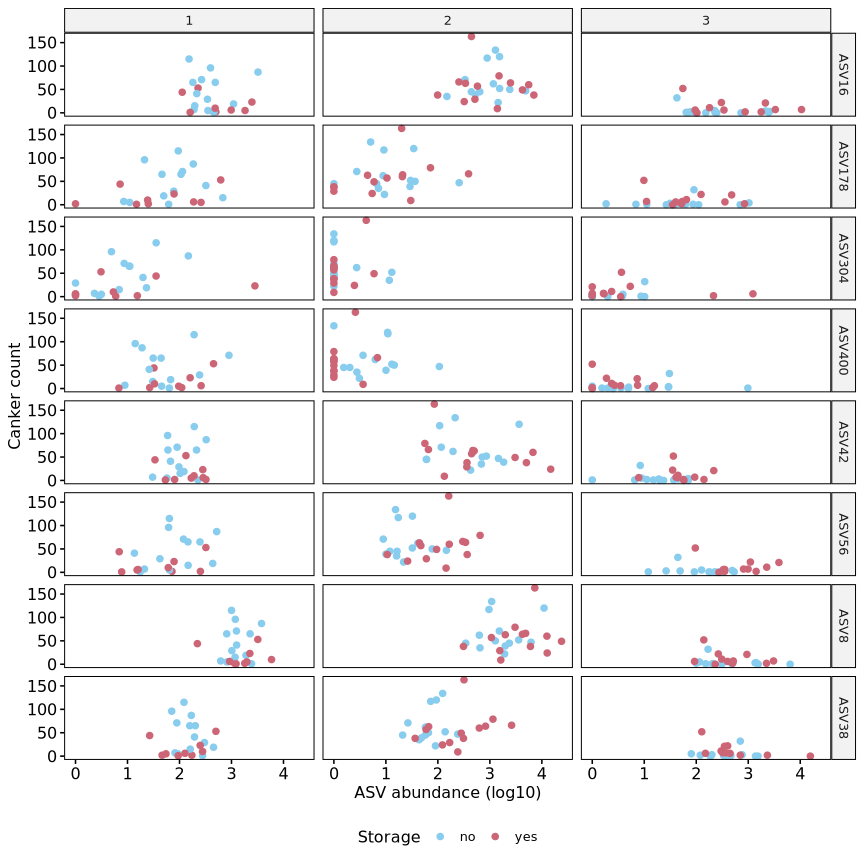
\includegraphics{root_endophytes_files/figure-latex/unnamed-chunk-29-1.pdf}

\hypertarget{permutation-based-anova-on-diversity-index-ranks-1}{%
\subsection{Permutation based anova on diversity index
ranks}\label{permutation-based-anova-on-diversity-index-ranks-1}}

\begin{Shaded}
\begin{Highlighting}[]
\CommentTok{\# get the diversity index data}
\NormalTok{all\_alpha\_ord }\OtherTok{\textless{}{-}} \FunctionTok{plot\_alpha}\NormalTok{(}
  \FunctionTok{counts}\NormalTok{(dds, }\AttributeTok{normalize =}\NormalTok{ F), }\FunctionTok{colData}\NormalTok{(dds), }\AttributeTok{design =} \StringTok{"trial"}\NormalTok{, }\AttributeTok{returnData =}\NormalTok{ T}
\NormalTok{)}

\CommentTok{\# join diversity indices and metadata}
\NormalTok{all\_alpha\_ord }\OtherTok{\textless{}{-}}\NormalTok{ all\_alpha\_ord[}
  \FunctionTok{as.data.table}\NormalTok{(}\FunctionTok{colData}\NormalTok{(dds), }\AttributeTok{keep.rownames =} \StringTok{"Samples"}\NormalTok{), on }\OtherTok{=} \StringTok{"Samples"}
\NormalTok{]}

\NormalTok{formula }\OtherTok{\textless{}{-}}\NormalTok{ DESIGN}
\end{Highlighting}
\end{Shaded}

\hypertarget{chao1-1}{%
\subsubsection{Chao1}\label{chao1-1}}

\begin{Shaded}
\begin{Highlighting}[]
\FunctionTok{setkey}\NormalTok{(all\_alpha\_ord, S.chao1)}
\NormalTok{all\_alpha\_ord[, measure }\SpecialCharTok{:}\ErrorTok{=} \FunctionTok{as.numeric}\NormalTok{(}\FunctionTok{as.factor}\NormalTok{(S.chao1))]}
\FunctionTok{summary}\NormalTok{(}\FunctionTok{aovp}\NormalTok{(}\FunctionTok{update}\NormalTok{(formula, measure }\SpecialCharTok{\textasciitilde{}}\NormalTok{ .), all\_alpha\_ord, }\AttributeTok{seqs =}\NormalTok{ T))}
\end{Highlighting}
\end{Shaded}

\begin{verbatim}
# [1] "Settings:  sequential SS "
\end{verbatim}

\begin{verbatim}
# Component 1 :
#                  Df R Sum Sq R Mean Sq Iter Pr(Prob)    
# trial1            2  20914.4   10457.2 5000   <2e-16 ***
# planting_season1  1    113.5     113.5  100   0.5000    
# cultivar1         6   1194.0     199.0  394   0.6345    
# Residuals        72  23718.6     329.4                  
# ---
# Signif. codes:  0 '***' 0.001 '**' 0.01 '*' 0.05 '.' 0.1 ' ' 1
\end{verbatim}

\hypertarget{shannon-1}{%
\subsubsection{Shannon}\label{shannon-1}}

\begin{Shaded}
\begin{Highlighting}[]
\FunctionTok{setkey}\NormalTok{(all\_alpha\_ord, shannon)}
\NormalTok{all\_alpha\_ord[, measure }\SpecialCharTok{:}\ErrorTok{=} \FunctionTok{as.numeric}\NormalTok{(}\FunctionTok{as.factor}\NormalTok{(shannon))]}
\FunctionTok{summary}\NormalTok{(}\FunctionTok{aovp}\NormalTok{(}\FunctionTok{update}\NormalTok{(formula, measure }\SpecialCharTok{\textasciitilde{}}\NormalTok{ .), all\_alpha\_ord, }\AttributeTok{seqs =}\NormalTok{ T))}
\end{Highlighting}
\end{Shaded}

\begin{verbatim}
# [1] "Settings:  sequential SS "
\end{verbatim}

\begin{verbatim}
# Component 1 :
#                  Df R Sum Sq R Mean Sq Iter Pr(Prob)    
# trial1            2  23583.2   11791.6 5000   <2e-16 ***
# planting_season1  1     89.3      89.3   51   0.9804    
# cultivar1         6    974.0     162.3  312   0.7308    
# Residuals        72  21294.0     295.8                  
# ---
# Signif. codes:  0 '***' 0.001 '**' 0.01 '*' 0.05 '.' 0.1 ' ' 1
\end{verbatim}

\hypertarget{simpson-1}{%
\subsubsection{Simpson}\label{simpson-1}}

\begin{Shaded}
\begin{Highlighting}[]
\FunctionTok{setkey}\NormalTok{(all\_alpha\_ord, simpson)}
\NormalTok{all\_alpha\_ord[, measure }\SpecialCharTok{:}\ErrorTok{=} \FunctionTok{as.numeric}\NormalTok{(}\FunctionTok{as.factor}\NormalTok{(simpson))]}
\FunctionTok{summary}\NormalTok{(}\FunctionTok{aovp}\NormalTok{(}\FunctionTok{update}\NormalTok{(formula, measure }\SpecialCharTok{\textasciitilde{}}\NormalTok{ .), all\_alpha\_ord, }\AttributeTok{seqs =}\NormalTok{ T))}
\end{Highlighting}
\end{Shaded}

\begin{verbatim}
# [1] "Settings:  sequential SS "
\end{verbatim}

\begin{verbatim}
# Component 1 :
#                  Df R Sum Sq R Mean Sq Iter Pr(Prob)    
# trial1            2  20851.3   10425.7 5000   <2e-16 ***
# planting_season1  1     31.0      31.0   51   0.7255    
# cultivar1         6   1936.5     322.7  586   0.3345    
# Residuals        72  23121.7     321.1                  
# ---
# Signif. codes:  0 '***' 0.001 '**' 0.01 '*' 0.05 '.' 0.1 ' ' 1
\end{verbatim}

\hypertarget{beta-diversity-pcanmds-1}{%
\section{Beta diversity PCA/NMDS}\label{beta-diversity-pcanmds-1}}

\hypertarget{pca-1}{%
\subsection{PCA}\label{pca-1}}

\begin{Shaded}
\begin{Highlighting}[]
\CommentTok{\# perform PC decomposition of DES object}
\NormalTok{mypca }\OtherTok{\textless{}{-}} \FunctionTok{des\_to\_pca}\NormalTok{(dds)}

\CommentTok{\# to get pca plot axis into the same scale create a dataframe of PC scores multiplied by their variance}
\NormalTok{d }\OtherTok{\textless{}{-}} \FunctionTok{t}\NormalTok{(}\FunctionTok{data.frame}\NormalTok{(}\FunctionTok{t}\NormalTok{(mypca}\SpecialCharTok{$}\NormalTok{x) }\SpecialCharTok{*}\NormalTok{ mypca}\SpecialCharTok{$}\NormalTok{percentVar))}

\NormalTok{formula }\OtherTok{=}\NormalTok{ DESIGN}
\end{Highlighting}
\end{Shaded}

\hypertarget{percent-variation-in-first-4-pcs-1}{%
\subsubsection{Percent variation in first 4
PCs}\label{percent-variation-in-first-4-pcs-1}}

\begin{Shaded}
\begin{Highlighting}[]
\NormalTok{pca\_var }\OtherTok{\textless{}{-}} \FunctionTok{data.frame}\NormalTok{(}
  \AttributeTok{row.names =} \FunctionTok{c}\NormalTok{(}\StringTok{"PC1"}\NormalTok{, }\StringTok{"PC2"}\NormalTok{, }\StringTok{"PC3"}\NormalTok{, }\StringTok{"PC4"}\NormalTok{),}
  \AttributeTok{perc\_var =} \FunctionTok{round}\NormalTok{(mypca}\SpecialCharTok{$}\NormalTok{percentVar[}\DecValTok{1}\SpecialCharTok{:}\DecValTok{4}\NormalTok{] }\SpecialCharTok{*} \DecValTok{100}\NormalTok{, }\DecValTok{3}\NormalTok{)}
\NormalTok{)}

\NormalTok{pca\_var}
\end{Highlighting}
\end{Shaded}

\begin{verbatim}
#     perc_var
# PC1   18.589
# PC2   12.716
# PC3    7.053
# PC4    4.031
\end{verbatim}

\hypertarget{anova-of-first-4-pcs-1}{%
\subsubsection{ANOVA of first 4 PCs}\label{anova-of-first-4-pcs-1}}

\begin{Shaded}
\begin{Highlighting}[]
\NormalTok{pca\_summary }\OtherTok{\textless{}{-}} \FunctionTok{apply}\NormalTok{(}
\NormalTok{  mypca}\SpecialCharTok{$}\NormalTok{x[, }\DecValTok{1}\SpecialCharTok{:}\DecValTok{4}\NormalTok{], }\DecValTok{2}\NormalTok{, }
  \ControlFlowTok{function}\NormalTok{(x)\{}
    \FunctionTok{summary}\NormalTok{(}\FunctionTok{aov}\NormalTok{(}\FunctionTok{update}\NormalTok{(formula, x }\SpecialCharTok{\textasciitilde{}}\NormalTok{ .), }\AttributeTok{data =} \FunctionTok{as.data.frame}\NormalTok{(}\FunctionTok{cbind}\NormalTok{(x, }\FunctionTok{colData}\NormalTok{(dds)))))}
\NormalTok{  \}}
\NormalTok{)}

\NormalTok{pca\_summary}
\end{Highlighting}
\end{Shaded}

\begin{verbatim}
# $PC1
#                 Df Sum Sq Mean Sq F value Pr(>F)    
# trial            2 190646   95323 198.165 <2e-16 ***
# planting_season  1     25      25   0.051  0.821    
# cultivar         6   4227     704   1.465  0.203    
# Residuals       72  34634     481                   
# ---
# Signif. codes:  0 '***' 0.001 '**' 0.01 '*' 0.05 '.' 0.1 ' ' 1
# 
# $PC2
#                 Df Sum Sq Mean Sq F value Pr(>F)    
# trial            2 137668   68834 279.576 <2e-16 ***
# planting_season  1    142     142   0.578  0.450    
# cultivar         6   1474     246   0.998  0.434    
# Residuals       72  17727     246                   
# ---
# Signif. codes:  0 '***' 0.001 '**' 0.01 '*' 0.05 '.' 0.1 ' ' 1
# 
# $PC3
#                 Df Sum Sq Mean Sq F value Pr(>F)  
# trial            2   2673  1336.5   1.361  0.263  
# planting_season  1     30    30.2   0.031  0.861  
# cultivar         6  13665  2277.6   2.319  0.042 *
# Residuals       72  70716   982.2                 
# ---
# Signif. codes:  0 '***' 0.001 '**' 0.01 '*' 0.05 '.' 0.1 ' ' 1
# 
# $PC4
#                 Df Sum Sq Mean Sq F value Pr(>F)  
# trial            2   5281  2640.3   4.672 0.0124 *
# planting_season  1    635   634.6   1.123 0.2928  
# cultivar         6   3161   526.9   0.932 0.4773  
# Residuals       72  40692   565.2                 
# ---
# Signif. codes:  0 '***' 0.001 '**' 0.01 '*' 0.05 '.' 0.1 ' ' 1
\end{verbatim}

\hypertarget{percent-variation-in-first-4-pcs-for-each-factor-1}{%
\subsubsection{Percent variation in first 4 PCs for each
factor}\label{percent-variation-in-first-4-pcs-for-each-factor-1}}

\begin{Shaded}
\begin{Highlighting}[]
\NormalTok{pcas }\OtherTok{\textless{}{-}} \FunctionTok{list}\NormalTok{(}
  \AttributeTok{PC1 =} \FunctionTok{data.frame}\NormalTok{(}\FunctionTok{unclass}\NormalTok{(pca\_summary}\SpecialCharTok{$}\NormalTok{PC1)),}
  \AttributeTok{PC2 =} \FunctionTok{data.frame}\NormalTok{(}\FunctionTok{unclass}\NormalTok{(pca\_summary}\SpecialCharTok{$}\NormalTok{PC2)),}
  \AttributeTok{PC3 =} \FunctionTok{data.frame}\NormalTok{(}\FunctionTok{unclass}\NormalTok{(pca\_summary}\SpecialCharTok{$}\NormalTok{PC3)),}
  \AttributeTok{PC4 =} \FunctionTok{data.frame}\NormalTok{(}\FunctionTok{unclass}\NormalTok{(pca\_summary}\SpecialCharTok{$}\NormalTok{PC4))}
\NormalTok{)}

\NormalTok{pca\_factors }\OtherTok{\textless{}{-}} \FunctionTok{data.table}\NormalTok{(}
  \AttributeTok{PCs =} \FunctionTok{names}\NormalTok{(pcas),}
  \AttributeTok{total\_var =}\NormalTok{ pca\_var}\SpecialCharTok{$}\NormalTok{perc\_var,}
  \AttributeTok{site\_var =} \FunctionTok{sapply}\NormalTok{(pcas, }\ControlFlowTok{function}\NormalTok{(x) (x[}\StringTok{\textquotesingle{}trial\textquotesingle{}}\NormalTok{, }\StringTok{\textquotesingle{}Sum.Sq\textquotesingle{}}\NormalTok{] }\SpecialCharTok{/} \FunctionTok{sum}\NormalTok{(x[}\StringTok{\textquotesingle{}Sum.Sq\textquotesingle{}}\NormalTok{])) }\SpecialCharTok{*} \DecValTok{100}\NormalTok{),}
  \AttributeTok{site\_p =} \FunctionTok{sapply}\NormalTok{(pcas, }\ControlFlowTok{function}\NormalTok{(x) x[}\StringTok{\textquotesingle{}trial\textquotesingle{}}\NormalTok{, }\StringTok{\textquotesingle{}Pr..F.\textquotesingle{}}\NormalTok{]),}
  \AttributeTok{cultivar\_var =} \FunctionTok{sapply}\NormalTok{(pcas, }\ControlFlowTok{function}\NormalTok{(x) (x[}\StringTok{\textquotesingle{}cultivar\textquotesingle{}}\NormalTok{, }\StringTok{\textquotesingle{}Sum.Sq\textquotesingle{}}\NormalTok{] }\SpecialCharTok{/} \FunctionTok{sum}\NormalTok{(x[}\StringTok{\textquotesingle{}Sum.Sq\textquotesingle{}}\NormalTok{])) }\SpecialCharTok{*} \DecValTok{100}\NormalTok{),}
  \AttributeTok{cultivar\_p =} \FunctionTok{sapply}\NormalTok{(pcas, }\ControlFlowTok{function}\NormalTok{(x) x[}\StringTok{\textquotesingle{}cultivar\textquotesingle{}}\NormalTok{, }\StringTok{\textquotesingle{}Pr..F.\textquotesingle{}}\NormalTok{]),}
  \AttributeTok{season\_var =} \FunctionTok{sapply}\NormalTok{(pcas, }\ControlFlowTok{function}\NormalTok{(x) (x[}\StringTok{\textquotesingle{}planting\_season\textquotesingle{}}\NormalTok{, }\StringTok{\textquotesingle{}Sum.Sq\textquotesingle{}}\NormalTok{] }\SpecialCharTok{/} \FunctionTok{sum}\NormalTok{(x[}\StringTok{\textquotesingle{}Sum.Sq\textquotesingle{}}\NormalTok{])) }\SpecialCharTok{*} \DecValTok{100}\NormalTok{),}
  \AttributeTok{season\_p =} \FunctionTok{sapply}\NormalTok{(pcas, }\ControlFlowTok{function}\NormalTok{(x) x[}\StringTok{\textquotesingle{}planting\_season\textquotesingle{}}\NormalTok{, }\StringTok{\textquotesingle{}Pr..F.\textquotesingle{}}\NormalTok{]),}
  \AttributeTok{residuals\_var =} \FunctionTok{sapply}\NormalTok{(pcas, }\ControlFlowTok{function}\NormalTok{(x) (x[}\StringTok{\textquotesingle{}Residuals\textquotesingle{}}\NormalTok{, }\StringTok{\textquotesingle{}Sum.Sq\textquotesingle{}}\NormalTok{] }\SpecialCharTok{/} \FunctionTok{sum}\NormalTok{(x[}\StringTok{\textquotesingle{}Sum.Sq\textquotesingle{}}\NormalTok{])) }\SpecialCharTok{*} \DecValTok{100}\NormalTok{)}
\NormalTok{)}

\NormalTok{pca\_factors}
\end{Highlighting}
\end{Shaded}

\begin{verbatim}
#    PCs total_var site_var       site_p cultivar_var cultivar_p season_var  season_p residuals_var
# 1: PC1    18.589 83.05869 5.297482e-30    1.8415494 0.20261215 0.01078910 0.8211467      15.08897
# 2: PC2    12.716 87.68034 1.145889e-34    0.9387968 0.43355246 0.09058350 0.4497102      11.29028
# 3: PC3     7.053  3.06951 2.629694e-01   15.6922358 0.04200419 0.03467387 0.8613050      81.20358
# 4: PC4     4.031 10.61034 1.236963e-02    6.3519788 0.47732602 1.27508580 0.2928500      81.76259
\end{verbatim}

\hypertarget{pca-plot-1}{%
\subsubsection{PCA plot}\label{pca-plot-1}}

\begin{Shaded}
\begin{Highlighting}[]
\NormalTok{bac\_pca\_plot }\OtherTok{\textless{}{-}} \FunctionTok{plotOrd}\NormalTok{(}
\NormalTok{  d,}
  \FunctionTok{colData}\NormalTok{(dds),}
  \AttributeTok{design =} \StringTok{"cultivar"}\NormalTok{,}
  \AttributeTok{shape =} \StringTok{"trial"}\NormalTok{,}
  \AttributeTok{axes =} \FunctionTok{c}\NormalTok{(}\DecValTok{1}\NormalTok{, }\DecValTok{2}\NormalTok{),}
  \AttributeTok{facet =} \StringTok{"planting\_season"}\NormalTok{, }
  \AttributeTok{cbPalette =}\NormalTok{ T,}
  \AttributeTok{alpha =} \FloatTok{0.75}\NormalTok{,}
\NormalTok{) }\CommentTok{\#+ facet\_wrap(\textasciitilde{}facet) }

\FunctionTok{ggsave}\NormalTok{(}\AttributeTok{filename =} \StringTok{"bac\_pca\_plot.png"}\NormalTok{, }\AttributeTok{plot =}\NormalTok{ bac\_pca\_plot, }\AttributeTok{path =} \StringTok{"figures/"}\NormalTok{)}

\NormalTok{bac\_pca\_plot}
\end{Highlighting}
\end{Shaded}

\includegraphics{root_endophytes_files/figure-latex/unnamed-chunk-38-1.pdf}

\hypertarget{pca-sum-of-squares-var-1}{%
\subsubsection{PCA sum of squares (\%
var)}\label{pca-sum-of-squares-var-1}}

\begin{Shaded}
\begin{Highlighting}[]
\NormalTok{sum\_squares }\OtherTok{\textless{}{-}} \FunctionTok{apply}\NormalTok{(mypca}\SpecialCharTok{$}\NormalTok{x, }\DecValTok{2}\NormalTok{ ,}\ControlFlowTok{function}\NormalTok{(x) }
  \FunctionTok{summary}\NormalTok{(}\FunctionTok{aov}\NormalTok{(}\FunctionTok{update}\NormalTok{(formula, x }\SpecialCharTok{\textasciitilde{}}\NormalTok{ .), }\AttributeTok{data =} \FunctionTok{cbind}\NormalTok{(x, }\FunctionTok{colData}\NormalTok{(dds))))[[}\DecValTok{1}\NormalTok{]][}\DecValTok{2}\NormalTok{]}
\NormalTok{)}
\NormalTok{sum\_squares }\OtherTok{\textless{}{-}} \FunctionTok{do.call}\NormalTok{(cbind, sum\_squares)}
\NormalTok{x }\OtherTok{\textless{}{-}} \FunctionTok{t}\NormalTok{(}\FunctionTok{apply}\NormalTok{(sum\_squares, }\DecValTok{2}\NormalTok{, prop.table))}
\NormalTok{perVar }\OtherTok{\textless{}{-}}\NormalTok{ x }\SpecialCharTok{*}\NormalTok{ mypca}\SpecialCharTok{$}\NormalTok{percentVar}
\CommentTok{\#colSums(perVar)}
\FunctionTok{round}\NormalTok{(}\FunctionTok{colSums}\NormalTok{(perVar) }\SpecialCharTok{/} \FunctionTok{sum}\NormalTok{(}\FunctionTok{colSums}\NormalTok{(perVar)) }\SpecialCharTok{*} \DecValTok{100}\NormalTok{, }\DecValTok{3}\NormalTok{)}
\end{Highlighting}
\end{Shaded}

\begin{verbatim}
# trial           planting_season cultivar        Residuals       
#          27.377           1.163           6.201          65.260
\end{verbatim}

\hypertarget{adonis-1}{%
\subsection{ADONIS}\label{adonis-1}}

\begin{Shaded}
\begin{Highlighting}[]
\NormalTok{vg }\OtherTok{\textless{}{-}} \FunctionTok{vegdist}\NormalTok{(}\FunctionTok{t}\NormalTok{(}\FunctionTok{counts}\NormalTok{(dds, }\AttributeTok{normalize =}\NormalTok{ DNORM)), }\AttributeTok{method =} \StringTok{"bray"}\NormalTok{)}
\FunctionTok{set.seed}\NormalTok{(}\FunctionTok{sum}\NormalTok{(}\FunctionTok{utf8ToInt}\NormalTok{(}\StringTok{"Hamish McLean"}\NormalTok{)))}
\FunctionTok{adonis2}\NormalTok{(}\FunctionTok{update}\NormalTok{(formula, vg }\SpecialCharTok{\textasciitilde{}}\NormalTok{ .), }\FunctionTok{colData}\NormalTok{(dds), }\AttributeTok{permutations =} \DecValTok{1000}\NormalTok{)}
\end{Highlighting}
\end{Shaded}

\begin{verbatim}
# Permutation test for adonis under reduced model
# Terms added sequentially (first to last)
# Permutation: free
# Number of permutations: 1000
# 
# adonis2(formula = update(formula, vg ~ .), data = colData(dds), permutations = 1000)
#                 Df SumOfSqs      R2       F   Pr(>F)    
# trial            2   3.8107 0.32376 19.1727 0.000999 ***
# planting_season  1   0.2026 0.01721  2.0386 0.028971 *  
# cultivar         6   0.6015 0.05111  1.0088 0.429570    
# Residual        72   7.1552 0.60792                     
# Total           81  11.7700 1.00000                     
# ---
# Signif. codes:  0 '***' 0.001 '**' 0.01 '*' 0.05 '.' 0.1 ' ' 1
\end{verbatim}

\hypertarget{nmds-ordination-1}{%
\subsection{NMDS ordination}\label{nmds-ordination-1}}

\begin{Shaded}
\begin{Highlighting}[]
\FunctionTok{set.seed}\NormalTok{(}\FunctionTok{sum}\NormalTok{(}\FunctionTok{utf8ToInt}\NormalTok{(}\StringTok{"Hamish McLean"}\NormalTok{)))}
\NormalTok{ord }\OtherTok{\textless{}{-}} \FunctionTok{metaMDS}\NormalTok{(vg,}\AttributeTok{trace=}\DecValTok{0}\NormalTok{) }
\CommentTok{\#sratmax=20000,maxit=20000,try = 177, trymax = 177}

\NormalTok{nmds }\OtherTok{\textless{}{-}} \FunctionTok{scores}\NormalTok{(ord)}

\NormalTok{bac\_nmds\_plot }\OtherTok{\textless{}{-}} \FunctionTok{plotOrd}\NormalTok{(}
\NormalTok{  nmds, }\FunctionTok{colData}\NormalTok{(dds), }\AttributeTok{design =}\NormalTok{ Factor2, }
  \AttributeTok{shape =}\NormalTok{ Factor1, }\AttributeTok{alpha =} \FloatTok{0.75}\NormalTok{, }\AttributeTok{cbPalette =}\NormalTok{ T}
\NormalTok{) }\SpecialCharTok{+} \FunctionTok{theme}\NormalTok{(}\AttributeTok{text =} \FunctionTok{element\_text}\NormalTok{(}\AttributeTok{size =} \DecValTok{14}\NormalTok{))}

\FunctionTok{ggsave}\NormalTok{(}\AttributeTok{filename =} \StringTok{"fun\_nmds\_plot.png"}\NormalTok{, }\AttributeTok{plot =}\NormalTok{ bac\_nmds\_plot, }\AttributeTok{path =} \StringTok{"figures/"}\NormalTok{)}

\NormalTok{bac\_nmds\_plot}
\end{Highlighting}
\end{Shaded}

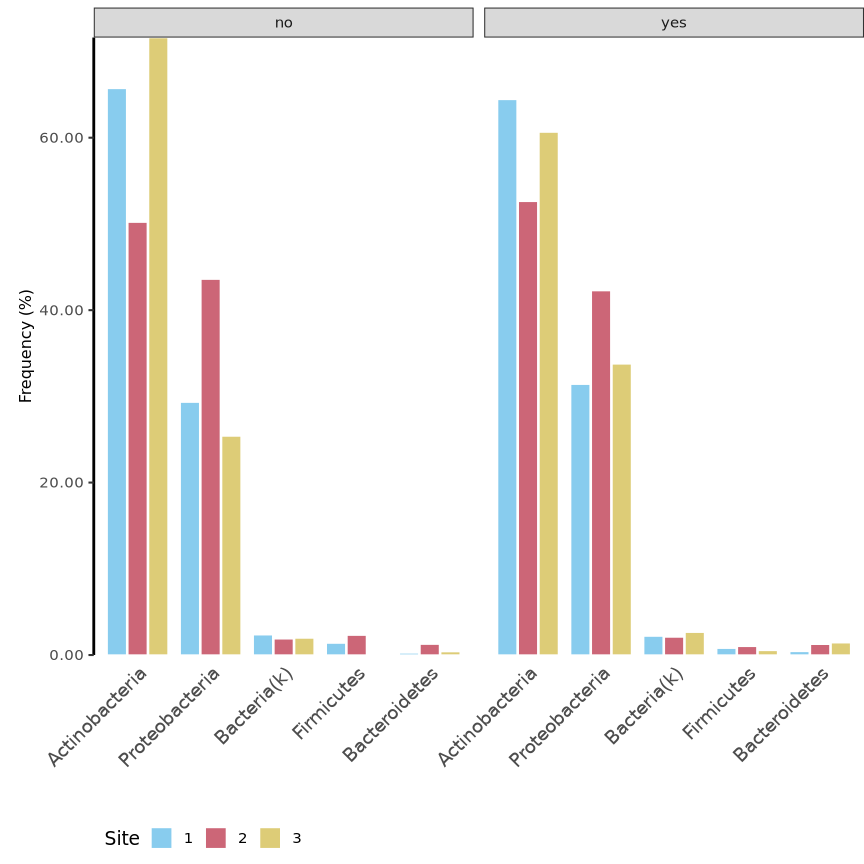
\includegraphics{root_endophytes_files/figure-latex/unnamed-chunk-41-1.pdf}

\hypertarget{nmds-with-phylum-or-class-arrows-1}{%
\subsubsection{NMDS with phylum or class
arrows}\label{nmds-with-phylum-or-class-arrows-1}}

\begin{Shaded}
\begin{Highlighting}[]
\NormalTok{otus }\OtherTok{\textless{}{-}} \FunctionTok{scores}\NormalTok{(ord,}\StringTok{"species"}\NormalTok{) }

\NormalTok{taxmerge }\OtherTok{\textless{}{-}}\FunctionTok{data.table}\NormalTok{(}\FunctionTok{inner\_join}\NormalTok{(}\FunctionTok{data.table}\NormalTok{(}\AttributeTok{OTU=}\FunctionTok{rownames}\NormalTok{(otus),}\FunctionTok{as.data.frame}\NormalTok{(otus)),}\FunctionTok{data.table}\NormalTok{(}\AttributeTok{OTU=}\FunctionTok{rownames}\NormalTok{(taxData),taxData))) }
\end{Highlighting}
\end{Shaded}

\begin{verbatim}
# Error in `inner_join()`:
# ! `by` must be supplied when `x` and `y` have no common variables.
# i Use `cross_join()` to perform a cross-join.
\end{verbatim}

\begin{Shaded}
\begin{Highlighting}[]
\NormalTok{taxmerge}\SpecialCharTok{$}\NormalTok{phy }\OtherTok{\textless{}{-}} \FunctionTok{taxaConfVec}\NormalTok{(taxmerge[,}\FunctionTok{c}\NormalTok{(}\SpecialCharTok{{-}}\DecValTok{1}\SpecialCharTok{:{-}}\DecValTok{3}\NormalTok{,}\SpecialCharTok{{-}}\DecValTok{8}\NormalTok{)],}\AttributeTok{conf=}\FloatTok{0.9}\NormalTok{,}\AttributeTok{level=}\FunctionTok{which}\NormalTok{(}\FunctionTok{colnames}\NormalTok{(taxmerge[,}\FunctionTok{c}\NormalTok{(}\SpecialCharTok{{-}}\DecValTok{1}\SpecialCharTok{:{-}}\DecValTok{3}\NormalTok{,}\SpecialCharTok{{-}}\DecValTok{8}\NormalTok{)])}\SpecialCharTok{==}\StringTok{"phylum"}\NormalTok{))}
\end{Highlighting}
\end{Shaded}

\begin{verbatim}
# Error in apply(obj, 1, function(x) {: object 'taxmerge' not found
\end{verbatim}

\begin{Shaded}
\begin{Highlighting}[]
\NormalTok{taxmerge}\SpecialCharTok{$}\NormalTok{cls }\OtherTok{\textless{}{-}} \FunctionTok{taxaConfVec}\NormalTok{(taxmerge[,}\FunctionTok{c}\NormalTok{(}\SpecialCharTok{{-}}\DecValTok{1}\SpecialCharTok{:{-}}\DecValTok{3}\NormalTok{,}\SpecialCharTok{{-}}\DecValTok{8}\NormalTok{)],}\AttributeTok{conf=}\FloatTok{0.9}\NormalTok{,}\AttributeTok{level=}\FunctionTok{which}\NormalTok{(}\FunctionTok{colnames}\NormalTok{(taxmerge[,}\FunctionTok{c}\NormalTok{(}\SpecialCharTok{{-}}\DecValTok{1}\SpecialCharTok{:{-}}\DecValTok{3}\NormalTok{,}\SpecialCharTok{{-}}\DecValTok{8}\NormalTok{)])}\SpecialCharTok{==}\StringTok{"class"}\NormalTok{)) }
\end{Highlighting}
\end{Shaded}

\begin{verbatim}
# Error in apply(obj, 1, function(x) {: object 'taxmerge' not found
\end{verbatim}

\begin{Shaded}
\begin{Highlighting}[]
\NormalTok{phy }\OtherTok{\textless{}{-}}\NormalTok{ taxmerge[,}\FunctionTok{lapply}\NormalTok{(.SD,mean),by}\OtherTok{=}\NormalTok{phy,.SDcols}\OtherTok{=}\FunctionTok{c}\NormalTok{(}\StringTok{"NMDS1"}\NormalTok{,}\StringTok{"NMDS2"}\NormalTok{)]}
\end{Highlighting}
\end{Shaded}

\begin{verbatim}
# Error in eval(expr, envir, enclos): object 'taxmerge' not found
\end{verbatim}

\begin{Shaded}
\begin{Highlighting}[]
\NormalTok{cls }\OtherTok{\textless{}{-}}\NormalTok{ taxmerge[,}\FunctionTok{lapply}\NormalTok{(.SD,mean),by}\OtherTok{=}\NormalTok{cls,.SDcols}\OtherTok{=}\FunctionTok{c}\NormalTok{(}\StringTok{"NMDS1"}\NormalTok{,}\StringTok{"NMDS2"}\NormalTok{)]}
\end{Highlighting}
\end{Shaded}

\begin{verbatim}
# Error in eval(expr, envir, enclos): object 'taxmerge' not found
\end{verbatim}

\begin{Shaded}
\begin{Highlighting}[]
\NormalTok{bac\_nmds\_plot }\SpecialCharTok{+} \FunctionTok{geom\_segment}\NormalTok{(}\AttributeTok{inherit.aes =}\NormalTok{ F,}\AttributeTok{data=}\NormalTok{phy,}\FunctionTok{aes}\NormalTok{(}\AttributeTok{xend=}\NormalTok{NMDS1,}\AttributeTok{yend=}\NormalTok{NMDS2,}\AttributeTok{x=}\DecValTok{0}\NormalTok{,}\AttributeTok{y=}\DecValTok{0}\NormalTok{),}\AttributeTok{size=}\FloatTok{1.5}\NormalTok{,}\AttributeTok{arrow=}\FunctionTok{arrow}\NormalTok{()) }\SpecialCharTok{+} 
  \FunctionTok{geom\_text}\NormalTok{(}\AttributeTok{inherit.aes =}\NormalTok{ F,}\AttributeTok{data=}\NormalTok{phy,}\FunctionTok{aes}\NormalTok{(}\AttributeTok{x=}\NormalTok{NMDS1,}\AttributeTok{y=}\NormalTok{(NMDS2}\SpecialCharTok{+}\FunctionTok{sign}\NormalTok{(NMDS2)}\SpecialCharTok{*}\FloatTok{0.05}\NormalTok{),}\AttributeTok{label=}\NormalTok{phy))}
\end{Highlighting}
\end{Shaded}

\begin{verbatim}
# Error in fortify(data): object 'phy' not found
\end{verbatim}

\begin{Shaded}
\begin{Highlighting}[]
\FunctionTok{ggsave}\NormalTok{(}\AttributeTok{filename =} \StringTok{"fun\_nmds\_phy.png"}\NormalTok{, }\AttributeTok{plot =}\NormalTok{ bac\_nmds\_plot, }\AttributeTok{path =} \StringTok{"figures/"}\NormalTok{)}
\end{Highlighting}
\end{Shaded}

\hypertarget{differential-analysis}{%
\section{differential analysis}\label{differential-analysis}}

\hypertarget{deseq-design}{%
\subsection{DESeq design}\label{deseq-design}}

\begin{Shaded}
\begin{Highlighting}[]
\CommentTok{\# p value for FDR cutoff}
\NormalTok{alpha }\OtherTok{\textless{}{-}} \FloatTok{0.1}

\CommentTok{\# add design to dds object}
\FunctionTok{design}\NormalTok{(dds) }\OtherTok{\textless{}{-}}\NormalTok{ formula}
\end{Highlighting}
\end{Shaded}

\begin{verbatim}
# Error in validObject(object): invalid class "DESeqDataSet" object: all variables in design formula must be columns in colData
\end{verbatim}

\begin{Shaded}
\begin{Highlighting}[]
\CommentTok{\# run model}
\NormalTok{dds }\OtherTok{\textless{}{-}} \FunctionTok{DESeq}\NormalTok{(dds,}\AttributeTok{parallel=}\NormalTok{F)}

\CommentTok{\# build results table}
\NormalTok{res }\OtherTok{\textless{}{-}} \FunctionTok{results}\NormalTok{(dds,}\AttributeTok{alpha=}\NormalTok{alpha,}\AttributeTok{contrast=}\FunctionTok{c}\NormalTok{(}\StringTok{"Status"}\NormalTok{,}\StringTok{"Diseased"}\NormalTok{,}\StringTok{"Healthy"}\NormalTok{))}
\end{Highlighting}
\end{Shaded}

\begin{verbatim}
# Error in cleanContrast(object, contrast, expanded = isExpanded, listValues = listValues, : Status should be the name of a factor in the colData of the DESeqDataSet
\end{verbatim}

\hypertarget{result-summary}{%
\subsection{Result summary}\label{result-summary}}

Rank is lowest taxonomic rank with \textgreater=0.65 confidence

\hypertarget{all-samples}{%
\subsubsection{All samples}\label{all-samples}}

\begin{Shaded}
\begin{Highlighting}[]
\FunctionTok{summary}\NormalTok{(res)}
\end{Highlighting}
\end{Shaded}

\begin{verbatim}
# 
# out of 5882 with nonzero total read count
# adjusted p-value < 0.1
# LFC > 0 (up)       : 3300, 56%
# LFC < 0 (down)     : 574, 9.8%
# outliers [1]       : 0, 0%
# low counts [2]     : 1, 0.017%
# (mean count < 0)
# [1] see 'cooksCutoff' argument of ?results
# [2] see 'independentFiltering' argument of ?results
\end{verbatim}

\begin{Shaded}
\begin{Highlighting}[]
\CommentTok{\# merge DESeq results with taxonomy}
\NormalTok{res.merge }\OtherTok{\textless{}{-}} \FunctionTok{as.data.table}\NormalTok{(res,}\AttributeTok{keep.rownames=}\StringTok{"OTU"}\NormalTok{)[}
  \FunctionTok{as.data.table}\NormalTok{(taxData,}\AttributeTok{keep.rownames=}\StringTok{"OTU"}\NormalTok{),on}\OtherTok{=}\StringTok{"OTU"}\NormalTok{]}

\CommentTok{\# print sig. results}
\NormalTok{res.merge[padj}\SpecialCharTok{\textless{}=}\NormalTok{alpha,.(OTU,rank,}
                        \AttributeTok{baseMean=}\FunctionTok{round}\NormalTok{(baseMean,}\DecValTok{2}\NormalTok{),}
                        \AttributeTok{FC=}\FunctionTok{round}\NormalTok{(log2FoldChange,}\DecValTok{2}\NormalTok{),}
                        \AttributeTok{padj=}\FunctionTok{round}\NormalTok{(padj,}\DecValTok{4}\NormalTok{))][}\FunctionTok{order}\NormalTok{(FC,}\AttributeTok{decreasing =}\NormalTok{ T),]}
\end{Highlighting}
\end{Shaded}

\begin{verbatim}
#           OTU                   rank baseMean    FC   padj
#    1:    OTU1        Streptomyces(g)  1700.00 10.73 0.0000
#    2:    OTU2      Kineosporiales(o)  1516.67 10.57 0.0000
#    3:    OTU3     Kineosporiaceae(f)  1387.98 10.44 0.0000
#    4:    OTU4        Streptomyces(g)  1216.14 10.25 0.0000
#    5:    OTU5        Streptomyces(g)  1182.67 10.21 0.0000
#   ---                                                     
# 3870: OTU4752        Myxococcales(o)     0.06 -3.98 0.0006
# 3871: OTU3370 Gammaproteobacteria(c)     0.05 -4.21 0.0102
# 3872: OTU4301      Rhodocyclaceae(f)     0.05 -4.39 0.0049
# 3873: OTU3985  Betaproteobacteria(c)     0.04 -4.83 0.0098
# 3874: OTU1515        Yersiniaceae(f)     0.02 -5.73 0.0057
\end{verbatim}

\hypertarget{differential-analysis-1}{%
\section{Differential analysis}\label{differential-analysis-1}}

\hypertarget{deseq-design-1}{%
\subsection{DESeq design}\label{deseq-design-1}}

\begin{Shaded}
\begin{Highlighting}[]
\CommentTok{\# P value for FDR cutoff}
\NormalTok{alpha }\OtherTok{\textless{}{-}}\NormalTok{ ALPHA}

\CommentTok{\# Model design}
\NormalTok{formula }\OtherTok{\textless{}{-}} \ErrorTok{\textasciitilde{}}\NormalTok{ mainstem}

\CommentTok{\# Add design to dds object}
\FunctionTok{design}\NormalTok{(dds) }\OtherTok{\textless{}{-}}\NormalTok{ formula}
\end{Highlighting}
\end{Shaded}

\begin{verbatim}
# Error in validObject(object): invalid class "DESeqDataSet" object: all variables in design formula must be columns in colData
\end{verbatim}

\begin{Shaded}
\begin{Highlighting}[]
\CommentTok{\# Run model}
\NormalTok{dds }\OtherTok{\textless{}{-}} \FunctionTok{DESeq}\NormalTok{(dds, }\AttributeTok{parallel=}\NormalTok{F)}

\CommentTok{\# Build results table}
\NormalTok{res }\OtherTok{\textless{}{-}} \FunctionTok{results}\NormalTok{(dds, }\AttributeTok{alpha =}\NormalTok{ alpha)}
\end{Highlighting}
\end{Shaded}

\hypertarget{result-summary-1}{%
\subsubsection{Result summary}\label{result-summary-1}}

Rank is lowest taxonomic rank with \textgreater=0.65 confidence

\hypertarget{all-samples-1}{%
\subsubsection{All samples}\label{all-samples-1}}

\begin{Shaded}
\begin{Highlighting}[]
\FunctionTok{summary}\NormalTok{(res)}
\end{Highlighting}
\end{Shaded}

\begin{verbatim}
# 
# out of 5882 with nonzero total read count
# adjusted p-value < 0.1
# LFC > 0 (up)       : 3300, 56%
# LFC < 0 (down)     : 574, 9.8%
# outliers [1]       : 0, 0%
# low counts [2]     : 1, 0.017%
# (mean count < 0)
# [1] see 'cooksCutoff' argument of ?results
# [2] see 'independentFiltering' argument of ?results
\end{verbatim}

\begin{Shaded}
\begin{Highlighting}[]
\CommentTok{\# merge DESeq results with taxonomy}
\NormalTok{res.merge }\OtherTok{\textless{}{-}} \FunctionTok{as.data.table}\NormalTok{(res,}\AttributeTok{keep.rownames=}\StringTok{"OTU"}\NormalTok{)[}
  \FunctionTok{as.data.table}\NormalTok{(taxData,}\AttributeTok{keep.rownames=}\StringTok{"OTU"}\NormalTok{),on}\OtherTok{=}\StringTok{"OTU"}\NormalTok{]}

\CommentTok{\# print sig. results}
\NormalTok{res.merge[padj}\SpecialCharTok{\textless{}=}\NormalTok{alpha,.(OTU,rank,}
                        \AttributeTok{baseMean=}\FunctionTok{round}\NormalTok{(baseMean,}\DecValTok{2}\NormalTok{),}
                        \AttributeTok{FC=}\FunctionTok{round}\NormalTok{(log2FoldChange,}\DecValTok{2}\NormalTok{),}
                        \AttributeTok{padj=}\FunctionTok{round}\NormalTok{(padj,}\DecValTok{4}\NormalTok{))][}\FunctionTok{order}\NormalTok{(FC,}\AttributeTok{decreasing =}\NormalTok{ T),]}
\end{Highlighting}
\end{Shaded}

\begin{verbatim}
#           OTU                   rank baseMean    FC   padj
#    1:    OTU1        Streptomyces(g)  1700.00 10.73 0.0000
#    2:    OTU2      Kineosporiales(o)  1516.67 10.57 0.0000
#    3:    OTU3     Kineosporiaceae(f)  1387.98 10.44 0.0000
#    4:    OTU4        Streptomyces(g)  1216.14 10.25 0.0000
#    5:    OTU5        Streptomyces(g)  1182.67 10.21 0.0000
#   ---                                                     
# 3870: OTU4752        Myxococcales(o)     0.06 -3.98 0.0006
# 3871: OTU3370 Gammaproteobacteria(c)     0.05 -4.21 0.0102
# 3872: OTU4301      Rhodocyclaceae(f)     0.05 -4.39 0.0049
# 3873: OTU3985  Betaproteobacteria(c)     0.04 -4.83 0.0098
# 3874: OTU1515        Yersiniaceae(f)     0.02 -5.73 0.0057
\end{verbatim}

\end{document}
